\documentclass[a4paper,11pt,twoside]{article}
\usepackage[utf8]{inputenc}
\usepackage[russian]{babel}
\usepackage{dmvn}
\usepackage{wrapfig}
\usepackage[dvips]{graphicx}
\usepackage{multirow}
\usepackage{subfloat}
\usepackage{epigraph}
\usepackage{subfig}
\usepackage{hyperref}
\usepackage{color}

\def\existz{\exists\,!\,}
%% Legacy
\newcommand{\spc}{\colon} 
\newcommand{\ab}{{\bf a}}
\newcommand{\bb}{{\bf b}}
\newcommand{\cb}{{\bf c}}
\newcommand{\eb}{{\bf e}}
\newcommand{\xb}{{\bf x}}
\newcommand\qedsymbol{$\blacktriangleleft$\!}
\newcommand{\adj}{} %It means somtheing I do not understand

%\makeindex

\begin{document}

\author{Boris Agafontsev inspired by Evgeny Golod}
\date{\today}
\title{Algebra}

\dmvntitle{Курс лекций}{по алгебре}{Лектор - Голод Евгений Соломонович}{I курс, 1 семестр, отделение математики}{2006}

\section{Множества и отображения}
\label{sets}
\epigraph{A person who never made a mistake never tried anything new.}{Albert Einstein }

\subsection{Множества}

\begin{df}
	Под \emph{множеством}\index{множество} принято понимать совокупность объектов
	некоторой природы (\emph{множество}~--- неопределяемое понятие). Сами объекты
	называются \emph{элемен\-та\-ми множества}.
\end{df}

\begin{wrapfigure}{r}{3.25cm}
	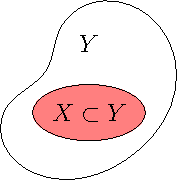
\includegraphics{graph/x-subset-y}
\end{wrapfigure}

Над множествами определено несколько операций:

\begin{description}
	\item[Пересечение]\par\strut\\
		\begin{tabular}{ll}
			\multirow{2}{*}{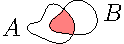
\includegraphics{graph/set-op-intersection}}
				& Обозначается <<$\bigcap$>>. \\
				& $A\bigcap B\eqdef\left\{x\vert x\in A \land x\in B\right\}$
		\end{tabular}
	\item[Объединение]\par\strut\\
		\begin{tabular}{ll}
			\multirow{2}{*}{
\includegraphics{graph/set-op-union}}
				& Обозначается <<$\bigcup$>>. \\
				& $A\bigcup B\eqdef\left\{x\vert x\in A \lor  x\in B\right\}$
		\end{tabular}
	\item[Разность]\par\strut\\
		\begin{tabular}{ll}
			\multirow{2}{*}{
\includegraphics{graph/set-op-difference}}
				& Обозначается <<$\setminus$>>. \\
				& $A\setminus B\eqdef\left\{x\vert x\in A \land x\notin B\right\}$
		\end{tabular}
	\item[Симметрическая разность]\par\strut\\
		\begin{tabular}{ll}			
			\multirow{2}{*}{
\includegraphics{graph/set-op-simmdifference}}
				& Обозначается <<$\Delta$>>. \\
				& $A\Delta B\eqdef(A\setminus B)\cup(B\setminus A)$.
		\end{tabular}
\end{description}

Эти операции обладают следующими свойствами:

\begin{itemize}
	\item Коммутативность пересечения и объединения:
		\begin{align*}
			A\cap B&=B\cap A \\
			A\cup B&=B\cup A
		\end{align*}
	\item Ассоциативность пересечения и объединения:
		\begin{align*}
			(A\cap B)\cap C&=A\cap(B\cap C) \\
			(A\cup B)\cup C&=A\cup(B\cup C)
		\end{align*}
	\item Дистрибутивность пересечения относительно объединения и наоборот.
		\begin{align*}
			(A\cup B)\cap C&=(A\cap C)\cup(B\cap C) \\
			(A\cap B)\cup C&=(A\cup C)\cap(B\cup C)
		\end{align*}
	\item Относительно разности выполняются следующие соотношения:
		\begin{align*}
			M\setminus(A\cap B)&=(M\setminus A)\cup(M\setminus B) \\
			M\setminus(A\cup B)&=(M\setminus A)\cap(M\setminus B)
		\end{align*}
	\item Относительно симметрической разности:
          \begin{align*}
            A\Delta B = (A\cup B)\setminus (A\cap B)
          \end{align*}
    \begin{proof}\par\strut\\
    \begin{enumerate}
      \item Докажем включение $A\Delta B \subset (A\cup B)\setminus (A\cap B)$. 
        Для этого возьмём произвольный элемент $a\in A\Delta B$,
        который по определению содержится в множестве $(A\setminus B)\cup(B\setminus A)$. 
        Возможно две ситуации:
        \begin{enumerate}
          \item $a\in A\setminus B$
          \item $a\in B\setminus A$
        \end{enumerate}
        Пусть имеет место пункт (a).
        Тогда $A\in A,\, a\not\in B\ra a \in A\cup B$ и $a\not\in A\cap B$, откуда явно следует, 
        что $a\in(A\cup B)\setminus (A\cap B)$. При предположении, что имеет место быть 
        пункт (b) рассуждения абсолютно аналогичны.
      
      \item Докажем включение $A\Delta B \supset (A\cup B)\setminus (A\cap B)$. 
        Возьмём произвольный элемент $a\in (A\cup B)\setminus (A\cap B)$, т.е.
        $$
        \left\{
        \begin{array}{l}
          a\in A\cup B\\
          a\not\in A\cap B
        \end{array}
        \right.
        $$
    Возможно две ситуации:
    \begin{enumerate}
      \item $a\in A$
      \item $a\in B$
    \end{enumerate}
    
    Пусть имеет место пункт (a) (для пункта (b) рассуждения проводятся абсолютно аналогично). 
    Так как $a\in A$ и $a\not\in A\cap B$, то $a\not\in B\ra a\in A\setminus B$. 
    Включение доказано.
    \end{enumerate}
    
    Утверждение доказано.
    \end{proof}	
\end{itemize}

\subsection{Отображения}

\begin{df}
Множество $\mathbf D=\mathbf A\times\mathbf B$\index{множество!декартово произведение} называется декартовым (или прямым) произве\-де\-ни\-ем множеств, если оно состоит из всех возможнных пар $(a,b)\colon a\in A,b\in B$ и только из них.
\end{df}

\begin{df}
 Подмножество $\mathbf F$ декартова произведения $\mathbf D =\mathbf A \times\mathbf B$ называется \emph{отобра\-же\-нием}\index{отображение}, если $\forall x\in\mathbf A\spc\exists!(x,y)\in\mathbf F,\spc y\in B$. Тем самым отображение $\mathbf F$ определено на множестве $\mathbf A$. Обозначается следующим образом: $f\colon \Ab\to \Bb$ или $\Ab\stackrel{f}{\to}\Bb$. При этом
пишут, что $y=f(x)$, $x\in \Ab$, $y\in \Bb$, а $y$ называют \emph{образом} $x$\index{образ} (соответственно,
$x$~--- \emph{прообразом} $y$)\index{прообраз}. Множество всех элементов в $\Bb$, у которых есть прообраз в $\Ab$ назывют \emph{полным проообразом}\index{прообраз!полный}. Отображения $f_1$ и $f_2$ из $\Ab$ в $\Bb$ называют равными,
если: $\forall x\in \Ab\spc f_1(x)=f_2(x)$.
 
 %Обозначается $A\xrightarrow{f}B$ или $y = F(x),\spc x\in\mathbf A,y\in\mathbf B$.
\end{df}

Возможно и другое, менее строгое, определение функции. Пусть $\mathbf F$~--- правило, согласно которому каждому $x\in\mathbf A$ ставится в соответствие не более одного элемента $y\in\mathbf B$. В таком случае правило $\mathbf F$ называется функцией. Если у $x$ нет ни одного образа, то говорят, что функция $\mathbf F$ неопределена в точке $x$.\index{функция}

\begin{wrapfigure}[4]{r}{3.25cm}
	\vspace{-.33cm}
	
\includegraphics{graph/mapping-def}
\end{wrapfigure}

Существует классификация отображений, которая выделяет три типа:

\begin{itemize}
	\item\index{отображение!сюрьективное}
		Отображение <<на>>, или \emph{сюръективное отображение}, или
		\emph{сюръекция},~--- это такое отображение, при котором каждый элемент из $Y$
		является образом хотя бы одного элемента из\newline $X$ (см.~рис.~\ref{fig:func:s}).
	\item\index{отображение!инъективное}
		Отображение <<в>>, или \emph{инъективное отображение}, или \emph{инъекция}~--
		это такое отображение, при котором двум разным элементам из $X$ соответствуют
		разные элементы из $Y$: $x_1\ne x_2 \ra f(x_1)\ne f(x_2)$ (см.~рис.~\ref{fig:func:i}).
	\item\index{отображение!биективное}
		Отображение <<между>>, или \emph{биективное отображение}, или \emph{биекция}~---
		это такое отображение, которое является одновременно и сюръекцией, и инъекцией. То
		есть каждому элементу из $X$ соответствует единственный элемент из $Y$ и наоборот.
		Такое отображение также называется взаимнооднозначным (см.~рис.~\ref{fig:func:b}).
\end{itemize}

\begin{figure}[ht]
	\subfloat[Сюръекция]{\label{fig:func:s}
\includegraphics{graph/mapping-3}}
	\hfill
	\subfloat[Биекция]  {\label{fig:func:b}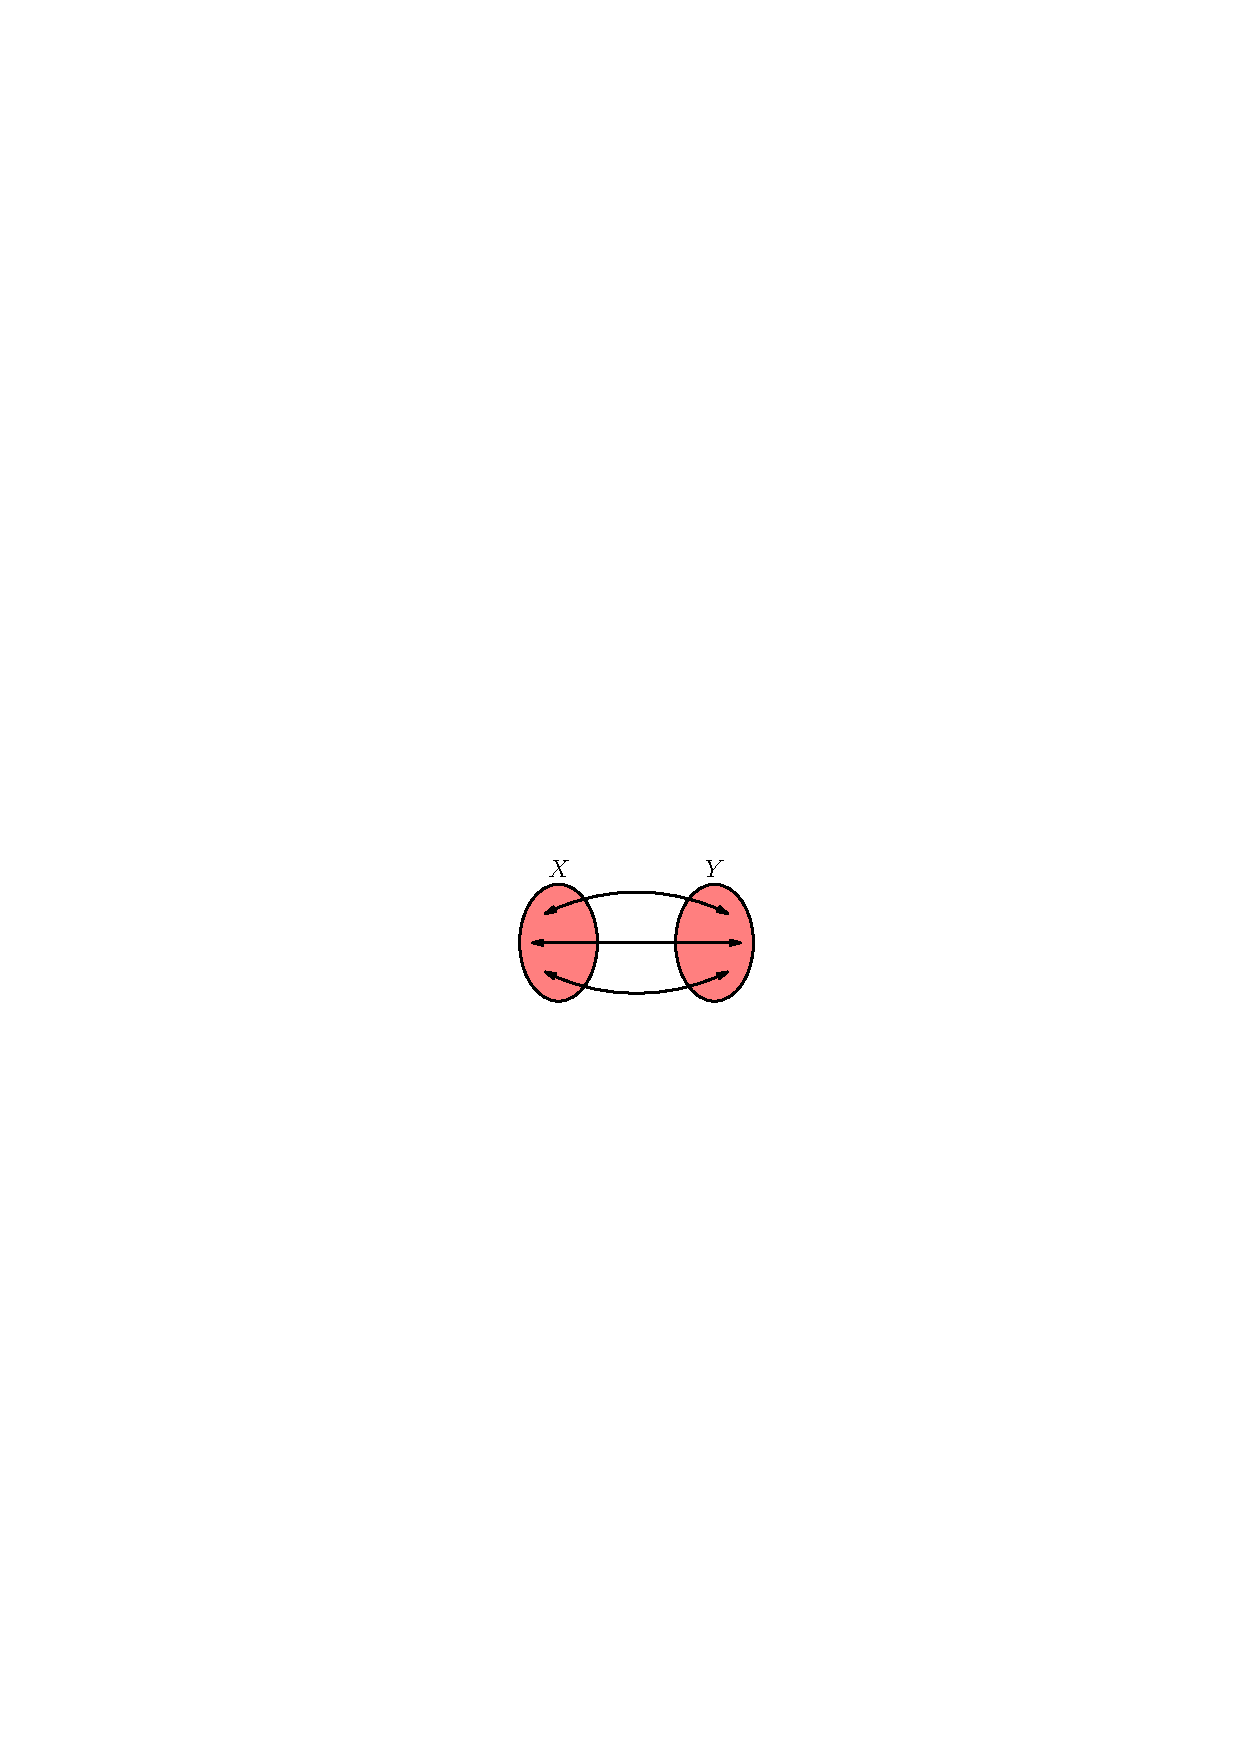
\includegraphics{graph/mapping-2}}
	\hfill
	\subfloat[Инъекция] {\label{fig:func:i}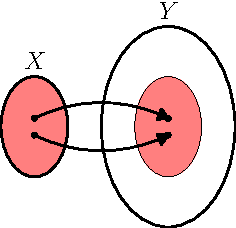
\includegraphics{graph/mapping-1}}
	\caption{Классификация отображений}
\end{figure}

\paragraph{Обратное отображение}

\begin{wrapfigure}[8]{r}{3.25cm}
	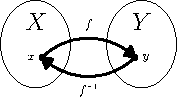
\includegraphics{graph/mapping-rev}
\end{wrapfigure}

Если задано биективное отображение $f\colon X\to Y$, то имеет смысл говорить об
\emph{обратном отображении}\index{отображение!обратное}:
$$\forall y\in Y\existz x\in X\colon y=f(x)$$
$$\exists g\colon Y\to X=f^{-1}\colon f^{-1}(y)=x$$

Очевидно, что $\left(f^{-1}\right)^{-1}\equiv f$.

\paragraph{Композиция отображений}\index{композиция!отображений}

\begin{df}
	Пусть заданы отображения $f\colon X\to Y$ и $g\colon Y\to Z$. Тогда композицией
	отображений $f$ и $g$ называют отображение $(g\circ f)$, которое действует по правилу:

	$$(g\circ f)(x)\eqdef g(f(x))$$

	\begin{center}
		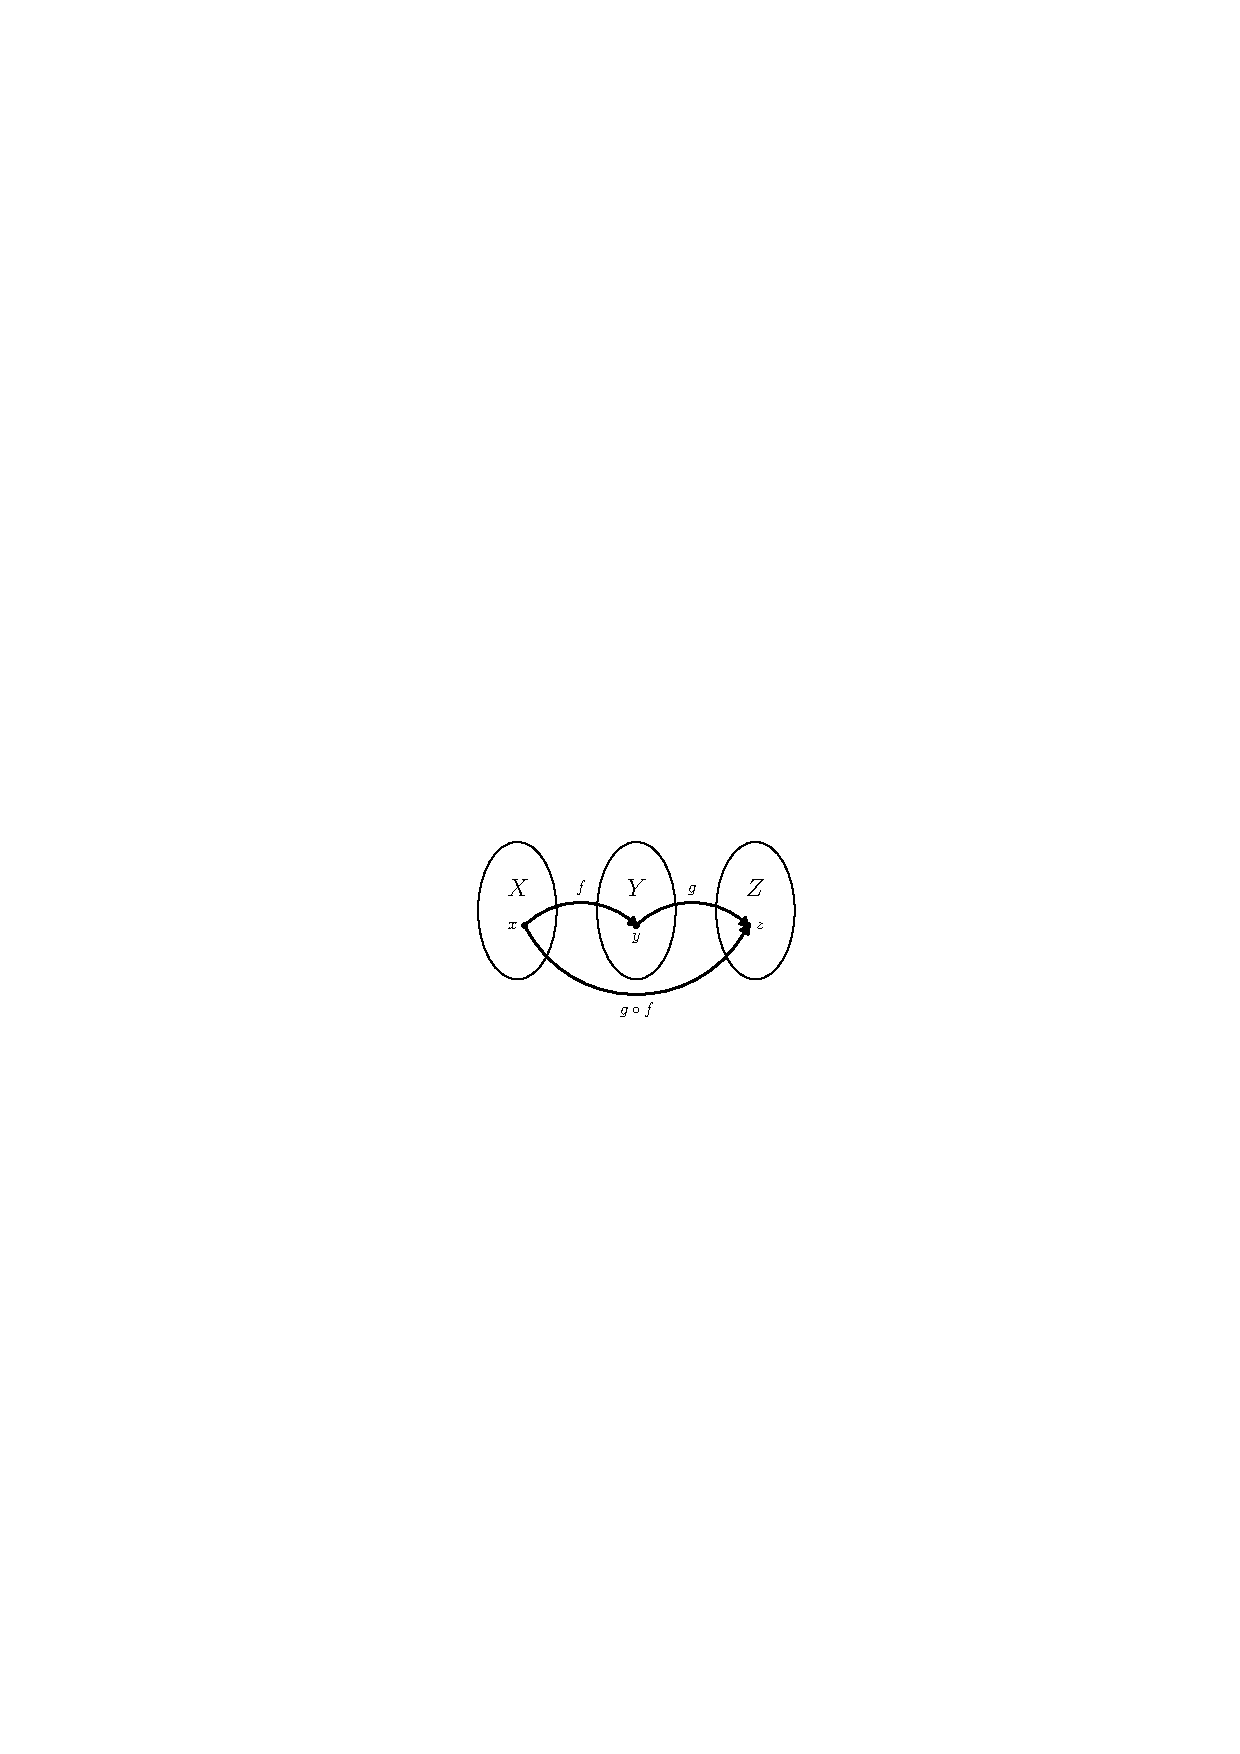
\includegraphics{graph/mapping-composition}
	\end{center}
\end{df}

Докажем два важных свойства композиций:

\begin{enumerate}
	\item Композиция биекций является биекцией.\index{отображение!биективное}
%		\begin{proof}
%			\emph{Стырить у кого-нибудь в лекции}
%		\end{proof}
	\item Ассоциативность композиций: $(g\circ f)\circ h=g\circ(f\circ h)$.
		\begin{proof}
			Рассмотрим левую часть:
			$$((g\circ f)\circ h)(x)\eqdef(g\circ f)(h(x))\eqdef g(f(h(x)))$$
			Рассмотрим правую часть:
			$$(g\circ(f\circ h))(x)\eqdef g((f\circ h)(x))\eqdef g(f(h(x)))$$
			Очевидно, что они равны.
		\end{proof}
\end{enumerate}

\paragraph{Бином Ньютона}\par\strut\\

\label{newton_binom}
\index{бином Ньютона}
\begin{multline*} (a+b)^n = \underbrace{(a+b)\times\dots\times(a+b)}_{\text{$n$ раз}} =\\= \underbrace{a^n+na^{n-1}b+\dots+\Cb_n^ka^{n-k}b^k+\dots+nab^{n-1}+b^n}_{\text{$2^n$ неприведенных слагаемых}}
\end{multline*}

Таким образом,
$$ (a+b)^n = \sum_{k=0}^{n} \Cb_n^k \times a^{n-k} \times b^k $$
$$ T_{k+1} = \Cb_n^k \times a^{n-k} \times b^{k} $$

\paragraph{Полиномиальная формула}\par\strut\\
\label{polynomial}
\index{полиномиальная формула}
Полиномиальная формула является обобщением бинома Ньютона.
\begin{multline*}
 \left(a_1 + \dots + a_k\right)^n = \sum_{i_1+\dots+i_k=n} \frac{n!}{i_1! \times \dots \times i_k!} \times (a_1^{i_1} \times \dots \times a_k^{i_k}) \\\text{или}\\
 \left(\sum_{j=1}^{k} a_j \right)^n = \sum_{ (\sum_{j=1}^{k} i_j) = n }\left( \frac{n!}{ \prod_{j=1}^{k} i_j! } \times \prod_{j=1}^{k} a_{j}^{i_j} \right)\end{multline*}
Число неподобных членов в разложении равно $\tilde{\Cb_k^n}=\Cb_{n+k-1}^k$ (получается, если представить $n$ ячеек, в которые необходимо расставить с повторениями цифры от $1$ до~$k$). 

\paragraph{Подсчёт числа отображений и подмножеств.}\par\strut\\

Используя принципы комбинаторики можно выяснить, что если $|X|=n, |Y|=m$, то:

\begin{enumerate}
  \item $|P(X)|$ -- количество всех подмножеств множества -- равно $2^n$.
  \item Число всех $m$-элементных подмножеств в $X$ равно $\Cb^m_n$.
  \item Число всех отображений из $X$ в $Y$ равно $m^n$
  \item Число всех сюръективных отображений из $X$ в $Y$ называется числом Стирлинга 2-го рода и вычисляется по формуле 
  $$S(n,m) = \frac{\sum\limits_{k=0}^m (-1)^k \Cb_m^k (m-k)^n}{m!}$$

    Прочитать об этом можно здесь: 
    \begin{enumerate}
      \item \href{http://mathworld.wolfram.com/StirlingNumberoftheSecondKind.html}{http://mathworld.wolfram.com/StirlingNumberoftheSecondKind.html}
      \item \href{http://ndp.jct.ac.il/tutorials/Discrete/node81.html}{http://ndp.jct.ac.il/tutorials/Discrete/node81.html}
    \end{enumerate}
  \item Число всех инъективных отображений из $X$ в $Y$ равно $m(m-1)\dots(m-n+1)\bw=\Cb^m_n\cdot m!\bw=\Ab^m_n$
  \item Число всех биективных отображений из $X$ в $X$ равно $n!$
\end{enumerate}

\section{Перестановки}
\label{permutation}

\epigraph{There's no sense in being precise when you don't even know what you're talking about.}{John von Neumann}

\subsection{Группа перестановок}
\index{группа!перестановок}

\begin{df}
  \emph{Отображение} -- правило, которое каждому 
  элементу из множества $\Xb$ ставит в соответствие некоторый элемент множества $\Yb$. 
\end{df}

%Основные типы отображений:
%\begin{enumerate}
% \item Сюръективное отображение.
%   $$\mathbf F\colon A\rightarrow  B,\spc\forall y\in \mathbf B\spc\exists x\in\mathbf A: y=F(x)$$
% \item Инъективное отображение.
%   $$F(x_1) = F(x_2) \ra x_1 = x_2$$
% \item Биективное отображение, или взаимооднозначное соответствие. Определяется как отображение, обладающее предыдущими двумя признаками.
%\end{enumerate}

Под перестановками на множестве понимаются биективные отображения множества в себя. Рассмотрим множество, состоящее из конечного числа элементов. Занумеруем их от 1 до n. Множество всех биективных отображений из $(1,2,\dots n)$ в себя обозначим через $S_n$, $|S_n|=n!$. Всякую из таких перестановок можно записать в виде таблицы

$$\sigma =\left(\begin{array}{cccc}1&2&\dots&n\\i_1&i_2&\dots& i_n\end{array}\right),$$
которая означает, что при выполнении такого отображения элемент с номером 1 переходит в элемент с номером $i_1$ и т.п.

Перестановки не обладают свойством коммутативности, но обладают свойством ассоциативности. Существование единичной и обратной перестановки гарантируют нам то, что множество всех перестановок $S_n$ является \emph{группой}.

Условимся перемножать перестановки справа налево.

\begin{df}%
\index{цикл}
\emph{Цикл}~--- перестановка, такая что $\alpha_1 \rightarrow \alpha_2 \rightarrow \dots \rightarrow \alpha_k \rightarrow \alpha_1$, $\alpha_1,\alpha_2\dots\alpha_k \in \{1,2,\dots n\}$. Обозначается $(\alpha_1,\alpha_2,\dots \alpha_k)$. 

Если при выполнении какой-то циклической перестановки элементы множества переходят сами в себя, то они называются неподвижными, иначе -- перемещаемыми. Два цикла называются независимыми, если у них нет общих перемещаемых элементов. Два независимых цикла коммутативны.
\end{df}

\begin{theorem}
Всякая перестановка представима в виде произведения независимых циклов.
\end{theorem}

\begin{df}%
\index{транспозиция}
\emph{Транспозиция} -- цикл длины 2, или изменение мест двух элементов между собой.
\end{df}

\begin{note}
  Любой цикл длины $k$ представим в виде произведения $k-1$ транспозиций:
  $$ (k_1,k_2\dots,k_n) = (k_1,k_n)\dots(k_1,k_3)(k_1,k_2)=(k_1,k_2)(k_2,k_3)\dots(k_{n-1},k_n) $$
\end{note}
\begin{note}
  Число циклов длины $k$ в $S_n$ равно $\Cb_n^k \cdot(k-1)!$
\end{note}

\begin{df}\index{перестановка!декремент}
  \emph{Декрементом} подстановки называется сумма длин независимых
  циклов в её разложении, уменьшенных на 1:
  $d=d(\sigma)=\sum\limits_{i=1}^s(k_i-1)$. Легко понять, что
  $\sgn\sigma=(-1)^d$.
\end{df}

\newpage
\subsection{Чётность, знак перестановки}

\begin{df}
  Назовём пару элементов $(i,j)$ \emph{правильной}, если $i\bw<j\ra\sigma(i)\bw<\sigma(j)$ и \emph{неправильной} в обратном случае. Чётностью\index{перестановка!чётность} перестановки будет называть чётность количества неправильных пар $k$ в этой перестановке. Знак\index{перестановка!знак} перестановки $\sgn\sigma\eqdef(-1)^k$.
\end{df}

\begin{note}
  Транспозиция меняет знак перестановки. При умножении перестановок из знаки также перемножаются: $\sgn(\pi\sigma)=\sgn\pi\cdot\sgn\sigma$.
\end{note}

\begin{note}
  Число чётных перестановок равно числу нечётных и равно $n!/2$.
\end{note}

\begin{df}
	$\Ab_n\subset\Sb_n=\{\sigma\vert\sgn\sigma>0\}$~--- подгруппа, называемая \emph{знакопеременной
	группой перестановок}\index{перестановка!знакопеременная}.
\end{df}

\section{Алгебраические структуры}
\label{groups}

\newcommand{\mnod}[2]{\left( #1 ; #2 \right)}
\newcommand{\mnok}[2]{\left[ #1 ; #2 \right]}

\epigraph{It is not enough to have a good mind; the main thing is to use it well.}{Rene Descartes}

\subsection{Полугруппы}

\begin{df}
  Пусть $\Gb$ -- некоторое множество. Тогда \emph{бинарной операцией}\index{операция!бинарная} на этом множестве будет называться правило, согласно которому каждой упорядоченной паре $(a,b)$, $a,b\in\Gb$, ставится в соответствие некоторый элемент $c\in\Gb$. Операция называется \emph{частичной}\index{операция!частичная}, если она определена не для всех пар.
\end{df}

\begin{df}
  Операция называется \emph{ассоциативной}\index{операция!ассоциативная}, если $\forall a,b,c\in\Gb$ $(ab)c\bw=a(bc)$. Множество, на котором задана ассоциативная операция, называется \emph{полугруппой}\index{полугруппа}. В случае ассоциативной операции значение выражения вообще не зависит от расстановки скобок:
\end{df}
\begin{note}
 В случае частичной бинарной операции следует сказать, что закон ассоциативности состоит в следующем: если определено хотя бы одно из произведений $a(bc)$ или $(ab)c$, то второе также определено и они равны.
\end{note}

\begin{theorem}[обобщённый закон ассоциативности]
  Произведение $n$ элементов в полугруппе не зависит от способа расстановки скобок.
\end{theorem}
\begin{proof}
  Проведём доказательство индукцией по $n$. База индукции -- $n=3$ -- известно.

  Теперь пусть $n\ge4$ фиксировано и известно, что для произведения меньшего чем $n$ числа элементов утверждение теоремы верно. Выделим скобки, над которыми производится последняя операция: $(a_1\cdot\dots\cdot a_k)\cdot(a_{k+1}\cdot\dots\cdot a_n)$. Назовём такую расстановку скобок расстановкой типа $k$. Внутри каждой из них возможна любая расстановка скобок по предположению индукции.

  Нам надо доказать, что для любой расстановки типа $m$, где $1\le m\le n-1$ произведение определено и результат одинаков. Для этого нам дано, что для некоторой расстановки типа $k$ это произведение определено.

  Достаточно показать, что определены произведения для расстановок типа $k\pm1$ тоже определены и результат одинаков во всех трёх случаях. Покажем, например, переход от $k$ к $k-1$:
  $$((a_1\cdot\dots\cdot a_{k-1})\cdot a_k)\cdot(a_{k+1}\cdot\dots\cdot a_n)=(a_1\cdot\dots\cdot a_{k-1})\cdot(a_k\cdot(a_{k+1}\cdot\dots\cdot a_n))$$

  Нетрудно заметить, что доказательство на этом завершается.
\end{proof}

\begin{df}
  Пусть $\Gb$ -- множество с бинарной операцией. Элемент $e\in\Gb$ называется \emph{левой единицей}, если $ea=a\cln\forall a\in\Gb$. Определение \emph{правой единицы}\index{единица} аналогично. Если в $\Gb$ имеется левая единица $e_1$ и правая единица $e_2$, то они совпадают и элемент $e=e_1=e_2$ называется (двусторонней) единицей.
\end{df}
\begin{df}
  Пусть $(\Gb,\cdot)$ обладает единицей. Тогда для элемента $a$ элемент $a'$ называется \emph{левым} (соответственно \emph{правым}) \emph{обратным}\index{элемент!обратный}, если $a'a=e$ ($aa'=e$). Также определяется двусторонний обратный элемент, который обозначается как $a^{-1}$. Элемент, имеющий обратный, называется \emph{обратимым}.\index{элемент!обратимый}
\end{df}
\begin{theorem}
  Если элемент обладает левым обратным и правым обратным, то они равны между собой.
\end{theorem}
\begin{note}
  На экзамене необходимо проиллюстрировать примерами все эти свойства. %\nota{Чего только не необходимо сделать на экзамене...}
\end{note}

\begin{df}
  По определению $a^n=a\cdot\dots\cdot a$ ($n$ раз), $a^0=e$, $a^{-n}=(a^{-1})^n\bw=(a^n)^{-1}$.
\end{df}
\begin{df}
  Элементы $a,b\in\Gb$ называются \emph{коммутирующими}, если $ab\bw=ba$. Если это выполнено для любых элементов, то операция (множество с этой операцией) называется коммутативной.\index{операция!коммутативная}
\end{df}

\subsection{Группы}

\begin{df}
 \emph{Группа}~--- множество с операцией, удовлетворяющее условиям:
\index{группа}%
 \begin{enumerate}
  \item Ассоциативность
  \item $\exists e\colon\cln ae=ea=a$
  \item $\forall a\cln\exists b\colon\cln ab = ba = e$. Обозначается $b = a^{-1}\cln(a = b^{-1})$
 \end{enumerate}
\end{df}

\begin{df}
Порядком элемента $a$ в группе называется наименьшее $n \in \mathbb N $, такое что $a^n = e$. Обозначается o(a) = n. Если $\nexists o(a)$, то принято считать, что $o(a) = \infty$.\index{порядок!элемента группы}
\end{df}

Порядок элемента группы отвечает следующему свойству:

\begin{theorem}
Пусть $o(a)=n$. Тогда $o(a^k)=\frac{n}{(k,n)}$
\end{theorem}
\begin{proof}
  Пусть $m$ -- положительное число такое, что $(a^k)^m\bw=e$. Значит $n\mid km$. Поэтому $m$ -- наименьший такой показатель, когда $km$~--- наименьшее общее кратное чисел $k$ и $n$, т.е. $km=\frac{kn}{(k,n)}\ra m=\frac{n}{(k,n)}$.
\end{proof}

\begin{theorem}
  \label{group:chaos}
  Порядок любого элемента конечной группы является делителем порядка группы (под порядком множества понимается количество его элементов).\index{порядок!группы}
\end{theorem}
\begin{proof}
  Пусть $|\Gb|=n$ и $a_1,\dots a_n$ -- её элементы. Пусть порядок произвольного элемента $a\in\Gb\cln o(a)=k$. Рассмотрим такое отображение $\pi_a\colon \pi_a(a_i)\bw=aa_i$. Это отображение биективно, следовательно может быть рассмотрено как перестановка на множестве $\Gb$. Разложим её в произведение независимых циклов. Каждый из циклов имеет вид $(a_i,aa_i,\dots a^{k-1}a_i)$ так как $a^la_i\ne a_i$ при $1\le l<k$; таким образом, если их число равно $m$, то $km=n$.
\end{proof}

\subsection{Кольца}

\begin{df}
  Если на множестве $K$ задано две операции (условно <<$+$>> и <<$\cdot$>>) и выполнены следующие условия:\index{кольцо}
  \begin{enumerate}
    \item $(K,+)$ -- абелева (коммутативная) группа\index{группа!абелева}
    \item $(K,\cdot)$ -- полугруппа
    \item $a(b+c)=ab+ac$ и $(a+b)c=ac+bc$,
  \end{enumerate}
  то $(K,+,\cdot)$ называется \emph{кольцом}.

  Если в $(K,\cdot)$ существует единица ($1\ne0$), то $K$ называется кольцом с единицей. Кольцо называется коммутативным, если $\forall x,y\cln xy=yx$. Обратимость элементов в кольце зависит от свойств алгебраической структуры $(K,\cdot)$.
\end{df}

\begin{df}
  Элемент $a$ называется левым (правым, двусторонним) \emph{делителем нуля}, если $\exists b\ne0$ такой, что $ab=0$ ($ba=0$, $ab=ba=0$ соответственно).\index{делитель нуля}
\end{df}

\begin{df}
  \emph{Поле} -- коммутативное кольцо с $1\ne0$, в котором всякий ненулевой элемент обратим.\index{поле}
\end{df}

\subsection{Кольца вычетов по модулю $n$}

На множестве целых чисел введём отношение эквивалентности таким
образом, что два числа $a$ и $b$ будут считаться эквивалентными, если
$a\equiv b \mod n$. Все целые числа сгруппируются по классам
эквивалентности, множество этих классов будем обозначать как $\Zc/n$,
а сами классы обозначим как $[a]=\{x\mid x\equiv a \mod n\}$. На
множестве классов логично определить операции сложения и умножения как
$[a]+[b]=[a+b]$ и $[a][b]=[ab]$, но требует проверки корректность
такого определения, то есть чтобы результат не зависел от выбранных
представителей в каждом из классов. В данном случае это не составит
большого труда. Также тривиальны и остальные необходимые проверки,
которые должны нам показать, что множество классов вычетов с такими
операциями является коммутативным кольцом с
единицей.\index{кольцо!вычетов}

Также легко заметить, что элемент $[k]$ в $\Zc/n$ обратим в том и только том случае, если $(k,n)=1$. Так как кольцо вычетов конечно и коммутативно, то всякий неделитель нуля в нём обратим. Действительно, если $a$ -- неделитель нуля, то все элементы $ax$ различны, значит один из них равен $1$.

Далее, обозначим за $U(\Zc/n)$ группу всех обратимых элементов кольца $\Zc/n$. Порядок этой группы равен $\varphi(n)$. Кольцо $\Zc/n$ является полем тогда и только тогда, когда $n$ -- простое.

\begin{theorem}[обобщённая малая теорема Ферма]
  $(k,n)=1\ra k^{\varphi(n)}\equiv 1 \mod n$.\index{теорема!Ферма}
\end{theorem}
\begin{proof}
  Если $(k,n)=1$, то $[k]\subset U(\Zc/n)$. По теореме \ref{group:chaos} имеем, что $[k]^{\varphi(n)}=[1]$, что и требовалось доказать.
\end{proof}
\begin{note}
  В частном случае, когда $n$ -- простое, имеем, что почти все $k$ таковы, что $(k,n)=1$ и $\varphi(n)=n-1$, то есть $k^n\equiv k \mod n$.
\end{note}

\begin{df}
  \emph{Характеристикой поля} называется такое наименьшее неотрицательное число $n$, что $1+\dots+1 \text{\:($n$ раз)} = 0$ . В случае, если такое не выполняется ни при каком натуральном $n$, принято считать, что характеристика поля $\Char\Pb = 0$.\index{характеристика поля} Если $\Char\Pb=n$, то $n$ -- простое.
\end{df}

\subsection{Построение поля частных области целостности}

\begin{theorem}
\label{group:pole}\index{поле!частных}
Любое коммутативное кольцо с единицей и без делителей нуля вкладывается в поле.
\end{theorem}
\begin{proof}
Пусть $\Kb$ ~-- коммутативное кольцо без делителей нуля. Это означает, что
$$ab=0\ra (a=0)\vee(b=0)$$

Для доказательства построим некоторое множество, состоящее из элементов кольца $\Kb$, если данное множество с определёнными на нём операциями будет являться полем, и будет существовать вложение $\varphi\colon\cln\Kb\rightarrow \Fb$, то кольцо $\Kb$ будет вложено в это поле.

Рассмотрим множество пар $(a,b),\cln a,b\in\Kb,\cln b\ne0$. Пусть пары $(a,b)$ и $(c,d)$ эквивалентны, если $ad=bc$. Эквивалентные пары будем обозначать таким образом: $(a,b)\sim(c,d)$. Пусть $\Ab$ ~--- множество всех таких пар. Отождествим эквивалентные пары. Это значит, что $$(a,b)\sim(c,d)\cln\&\cln(c,d)\sim(u,v)\ra(a,b)\sim(u,v)$$

$\blacktriangleright$
$$
\left\{
\begin{array}{lll}
ad&=&bc\\
cv&=&du
\end{array}
\right.
\lra
\left\{
\begin{array}{lll}
adv&=&bcv\\
bcv&=&bdu
\end{array}
\right.
\ra adv=bdu \ra av=bu \blacktriangleleft
$$

Обозначим за $[(a,b)]$ класс всех пар $(a_i,b_i)$, эквивалентных между собой. Тогда пусть множество всех классов $\Fb=\{ [(a,b)] \mid (a,b)\in \Ab\}$. Докажем, что это множество с указанными ниже операциями является полем, и в него будет вложено исходное кольцо $\Kb$.

На множестве $\Fb$ определим сложение двух классов:
$$[(a,b)]+[(c,d)]=[(ad+bc,bd)]$$

Далее будем обозначать класс или как $[(a,b)]$, или как
$\frac{a}{b}$. Тогда определение сложения примет привычный вид
$\frac{a}{b}+\frac{c}{d}=\frac{ad+bc}{bd}$. Покажем, что класс суммы
остаётся неизменным при различном выборе складываемых пар в классах
слагаемых.


\begin{proof}
  Пусть $(a,b)+(c,d)=(ad+bc,bd),\cln(a',b')+(c',d') = (a'd'+b'c',b'd')$. Иначе,
  $$
  \left\{
  \begin{array}{lll}
    ab'&=&ba'\\
    cd'&=&dc'
  \end{array}
  \right.
  \lra
  \left\{
  \begin{array}{lll}
    ab'dd'&=&dd'ba'\\
    cd'bb'&=&dc'bb'
  \end{array}
  \right.
  $$

  Сложим оба равенства:
  $$ ab'dd'+cd'bb'= dd'ba'+dc'bb'$$
  $$(ad+cb)b'd'   =(d'a'+c'b')bd $$

  Последнее означает не что иное, как $(ad+bc,bd)\bw\sim(a'd'+b'c',b'd')$.
\end{proof}

Теперь определим операцию умножения двух классов как $\frac{a}{b}\times\frac{c}{d}=\frac{ac}{bd}$. Необходимо теперь доказать корректность умножения, то есть что при различном выборе пар в классах $\frac{a}{b}$ и $\frac{c}{d}$ класс их произведения будет оставаться неизменным. Это доказательство аналогично вышеприведённому для сложения.

Для определённых нами операций сложения и умножения проверим аксиомы поля.

\begin{enumerate}
 \item $\frac{a}{b}+\frac{c}{d}=\frac{c}{d}+\frac{a}{b}$ (по определению)
 \item $\left(\frac{a}{b}+\frac{c}{d}\right)+\frac{s}{t} = \frac{a}{b}+\left(\frac{c}{d}+\frac{s}{t}\right)$

   $\blacktriangleright$ Рассмотрим правую и левую части. Если мы их равносильными преобразованиям приведём к равным выражениям, то доказательство будет завершено.
   $$\left(\frac{a}{b}+\frac{c}{d}\right)+\frac{s}{t}=\frac{ad+bc}{bd}+\frac{s}{t}=\frac{adt+bct+sbd}{bdt}$$
   $$\frac{a}{b}+\left(\frac{c}{d}+\frac{s}{t}\right)=\frac{a}{b}+\frac{ct+ds}{dt}=\frac{adt+bct+sbd}{bdt}\blacktriangleleft$$

 \item Класс $[(0;a)]$ отождествим с нулём.
 \item $\forall\frac{a}{b}\cln\exists\frac{-a}{b}\colon\cln\frac{a}{b}+\frac{-a}{b}=0$
 \item $\left( \frac{a}{b}+\frac{c}{d} \right)\frac{s}{t}= \frac{a}{b}\frac{s}{t}+\frac{c}{d}\frac{s}{t}$
 \item $\frac{a}{b}\cdot\frac{c}{d}=\frac{c}{d}\cdot\frac{a}{b}$
 \item $\left(\frac{a}{b}\cdot\frac{c}{d}\right)\frac{s}{t}=\frac{a}{b}\left(\frac{c}{d}\cdot\frac{s}{t}\right)$
 \item Класс $[(a,a)]$ отождествим с единицей.
 \item Обратным к $\frac{a}{b}$ будет являться $\frac{b}{a}$.
\end{enumerate}

Таким образом мы показали, что $\Fb$ с определёнными нами операциями
является полем. $\Fb$ называется полем частных кольца $\Kb$.

Определим вложение $\varphi\colon\cln a\rightarrow\frac{ax}{x},\cln a\in\Kb,\:\frac{ax}{x}\in\Fb$.

Это вложение сохраняет операцию: $a+b\stackrel{\varphi}{\longrightarrow} [((a+b)x,x)] =[(ax+bx, x)]=[(ax,x)] + [(bx,x)]$ (аналогично проверяется для умножения) и разные элементы переходят в разные:

\begin{proof}
  Пусть $a \to \frac{ab}{b},\cln a'\to \frac{a'b}{b}$. Необходимо
  доказать, что при различных $a$ и $a'$, $\frac{ab}{b}$ и
  $\frac{a'b}{b}$ также не совпадают. Докажем от противного. Пусть
  $a\ne a',\cln \frac{ab}{b}=\frac{a'b}{b}$. Последнее выражение
  означает, что $(ab,b)\sim(a'b,b)$ или $abb=a'bb$. Так как исходное
  кольцо $\Kb$ без делителей нуля, то или $a=a'$, или $b=0$. Но мы
  определили классы в множестве $\Ab$ так, что $b\ne 0$. Следовательно
  $a=a'$. Противоречие.
\end{proof}

Таким образом, мы построили такое множество $\Fb$ из элементов $\Kb$ и определили на нём две операции таким образом, что множество с этими операциями является полем и показали такое отображение $\Kb \stackrel{\varphi}{\longrightarrow} \Fb$, что оно является вложением.
\end{proof}

\begin{ex}
Кольцо целых чисел $\mathbb Z$ вложено в поле рациональных чисел $\mathbb Q\colon\mathbb Z \subset \mathbb Q$
\end{ex}

\subsection{Понятие гомоморфизма и изоморфизма}

\begin{df}
Отображение $\varphi\colon (G,\cdot)\to(K,*)$ называется \emph{гомоморфизмом}, если оно <<сохраняет операцию>>, т.е. $f(a\cdot b)=f(a)*f(b)\cln\forall a,b\in G$.\index{гомоморфизм}
\end{df}

\begin{stm}
  Образ группы при гомоморфизме является группой. При этом $\varphi(e)\!\!\bw=e'$. Однако при гомоморфизме полугрупп образ единицы не обязательно является единицей.
\end{stm}

Гомоморфизм колец уже обязан сохранять обе операции. В общем случае, опять же, единица не обязательно переходит в единицу.

\begin{theorem}
  Пусть $\Pb$ -- поле и $\Kb$ -- кольцо. В таком случае если существует гомоморфизм $\varphi\colon\Pb\to\Kb$, то $\varphi$ либо тривиален, либо инъективен.
\end{theorem}
\begin{proof}
  Пусть $x\neq y$ и $f(x)=f(y)\ra f(x-y)=0$. В силу существования $(x-y)^{-1}$ имеем
  \begin{equation*}
    f(1)=f\hr{(x-y)(x-y)^{-1}}=0
  \end{equation*}
  то есть $\forall a\in\Pb\colon f(a)=f(a\cdot 1)=0$.
\end{proof}

\begin{df}
  Отображение $\varphi$ называется \emph{изоморфизмом}, если $\varphi$ является гомоморфизмом и $\varphi$ -- биективно. Два множества с алгебраическими операциями называются изоморфными, если существует изоморфизм, переводящий одно в другое.\index{изоморфизм}
\end{df}

\begin{theorem}[Кейли]\index{теорема!Кейли}
  Всякая группа порядка $n$ изоморфна некоторой подгруппе симметрической группы $S_n$.
\end{theorem}
\begin{proof}
  Пусть $\Gb=\{a_1,a_2,\dots,a_n\}$ -- группа порядка $n$. Составим для группы $\Gb$ таблицу Кейли и сопоставим каждому элементу $a_i\in\Gb$ перестановку на множестве $\Gb$, задаваемую $i$-й строкой таблицы Кейли, то есть рассмотрим отображение $f\colon \Gb\to S_n$, при котором $f(a)=\pi_a,\cln \pi_a(a_j)=aa_j$. Разным элементам группы $\Gb$ соответствуют разные перестановки, таким образом отображение $\Gb\to \Im f$ -- биективно.

  Докажем, что оно является гомоморфизмом. $\forall a_j\in\Gb$ имеем $\pi_{ab}(a_j)\bw=(ab)a_j\bw=a(ba_j)\bw=\pi_a(\pi_b(a_j))\bw=(\pi_a\circ\pi_b)(a_j)$.
\end{proof}

\begin{theorem}
  Пусть $\Pb$ -- поле. Имеется единственный инъективный гомоморфизм
    \begin{enumerate}
      \item $f\colon\Q\to\Pb$, если $\Char\Pb=0$;
      \item $f\colon \Zc/p\to\Pb$, если $\Char\Pb=p$.
    \end{enumerate}
  В обоих случаях $\Im f$ является единственным минимальным полем поля $\Pb$.
\end{theorem}
\begin{proof}
  \begin{enumerate}
    \item $\Char\Pb=0$. Тогда $\forall n\colon n\cdot1\ne0$. Зададим
      отображение $f$ по правилу
      $f\left(\frac{m}n\right)\bw=(m\cdot1)(n\cdot 1)^{-1}$. Так как
      запись рационального числа в виде дроби неоднозначна, то
      необходимо проверить, что легко сделать, что подобное задание
      $f$ корректно. Далее проверяем, что $f$ -- гомоморфизм, который
      является инъективным, так как $\Qb$ -- поле. Так как
      $f(1_\Q)=1_{\Pb}$, то $f$ определён однозначно.
    \item $\Char\Pb=p$. Определим $f([k])=k\cdot1$. Так как $o(1)=p$, то $k\cdot1=l\cdot1\lra k\equiv l\mod p$ и отображение определено корректно. Очевидно, что оно гомоморфизм, инъективно и однозначно.
  \end{enumerate}

  В обоих случаях $\Im f$ содержится в любом подполе $\Lb$ поля $\Pb$ так как $1\in\Lb$, а значит все элементы $n\cdot1\in\Lb$ и $(m\cdot1)(n\cdot)^{-1}\in\Lb\cln(1\cdot1\ne0)$. $\Im f$ называется \emph{простым подполем}\index{подполе простое} поля $\Pb$.
\end{proof}
\subsection{Циклические группы}

\begin{df}
Пусть $(\Gb,\cdot)$ -- группа и $a\in\Gb$. Тогда множество $\left\langle a\right\rangle=\{a^n\mid n\in\Zc\}$ называется \emph{циклической подгруппой} с \emph{порождающим элементом} $a$. Очевидно, что $|\left\langle a\right\rangle|=o(a)$. Может так оказаться, что $\left\langle a\right\rangle = \Gb$. В таком случае сама группа $\Gb$ называется циклической.\index{группа!циклическая}
\end{df}

Если $\left\langle a\right\rangle$ -- циклическая группа порядка $n$, то порядок элемента $o(a^k)=\frac{n}{(n,k)}$. Если $(n,k)=1$, то элемент $a^k$ является порождающим в этой группе. Легко понять, что число образующих в группе порядка $n$ равно $\varphi(n)$. Очевидно, что если группа простого порядка, то каждый элемент этой группы будет являться порождающим. Если $|\left\langle a\right\rangle|=\infty$, то образующими являются только элементы $a$ и $a^{-1}$.

\begin{theorem}
  Пусть $G=\left\langle a \right\rangle$ циклическая группа и $(K, \cdot)$ -- произвольная группа. В таком случае существует единственный гомоморфизм $f\colon G\to K,$ при котором $f(a)=b$ для любого $b$, если $|\left\langle a\right\rangle|=\infty$ и для $b\colon b^n=e$, если $|\left\langle a\right\rangle|=n$.
\end{theorem}
\begin{proof}
  Так как при гомоморфизме $f(a^k)=f^k(a)$, то $f$ однозначно задаётся своим значением $f(a)$. В случае бесконечной группы $G$ утверждение теоремы становится очевидным. В случае конечной, в общем-то, тоже.
\end{proof}

\begin{theorem}
  Две любые группы одного и того же простого порядка изоморфны между собой.
\end{theorem}

\subsection{Разложение группы на смежные классы. Теорема Лагранжа}

\begin{df}
  Пусть $H$ -- подгруппа в $\Gb$. Множества вида $gH = \{gh\mid h\in H\}$ при фиксированном $g\in\Gb$ называются \emph{левыми смежными классами} группы $\Gb$ по подгруппе $H$. Аналогично определяются правые смежные классы.\index{классы!смежные}
\end{df}

\begin{theorem}
  Каждый левый смежный класс определяется любым своим элементом, т.е. если $g'\in gH$, то $g'H=gH$. Два левых смежных класса либо не пересекаются, либо совпадают. Объединение всех левых смежных классов равно $\Gb$. Отображение $H\to gH$ биективно.
\end{theorem}
\begin{proof}
  Пусть $g'\in gH$, т.е. $g'=gh,\cln h\in H$. Тогда $g'H=ghH\subset gH$; так как $g=g'h^{-1}$, то $g\in g'H$ и $gH\subset g'H$, из чего следует $gH=g'H$. Остальные утверждения теоремы выводятся не менее просто.
\end{proof}

Разбиение множества $\Gb$ на попарно непересекающиеся классы равносильно введению отношения эквивалентности на этом множестве.

\begin{theorem}
  Два элемента $g_1,g_2\in\Gb$ принадлежат одному левому смежному классу по подгруппе $H$ тогда и только тогда, когда $g_1^{-1}g_2\in H$.
\end{theorem}
\begin{proof}
  $g_2\in g_1H \lra g_2=g_1h$ для некоторого $h\in H$. Следовательно, $g^{-1}g_2\in H$.
\end{proof}

\begin{theorem}
  Отображение $x\to x^{-1}$ группы $\Gb$ на себя задаёт биективное соответствие между множествами левых и правых смежных классов по подгруппе $H$.
\end{theorem}
\begin{proof}
  $$(gH)^{-1}=\{(gh)^{-1}\mid g\in H\} = \{h^{-1}g^{-1}\mid h\in H\}=\{hg^{-1}\mid h\in H\}=Hg^{-1}$$
\end{proof}

\begin{df}
  Число (левых или правых) смежных классов группы $\Gb$ по подгруппе $H$ называется \emph{индексом}\index{индекс подгруппы} подгруппы $H$ в $\Gb$ и обозначается $(\Gb:H)$.
\end{df}

\begin{theorem}[Лагранжа]\index{теорема!Лагранжа}
  Пусть $\Gb$ -- конечная группа. Тогда $|H|\cdot (\Gb:H)=|G|$.
\end{theorem}
\begin{proof}
  Если $|H|=d$, то для каждого элемента $h\in H$ имеем $(\Gb:H)$, например, левых смежных классов, которые не пересекаются между собой и при объединении дают $\Gb$. Таким образом утверждение теоремы очевидно.
\end{proof}

Примеры разбиения множества на смежные классы:
\begin{enumerate}
  \item $G=(\Zc,+),\cln H=n\Zc$. Получаемые таким образом классы называются \emph{классами вычетов}.
  \item $G=(\R,+),\cln H=2\pi\Zc$. Смежные классы $\al+2\pi\Zc$ находятся в биективном соответствии с с углами, которые образуют векторы на плоскости с положительным направление оси абсцисс.
  \item \dots
\end{enumerate}

\section{Векторная алгебра}
\label{vector}

\epigraph{He who seeks for methods without having a definite problem 
  in mind seeks in the most part in vain.}{David Hilbert}

\subsection{Основные понятия. Линейная комбинация векторов}

\begin{df}
  \emph{Вектор}\index{вектор} -- упорядоченный набор из чисел, называемых координатами вектора. Вектор -- элемент арифметического n-мерного \index{пространство}пространства $\R^n$. Над векторами определены следующие операции:
  \begin{enumerate}
    \item Сложение (означает почленное сложение его координат)
    \item Умножение на скаляр
  \end{enumerate}
\end{df}

Основные свойства операций:

\begin{enumerate}
  \item $\forall \ab,\bb\in\R^n\cln \ab+\bb=\bb+\ab$
  \item $\forall \ab,\bb,\cb \cln (\ab+\bb)+\cb=\ab+(\bb+\cb)$
  \item $\exists \mathbf 0\colon \ab+\mathbf 0=\ab;$
  \item $\forall \ab\cln\exists(-\ab)\colon \ab+(-\ab)=0$
  \item $\forall\al,\beta\in\R, \ab\colon (\al\beta)\ab=\al(\beta \ab)$
  \item $(\al+\beta)\ab=\al \ab+\beta \ab$
  \item $\al(\ab+\bb)=\al \ab+\al \bb$
  \item $\forall\ab\in\R^n\cln1\cdot\ab=\ab,\cln 0\cdot\ab=\mathbf 0$
\end{enumerate}

\begin{df}
  Пусть даны $\ab_1, \ab_2,\ab_3,\dots, \ab_m\in\R^n$ и $\al_1,\al_2,\dots\al_m\in\R$. Тогда выражение $\al_1\ab_1+\al_2\ab_2+\dots+\al_m\ab_m\in\R^n$ назовём \emph{линейной комбинацией}\index{линейная!комбинация} векторов $\ab_1, \ab_2,\dots, \ab_m$. Если $\al_1\ab_1+\al_2\ab_2+\dots+\al_m\ab_m=0$, то говорят, что задано \emph{линейное соотношение} этих векторов. Соотношение $0\cdot\ab_1+\dots+0\cdot\ab_m=0$ называется \index{соотношение!тривиальное}\emph{тривиальным}. \index{соотношение!нетривиальное}\emph{Нетривиальным} называется соотношение, в котором хотя бы один из коэффициентов не равен 0.
\end{df}
\begin{df}
  Под \emph{системой векторов} понимается индексированная совокупность векторов, т.е. в системе могут содержаться равные между собой вектора, но наделённые разными индексами.
\end{df}
\begin{df}
  Конечная система векторов называется \emph{линейно зависимой}\index{линейная!зависимость}, если для неё существует нетривиальное линейное соотношение. Если же существует только тривиальное линейное соотношение, то такая система называется \emph{линейно независимой}. Пустая система векторов линейно независима.
\end{df}
\begin{stm}
  Любая подсистема в линейно независимой системе линейно независима.
\end{stm}
\begin{stm}
  Система линейно зависима тогда и только тогда, когда хотя бы один вектор этой системы выражается через остальные.
\end{stm}
\begin{stm}
  Если какая-то подсистема системы зависима, то и вся система линейно зависима. \emph{Другими словами, любую линейно зависимую систему можно расширить}.
\end{stm}
\begin{stm}
  Если система векторов линейно зависима, то и система укороченных
  векторов линейно зависима.
\end{stm}
\begin{stm}
  В пространстве $\R^n$ всякая система, содержащая больше, чем $n$ векторов, линейно зависима.
\end{stm}
\begin{df}
  Говорят, что вектор $\bb$ линейно выражается через систему векторов $\{\ab_i\}$, если $\exists\al_1,\dots\al_n\colon \bb=\sum\limits_i \al_i\ab_i$.

  Говорят, что система $\Sb\subset\R^n$ линейно выражается через систему $\Tb\subset\R^n$, если каждый вектор из $\Sb$ линейно выражается через конечную подсистему в $\Tb$. Две системы векторов называются 
\emph{эквивалентными}, если каждая из них линейно выражается через другую.
\end{df}

\begin{theorem}[Основная лемма о линейной зависимости]
  \label{mainlemma}\index{лемма!о линейной зависимости}
  Пусть даны системы векторов $\Ab=\{\ab_1,\dots,\ab_m\},\Bb=\{\bb_1,\dots,\bb_k\}\in\R^n$ и система $\Bb$ линейно выражается через $\Ab$. Тогда если $k>m$, то $\Bb$ линейно зависима.
\end{theorem}
\begin{proof}
  Имеем систему уравнений:
  $$
   \left\{
    \begin{array}{rcl}
      \bb_1 &   =   & \sum\limits_i^m\al_{1i}\ab_i\\
          & \dots & \\
      \bb_k &   =   & \sum\limits_i^m\al_{ki}\ab_i\\
    \end{array}
   \right.
  $$
  
  Рассмотрим систему векторов $\{\mathbf\lambda_j\}$, в которой i-й вектор будет иметь координаты $(\al_{i_1},\dots\al_{i_m})$. Система этих векторов обязательно линейно зависима, потому что количество векторов в ней больше размерности пространства, которому они принадлежат. Таким образом мы всегда можем выбрать коэффициенты $\{ \mu_j \}$, так, чтобы $\sum_j^k \mu_j\mathbf\lambda_j = 0$. Понятно, что если мы возьмём линейную комбинацию $\sum_j^k \mu_j \bb_j$, то она тоже окажется равной 0. Теорема доказана.
\end{proof}
\begin{note}
  \emph{Другая формулировка этой леммы такова: <<Линейно независимую систему систему нельзя выразить через меньшее количество векторов, чем она содержит>>}.
\end{note}

\subsection{Базис системы векторов}\index{базис!системы векторов}

\begin{df}
  Пусть $\Sb\subset\R^n$ -- любая система векторов. Набор векторов $\ab_1,\dots \ab_r$ называется \emph{базисом} системы $\Sb$, если
  \begin{enumerate}
    \item $\ab_1,\dots \ab_r$ линейно независимы.
    \item $\forall \bb\in\Sb$ линейно выражается через $\ab_1,\dots \ab_r$.
  \end{enumerate}
\end{df}

\begin{stm}
  Базис -- максимальная линейно независимая подсистема. Всякую линейно
  независимую систему в $\Sb$ можно дополнить до базиса $\Sb$.
\end{stm}

\begin{stm}
  Любая система $\Sb\subset\R^n$ имеет базис. Стандартным базисом для $\R^n$ называется система векторов вида $\eb_i = (\underbrace{0,\dots,0}_{i-1},1,\underbrace{0,\dots,0}_{n-i})$\index{базис!стандартный}
\end{stm}

\begin{theorem}
  Любые 2 базиса $\Ab$ и $\Bb$ системы содержат равное количество векторов.
\end{theorem}
\begin{proof}
  Пусть подсистемы $\Ab = \{a_1\dots,a_n\}$ и $\Bb=\{b_1,\dots,b_m\}$
  являются базисами, тогда каждая из них линейно выражается через
  другую. По основной лемме о линейной зависимости (\ref{mainlemma})
  имеем, что $m\le n $ и $m\ge n$, т.е. $m=n$.
\end{proof}

\begin{df}
  \emph{Рангом}\index{ранг!системы векторов} системы векторов называется число векторов любом её базисе. Обозначается $\rk\Sb = r$. Например, $\rk\R^n=n$.
\end{df}

\begin{theorem}
  Конечная подсистема $(a_1,\dots, a_r)$ системы векторов $\ab$ является базисом её базисом в том и только том случае, если всякий вектор из $\ab$ выражается через $(a_1,\dots, a_r)$ единственным образом.
\end{theorem}
\begin{proof}
  Докажем необходимость и достаточность:
  \begin{itemize}
    \item[($\Leftarrow$)]  Пусть $(a_1,\dots, a_r)$ -- базис и допустим, что имеются два представления какого-то вектора $b\in\ab$:
    \begin{gather*}
     b=\lambda_1a_1+\lambda_ra_r\\
     b=\lambda_1'a_1+\lambda_r'a_r
    \end{gather*}
    Тогда $0=b-b=(\lambda_1-\lambda_1')a_1+(\lambda_r-\lambda_r')a_r\ra\forall i\colon\lambda_i=\lambda_i'$ так как $(a_1,\dots, a_r)$ линейно независима и для неё может существовать только тривиальная линейная комбинация.
    
    \item[($\Rightarrow$)] Предположим, что векторы из $\ab$ единственным образом выражаются через систему $(a_1,\dots, a_r)$. Чтобы установить, что подсистема $(a_1,\dots, a_r)$ является базисом, нужно показать, что $(a_1,\dots, a_r)$ -- линейно независима. Допустим обратное, т.е. имеется линейное соотношение
    $$\alpha_1a_1+\dots+\al_ra_r=0.$$
    Рассмотрим представление какого-то вектора $b\in\ab$:
    $$b=\lambda_1a_1+\dots+\lambda_ra_r$$
    В силу единственности представления вектора $b$ в виде линейной комбинации векторов $a_1,\dots, a_r$ получаем, что $\forall i\colon\lambda_i=\lambda_i+\al_i\ra \al_i=0$, т.е. $(a_1,\dots, a_r)$ линейно независима.
  \end{itemize}
\end{proof}

\begin{stm}
  Если $\Bb$ линейно выражается через $\Ab$, то $\rk \Bb\le\rk\Ab$. \emph{(Доказательство проводится по основной лемме о линейной зависимости (\ref{mainlemma}))}
\end{stm}

\subsection{Подпространства в $\R^n$}\index{пространство!подпространства}

\begin{df}
  Подмножество $\Lb\subset \R^n$ называется подпространством, если
  \begin{enumerate}
    \item $\Lb\ne\emptyset$
    \item $a,b\in\Lb\ra a+b\in\Lb$
    \item $a\in\Lb\ra \forall\lambda\in\R\cln\lambda a\in\Lb$
  \end{enumerate}
\end{df}

\begin{df}
  \index{плоскость}Плоскость в n-мерном пространстве есть множество векторов, полученное сдвигом какого-то подпространства на несущий вектор.
\end{df}

  \begin{df}
  Пусть имеется какая-то система векторов $\mathbf S=(a_1\dots a_s)\in\R^n$. Тогда множество всех линейных комбинаций векторов из $\mathbf S$ называется линейной оболочкой множества $\mathbf S$ и обозначается $<\!\mathbf S\!>$.
  $$<\!\mathbf S\!>=<a_1,\dots, a_r>=\{ \lambda_1a_1+\lambda_2a_2+\dots+\lambda_sa_s\mid\forall \lambda_i\in\R\}$$
  Линейная оболочка пустого множества $<\!\emptyset\!>$ равна нулевому вектору.\index{линейная!оболочка}
  \end{df}
  
  Сформулируем несколько следствий из определения:
  \begin{itemize}
    \item Линейная оболочка любого множества является подпространством
    \item Всякое подпространство является линейной оболочкой своего базиса.
    \item Условие, что система векторов $\bb$ линейно выражается через систему векторов $\ab$, равносильно тому, что $<\!\bb\!>\,\subseteq\,<\!\ab\!>$.
    \item Две системы векторов эквивалентны тогда и только тогда, когда из линейные оболочки совпадают.
  \end{itemize}
  
  Задание подпространства линейной оболочкой какой-либо системы векторов является только одним из возможных вариантов. Вторым способом является задание подпространства множеством решений ОСЛУ (см. \ref{oslu}). В данном случае можно, конечно, считать, что подпространство задаётся линейной оболочкой её фундаментальной системы решений\index{фундаментальная система решений} (далее: ФСР).
  
  \begin{df}
    В случае разговора о подпространствах, вместо термина <<ранг>>\index{ранг!подпространства} подпространства употребляют термин \index{размерность}<<размерность>> подпространства. Обозначается $\dim \Lb$. Размерность подпространства равна его рангу как системы векторов.
  \end{df}

\section{Матрицы}
\label{matrix}

\epigraph{Errors using inadequate data are much less than those using
  no data at all.}{Charles Babbage}

\subsection{Основные понятия}

\begin{df}
  \emph{Матрица}\index{матрица} -- прямоугольная таблица из чисел или любых других объектов.
  $$
  A =
  \begin{pmatrix}
   a_{11}&a_{12}&\dots&a_{1n}\\
   a_{21}&a_{22}&\dots&a_{2n}\\
   \vdots&\vdots&\ddots&\vdots\\
   a_{n1}&a_{n2}&\dots&a_{mn}
  \end{pmatrix}
  $$
\end{df}

Над матрицами определены следующие операции:
\begin{enumerate}
\item Умножение на скаляр.
\item Транспонирование.\index{матрица!транспонированная} Строки
  записываются в столбцы. Обозначается $A^T$
\item Сложение матриц. Определено только для матриц одинакового
  размера, производится почленное сложение всех элементов матрицы.
\item Умножение матриц. Определяется следующим способом: пусть даны
  матрицы $A$ размером $m\times n$ и $B$ размером $n\times k$. Тогда
  матрица $C=AB$ будет состоять из элементов
  $c_{i_j}=\sum\limits_{k=1}^n a_{i_k}b_{k_j}$. 
\end{enumerate}
  
Так как матрицы являются обобщением векторов, то операциям сложения и
умножения на скаляр соответствуют все заявленные для векторов 8
свойств, некоторые другие свойства теории линейной зависимости также
сохраняются.
  
Можно также доказать следующие свойства, относящиеся к вновь определённым операциям:
\begin{enumerate}
\item $(A+B)^T = A^T+B^T$
\item $(A+B)C=AC+BC$
\item $A(BC)=(AB)C$
  \begin{proof}
    Определим сначала базис пространства матриц $M_{m\times
      n}(\R)$. Он будет состоять из \emph{матричных
      единиц}\index{матричная единица} $E_{ij}$ \emph{(на
      пересечении i-й строки и j-го столбца стоит 1, а все
      остальные элементы равны 0}. Всякая матрица будет
    представима в виде линейной комбинации матричных единиц.
    
    Теперь осталось проверить только ассоциативность умножения
    матричных единиц. В общем
    случае 
    \begin{displaymath}
      E_{ij}E_{kl}=\left\{\begin{array}{ll}E_{il}, &   k=j\\0,&k\ne j\end{array}\right..
    \end{displaymath}
    Легко проверяется, что
    умножение матричных единиц ассоциативно. Из этого следует, что
    и умножение любых матриц ассоциативно, так как ранее мы
    доказали свойство дистрибутивности.
  \end{proof}
\item $(AB)^T=B^TA^T$
\end{enumerate}

\begin{df}
  \emph{Следом}\index{след матрицы} матрицы $\tr A$ называется сумма диагональных элементов матрицы. 
  %Можно заметить, что для этой функции существует ряд очень интересных свойств, 
  % о которых, может быть, будет рассказано позднее.
\end{df}
  
Докажем следующее важное свойство: $\tr(AB)=\tr(BA)$:
\begin{proof}
  Проведём доказательство одной строкой:
  $$\tr(AB)=\sum_i\sum_k a_{ik}b_{ki}=\sum_k\sum_i a_{ik}b_{ki}=\sum_k\sum_i b_{ki}a_{ik}=\tr(BA)$$%
\end{proof}

\begin{df}
  Единичной матрицей\index{матрица!единичная} называется такая матрица $E$, что $AE\bw=EA\bw=A$. Такая матрица имеет следующий вид (все элементы, кроме элементов главной диагонали, равны нулю):
  \begin{center}
    \scalebox{0.7}{
      $
        A =
        \begin{pmatrix}
          1&0&\dots&0\\
          0&1&\dots&0\\
          0&0&\ddots&\vdots\\
          0&0&\dots&1
        \end{pmatrix}
      $
    }
  \end{center}
\end{df}
  
\begin{df}
  Если в строке матрицы все элементы -- нули, то такая строка
  называется \emph{нулевой}. Первый ненулевой элемент в строке
  называется \emph{главным} или \emph{лидером}.
\end{df}
  
\begin{df}
  \emph{Элементарными преобразованиями (далее: ЭП) строк
    матрицы}\index{элементарные преобразования} называются
    преобразования вида:
  \begin{enumerate}
  \item К i-й строке прибавить j-ю, умноженную на $\lambda\in\mathbb R$
  \item Поменять местами i-ю и j-ю строки
  \item Умножить i-ю строку на $\lambda\ne0$
  \end{enumerate}
  Элементарные преобразования строк или столбцов матрицы можно
  записать как произведение исходной матрицы на одну из
  \emph{элементарных матриц}\index{элементарные матрицы} (прямых или
  транспонированных). Если матрицу умножить на одну из элементарных
  матриц слева ($A'=E_iA$), то соответствующее преобразование затронет
  строки, если справа -- столбцы.
  
  
  \begin{center}
    \scalebox{0.75}{
  $
    E_1 =
  \begin{pmatrix}
   1&      & &       &       &      & \\
    &\ddots& &       &       &      & \\
    &      &1&\dots  &\lambda   &\dots & \\
    &      & &\ddots &       &      & \\
    &      & &       &\ddots &      & \\
    &      & &       &       &1     &
  \end{pmatrix}\spc
  $
  }
  \scalebox{0.5}{
  $
  E_2 =
  \begin{pmatrix}
   1&      & &      & &      & &      & \\
    &\ddots& &      & &      & &      & \\
    &      &0&      & &      &1&      & \\
    &      & &\ddots& &      & &      & \\
    &      & &      &1&      & &      & \\
    &      & &      & &\ddots& &      & \\
    &      &1&      & &      &0&      & \\
    &      & &      & &      & &\ddots& \\
    &      & &      & &      & &     &1
  \end{pmatrix}
  \spc
  $
  }
  \scalebox{0.65}{
  $
    E_3 =
  \begin{pmatrix}
   1&      & &       & &      & \\
    &\ddots& &       & &      & \\
    &      &1&       & &      & \\
    &      & &\lambda& &  &      & \\
    &      & &       &1&      & \\
    &      & &       & &\ddots& \\
    &      & &       & &      &1\\
  \end{pmatrix}
  $
  }
  \end{center}
\end{df}

\newpage
\begin{df}
  Матрица называется ступенчатой\index{матрица!ступенчатая}, если она удовлетворяет следующим условиям:
  \begin{enumerate}
     \item Ниже нулевой строки (если она есть) находятся только нулевые строки
     \item В каждой ненулевой строке её лидер стоит строго правее, чем в предыдущей.
  \end{enumerate}
  %% FIXME: Bug somewhere here, but I am too asleep to fix it.
  %% \begin{center}
  %%   \scalebox{0.7}{
  %%     $
  %%     \tilde A' =
  %%     \left(
  %%     \begin{array}{c}
  %%       \begin{array}{m{3mm}|m{3mm}m{3mm}m{3mm}m{3mm}m{3mm}m{3mm}|m{3mm}}
  %%         &*& . & . & . & . & . & .\\
  %%         \cline{2-2}
  %%       \end{array}\\
  %%       \begin{array}{m{3mm}m{3mm}|m{3mm}m{3mm}m{3mm}m{3mm}m{3mm}|m{3mm}}
  %%         & & * & . & . & . & . & .\\
  %%         \cline{3-4}
  %%       \end{array}\\
  %%       \begin{array}{m{3mm}m{3mm}m{3mm}m{3mm}|m{3mm}m{3mm}m{3mm}|m{3mm}}
  %%      & &   &   & * & . & . & .\\
  %%         \cline{5-8}
  %%       \end{array}\\
  %%       \begin{array}{m{3mm}m{3mm}m{3mm}m{3mm}m{3mm}m{3mm}m{3mm}|m{3mm}}
  %%         &0&   &   &   &   &   & .\\
  %%       \end{array}\\
  %%   \begin{array}{m{3mm}m{3mm}m{3mm}m{3mm}m{3mm}m{3mm}m{3mm}|m{3mm}}
  %%     & &   &   &   &   &   &  \\
  %%   \end{array}\\
  %%     \end{array}  
  %%     \right)
  %%     $
  %% }
  %% \end{center} 
\end{df}
  
\begin{theorem}
  Любую матрицу можно привести к ступенчатому виду используя только ЭП 1 типа.
  \label{mat:echelon}
\end{theorem}
  
\begin{proof}
  Докажем теорему при помощи метода математической индукции. Индукцию
  проведём по количеству строк матрицы.
  
  Для $m = 1$ утверждение верно, так как матрица, состоящая из одной строки ступенчатая.
    
  Для удобства будем рассматривать матрицу без нулевых
  столбцов. Рассмотрим матрицу из m строк и её первую строку. Возможно
  две ситуации:
  \begin{enumerate}
  \item $a_{11}\ne0$. Тогда с помощью ЭП 1 типа мы можем сделать все остальные элементы этого столбца нулевыми, добавив к каждой (i-й) строке этой матрицы первую, умноженную на $-\frac{a_{i1}}{a_{11}}$. 
  \item $a_{11}=0$. Так как мы исключили из рассмотрения все нулевые столбцы, то существует ненулевой элемент в первом столбце. Добавим к первой строке строку, содержащую этот элемент и реализуем алгоритм, описанный в пункте 1.
  \end{enumerate}
    
    По предположению индукции подматрицу этой матрицы из $m-1$ строки (со 2-й по последнюю) можно привести к ступенчатому виду, одновременно с этим и вся матрица приведётся к ступечатому виду. Теорема доказана.
  \end{proof}
  
  \begin{df}
    Матрица называется \emph{сильноступенчатой}\index{матрица!сильноступенчатая} (приведённой к улучшенному ступенчатому виду), если над лидерами её строк находятся только нулевые элементы, а сами лидеры равны 1. Сильноступенчатый вид матрицы единственен.
  \end{df}

Приведение матрицы к сильноступенчатому виду включено в алгоритм нахождения базиса любой системы векторов, а также нахождения ФСР ОСЛУ.
  
  %\begin{df}
  %  Обратной матрицей к $A$ называется такая матрица $A^{-1}$, что $AA^{-1}=A^{-1}A=E$. Обратная матрица определена только у квадратных матриц. Если обратная матрица существует, то она единственна. К обратным матрицам мы вернёмся в процессе рассмотрения теории определителей (см. \mref{det}).
  %\end{df}
  
\newpage
\subsection{Ранг матрицы}

\begin{df}
  \emph{Рангом матрицы} называется ранг системы её столбцов.\index{ранг!матрицы}
\end{df}

\begin{theorem}[о ранге матрицы]\index{теорема!о ранге матрицы}
  Ранг системы столбцов матрицы равен рангу системы её строк и равен числу ненулевых строк в её ступенчатом виде.
\end{theorem}

\begin{proof}
  Для доказательства этой теоремы докажем несколько вспомогательных утверждений.
  
  \begin{lemma}
    При ЭП строк матрицы ранг системы столбцов не меняется.
  \end{lemma}
  \begin{proof}
    Если какая-то система столбцов была линейно зависима, то и преобразованная система столбцов остаётся линейно зависимой. Тогда сохраняется и линейная независимость столбцов. В таком случае базис исходной системы эквивалентен базису новой системы, таким образом они имеют одинаковое число векторов. Ранг системы векторов не изменяется.
  \end{proof}

  \begin{lemma}
    При ЭП строк матрицы ранг системы строк не меняется.
  \end{lemma}

  \begin{proof}
    Если система строк имела базис, то и любая система, состоящая из линейных комбинаций этих строк будет иметь такой же базис (как один из возможных вариантов).
  \end{proof}

  
  Приведём матрицу к сильноступенчатому виду. Теперь очевидно, что ранг системы строк равен числу ненулевых строк в ступенчатом виде (т.е. числу <<ступенек>> или главных элементов) и равен рангу системы столбцов.
\end{proof}

Очевидно, что если $C=AB$, то столбцы (строки) $C$ являются линейной комбинацией столбцов $A$ (строк $B$). В таком случае понятно, что если система столбцов $A$ была линейно независима, то и система столбцов $C$ будет также линейно независимой и если система строк $B$ была линейно независима, то и система строк $C$ будет линейно независимой.\index{ранг!произведения матриц}

Таким образом получаем $\rk (AB)\le\min(\rk A, \rk B)$. Если $B$ -- невырожденная матрица, то $\rk A=\rk (AB)$.\index{матрица!невырожденная}

%\section{Определители}
\label{det}

\epigraph{We build too many walls and not enough bridges.}{Isaac
  Newton}

\subsection{Определение}

\label{matrixdet:def}

Путь задана некоторая квадратная матрица $A$, каждый элемент которой
есть элемент коммутативного кольца с единицей.\index{определитель}\index{матрица!квадратная}

$$ A = 
\begin{pmatrix}
a_{11} & a_{12} & \cdots & a_{1n} \\
a_{21} & a_{22} & \cdots & a_{2n} \\
\vdots & \vdots & \ddots & \vdots \\
a_{n1} & a_{n2} & \cdots & a_{nn}
\end{pmatrix}
$$

Тогда определителем матрицы называют следующую сумму по всем
перестановкам $n$ символов:

$$
\det A = \mbmat { a_{11} & \cdots & a_{1n} \\ \vdots & \ddots &
\vdots \\ a_{n1} & \cdots & a_{nn} } =
\sum_\sigma(
\sgn\sigma\cdot
a_{1\sigma(1)}
a_{2\sigma(2)}
\cdots
a_{n\sigma(n)}),\spc\text{Где}\spc\sigma=\rbmat{1&2&\cdots&n\\i_1&i_2&\cdots&i_n}
$$

%Простейшие определители матриц:
%\begin{description}
%	\item[Порядок $2\times2$:]
%		\begin{math}
%			\mbmat{a_1&b_1\\a_2&b_2} = a_1b_2 - a_2b_1
%		\end{math}
%	\item[Порядок $3\times3$:]
%		\begin{math}
%			\mbmat{a_1&b_1&c_1\\a_2&b_2&c_2\\a_3&b_3&c_3} =
%			a_1b_2c_3+a_2b_3c_1+a_3b_1c_2-a_3b_2c_1-b_3c_2a_1-c_3a_2b_1
%		\end{math}
%\end{description}

\begin{df}
  Матрица называется \emph{вырожденной}\index{матрица!вырожденная}, если её определитель равен 0 и \emph{невырожденной}\index{матрица!невырожденная} в обратном случае.
\end{df}

\subsection{Свойства определителей}

\label{matrixdet:props}

\begin{itemize}
	\item $\det A^\Tb=\det A$. Доказательство
		заключается в том, чтобы выразить элемент $A^\Tb$
		через элементы $A$:
		$$
			\det A^\Tb\eqdef
			\sum_\sigma\sgn\sigma\cdot
			a^\Tb_{1\sigma(1)}
			a^\Tb_{2\sigma(2)}
			\cdots
			a^\Tb_{n\sigma(n)} =
			\sum_\sigma\sgn\sigma\cdot
			a_{\sigma(1)1}
			a_{\sigma(2)2}
			\cdots
			a_{\sigma(n)n} =
		$$ $$
			= \sum_\sigma\sgn\sigma\cdot
			a_{1\sigma^{-1}(1)}
			a_{2\sigma^{-1}(2)}
			\cdots
			a_{n\sigma^{-1}(n)} =
			\left\{\tau=\sigma^{-1};\;|\tau|=|\sigma|\right\} =
		$$ $$
			= \sum_\tau(-1)^{|\tau|}
			a_{1\tau(1)}
			a_{2\tau(2)}
			\cdots
			a_{n\tau(n)} = \det A
		$$
	\item При умножении какой-либо строки/столбца на $\lambda$,
		определитель матрицы тоже увеличивается в $\lambda$ раз.
		$$
		\mbmat {
		a_{11} & a_{22} & \cdots & a_{1n} \\
		\vdots & \vdots & \ddots & \vdots \\
		\lambda a_{i1} & \lambda a_{i2} & \cdots & \lambda a_{in} \\
		\vdots & \vdots & \ddots & \vdots \\
		a_{n1} & a_{n2} & \cdots & a_{nn} } =
		\lambda
		\mbmat{
		a_{11} & a_{22} & \cdots & a_{1n} \\
		\vdots & \vdots & \ddots & \vdots \\
		a_{i1} & a_{i2} & \cdots & a_{in} \\
		\vdots & \vdots & \ddots & \vdots \\
		a_{n1} & a_{n2} & \cdots & a_{nn} }
		$$
		Доказательство тривиально.
	\item Если каждый элемент одной строки/столбца разбит на сумму, то
		определитель матрицы разбивается на сумму определителей.
		$$
		\mbmat{
		a_{11} & \cdots & a_{1n} \\
		\vdots & \ddots & \vdots \\
		a'_{i1} + a''_{i1} & \cdots & a'_{in} + a''_{in} \\
		\vdots & \ddots & \vdots \\
		a_{n1} & \cdots & a_{nn}
		} = \mbmat{
		a_{11} & \cdots & a_{1n} \\
		\vdots & \ddots & \vdots \\
		a'_{i1} & \cdots & a'_{in} \\
		\vdots & \ddots & \vdots \\
		a_{n1} & \cdots & a_{nn}
		} + \mbmat{
		a_{11} & \cdots & a_{1n} \\
		\vdots & \ddots & \vdots \\
		a''_{i1} & \cdots & a''_{in} \\
		\vdots & \ddots & \vdots \\
		a_{n1} & \cdots & a_{nn}
		}
		$$
		Для доказательства рассмотрим левую часть:
		$$
		\sum_\sigma\sgn\sigma\cdot
		a_{1\sigma(1)}
		a_{2\sigma(2)}
		\cdots
		\left(a'_{i\sigma(i)} + a''_{i\sigma(i)}\right)
		\cdots
		a_{n\sigma(n)} =
		$$ $$
		= \sum_\sigma\sgn\sigma\cdot\left(
		a_{1\sigma(1)}
		a_{2\sigma(2)}
		\cdots
		a'_{i\sigma(i)}
		\cdots
		a_{n\sigma(n)}
		+
		a_{1\sigma(1)}
		a_{2\sigma(2)}
		\cdots
		a''_{i\sigma(i)}
		\cdots
		a_{n\sigma(n)}
		\right) =
		$$ $$
		\sum_\sigma\sgn\sigma\cdot
		a_{1\sigma(1)}
		a_{2\sigma(2)}
		\cdots
		a'_{i\sigma(i)}
		\cdots
		a_{n\sigma(n)}
		+
		\sum_\sigma\sgn\sigma\cdot
		a_{1\sigma(1)}
		a_{2\sigma(2)}
		\cdots
		a''_{i\sigma(i)}
		\cdots
		a_{n\sigma(n)} \eqdef
		$$ $$
		\eqdef \det A_1 + \det A_2
		$$
		($A_1$, $A_2$~--- матрицы правой части)
\end{itemize}

\subsection{Частные случаи при вычислении определителя}

\label{matrixdet:part}

\begin{theorem}
	\label{matrixdet:part:swaprows}
	Если в матрице поменять местами две строки, то определитель поменяет
	знак.
\end{theorem}
\begin{proof}
	Пусть начальная матрица~--- $A$, и в ней поменяли местами $i$-ую и
	$j$-ую строки и получили матрицу $\tilde A$. Тогда имеют место
	следующие соотношения;
	$$
	\begin{cases}
		\det A &\eqdef
			\sum\limits_\sigma\sgn\sigma\cdot
			a_{1\sigma(1)}
			\cdots
			a_{i\sigma(i)}
			\cdots
			a_{j\sigma(j)}
			\cdots
			a_{n\sigma(n)}
		\\
		\det\tilde A &\eqdef
			\sum\limits_\sigma\sgn\sigma\cdot
			a_{1\sigma(1)}
			\cdots
			a_{i\sigma(j)}
			\cdots
			a_{j\sigma(i)}
			\cdots
			a_{n\sigma(n)}
	\end{cases}
	$$
	Пусть подстановка $\sigma$ имеет такой вид:
\begin{center}
\scalebox{0.7}{
	$\sigma=\rbmat{
		1&\cdots&i&\cdots&j&\cdots&n \\
		p_1&\cdots&p_i&\cdots&p_j&\cdots&p_n
	}$
}
\end{center}
	Тогда введем подстановку $\tau$:
\begin{center}
\scalebox{0.7}{
	$\tau=\rbmat{
		1&\cdots&i&\cdots&j&\cdots&n \\
		p_1&\cdots&p_j&\cdots&p_i&\cdots&p_n
	}$
}
\end{center}

	То есть подстановку, отличающуюся от $\sigma$ транспозицией $(ij)$.
	Из этого следует, что $\sgn\sigma=-\sgn\tau$. Ясно, что количество
	всевозможных $\sigma$ и $\tau$ совпадает, так как существует
	взаимооднозначное соответствие между ними. То есть нет разницы,
	суммировать по всем $\sigma$ или по всем $\tau$. Заменим тогда
	в $\det\tilde A$ подстановку:

	$$
	\det\tilde A =
	\sum_\sigma \sgn\sigma\cdot
		a_{1\sigma(1)}
		\cdots
		a_{i\sigma(j)}
		\cdots
		a_{j\sigma(i)}
		\cdots
		a_{n\sigma(n)}
	=
	$$ $$
	= \sum_\tau (-1)\sgn\tau
		a_{1\tau(1)}
		\cdots
		a_{i\tau(i)}
		\cdots
		a_{j\tau(j)}
		\cdots
		a_{n\tau(n)}
	= -\det A
	$$
\end{proof}

\begin{theorem}
  Определитель с двумя одинаковыми строками равен нулю
  \label{matrixdet:part:samerows}
\end{theorem}
\begin{proof}
  Доказательство тривиально и основано на предыдущей теореме.
\end{proof}

\begin{theorem}
	Определитель матрицы не изменится, если к какой-либо ее строке
	добавить другую строку, умноженную на $\lambda$.
\end{theorem}
\begin{proof}
	$$
	\mbmat{
	a_{11} & a_{12} & a_{13} & \cdots & a_{1n} \\
	\vdots & \vdots & \vdots & \ddots & \vdots \\
	\left(a_{i1} + \lambda a_{j1}\right) & \left(a_{i2} + \lambda
	a_{j2}\right) & \left(a_{i3} + \lambda a_{j3}\right) & \cdots & \left(a_{in} + \lambda a_{jn}\right) \\
	\vdots & \vdots & \vdots & \ddots & \vdots \\
	a_{j1} & a_{j2} & a_{j3} & \cdots & a_{jn} \\
	\vdots & \vdots & \vdots & \ddots & \vdots \\
	a_{n1} & a_{n2} & a_{n3} & \cdots & a_{nn}
	} =
	$$ $$
	= \mbmat{
	a_{11} & a_{12} & \cdots & a_{1n} \\
	\vdots & \vdots & \ddots & \vdots \\
	a_{i1} & a_{i2} & \cdots & a_{in} \\
	\vdots & \vdots & \ddots & \vdots \\
	a_{j1} & a_{j2} & \cdots & a_{jn} \\
	\vdots & \vdots & \ddots & \vdots \\
	a_{n1} & a_{n2} & \cdots & a_{nn}
	} + \lambda\underbrace{\mbmat{
	a_{11} & a_{12} & \cdots & a_{1n} \\
	\vdots & \vdots & \ddots & \vdots \\
	a_{j1} & a_{j2} & \cdots & a_{jn} \\
	\hline
	\vdots & \vdots & \ddots & \vdots \\
	a_{j1} & a_{j2} & \cdots & a_{jn} \\
	\hline
	\vdots & \vdots & \ddots & \vdots \\
	a_{n1} & a_{n2} & \cdots & a_{nn}
	}}_{=\spc0\;\text{(\ref{matrixdet:part:samerows})}}
	= \mbmat{
	a_{11} & \cdots & a_{1n} \\
	\vdots & \ddots & \vdots \\
	a_{n1} & \cdots & a_{nn}
	}
	$$
\end{proof}

Из этих частных случаев следует, что матрица является невырожденной тогда и только тогда, когда система её строк линейно независима.

\subsection{Аксиоматический подход}

Стоит отметить, что определитель однозначно определяется своими свойствами, а именно можно ввести функцию определителя и аксиоматически:

\emph{Определителем}\index{определитель} называется функция $\det\colon M_{n\times n}(\R)\to\R$, удовлетворяющая следующим условиям:

\begin{enumerate}
	\item(линейность)\par
		К $i$-ой строке можно прибавить $j$-ю, домноженную на некоторое число
		$\lambda\in\R$. Также $i$-ю строку можно домножить на ненулевое число
		$\lambda\in\R$. При этом определитель не изменяется.
		$$
			\mbmat{\cdots\\ i\\\cdots\\ j\\\cdots}=
			\mbmat{\cdots\\ i+\lambda j\\\cdots\\ j\\\cdots}
		$$ $$
			\mbmat{\cdots\\ i\\\cdots}=
			\mbmat{\cdots\\\lambda i\\\cdots}
		$$
	\item(кососимметричность)\par
		Если $i$-ю и $j$-ю строки поменять местами, то определитель изменит знак.
		$$
			\mbmat{\cdots\\ i\\\cdots\\ j\\\cdots}=-
			\mbmat{\cdots\\ j\\\cdots\\ i\\\cdots}
		$$
	\item(равенство нулю)\par
		Если две строки матрицы совпадают, то ее определитель равен нулю.
		$$
			\mbmat{\cdots\\\alpha\\\cdots\\\alpha\\\cdots}=0
		$$
	\item(нормировка)\par
		Определитель единичной матрицы равен единице.
		$$ \det E=1 $$
\end{enumerate}

Покажем вывод развёрнутой формулы определителя по заданным условиям:

\begin{multline*}
	\det A=
	\mbmat{a_{11} & \cdots & a_{1n} \\ \vdots & \ddots & \vdots \\ a_{n1} & \cdots & a_{nn}}=
	\mbmat{
		a_{11}\varepsilon_1+a_{12}\varepsilon_2+\cdots+a_{1n}\varepsilon_n\\
		\cdots \\
		a_{n1}\varepsilon_1+a_{n2}\varepsilon_2+\cdots+a_{nn}\varepsilon_n
	}= \\
	=\{\text{раскрывая по линейности определителя}\}= \\
	=\sum_{i_1,\cdots,i_n\in\{1,\cdots,n\}}\mbmat{
		a_{1i_1}\varepsilon_{i_1} \\
		a_{2i_2}\varepsilon_{i_2} \\
		\cdots \\
		a_{ni_n}\varepsilon_{i_n}
	}=
	\sum_{i_1,\cdots,i_n\in\{1,\cdots,n\}}
	a_{1i_1}a_{2i_2}\cdots a_{ni_n}
	\mbmat{
		\varepsilon_{i_1} \\
		\varepsilon_{i_2} \\
		\cdots \\
		\varepsilon_{i_n}
	}= \\
	=\{\text{убираем нулевые слагаемые}\}=
	\sum_{\substack{
		i_1,\cdots,i_n\in\{1,\cdots,n\} \\
		\forall\alpha,\beta\in\{1,\cdots,n\}\colon i_\alpha\ne i_\beta
	}}
	a_{1i_1}a_{2i_2}\cdots a_{ni_n}
	\mbmat{
		\varepsilon_{i_1} \\
		\varepsilon_{i_2} \\
		\cdots \\
		\varepsilon_{i_n}
	}= \\
	=\{\text{введем подстановку $\sigma\in\Sb_n\colon\rbmat{1&\cdots&n\\i_1&\cdots&i_n}$}\}=
	\sum_{\sigma\in\Sb_n}
	a_{1\sigma(1)}a_{2\sigma(2)}\cdots a_{n\sigma(n)}
	\mbmat{
		\varepsilon_{\sigma(1)} \\
		\varepsilon_{\sigma(2)} \\
		\cdots \\
		\varepsilon_{\sigma(n)}
	}
\end{multline*}

Теперь остается понять, что матрица, составленная из строк $\varepsilon_{\sigma(1)},
\varepsilon_{\sigma(2)}, \cdots, \varepsilon_{\sigma(n)}$, есть единичная
матрица со строками, переставленными в соответствии с подстановкой $\sigma$. То есть
определитель этой переставленной матрицы равен $\sgn\sigma\cdot\det E$.

Тогда:

$$
	\det A
	=\sum_{\sigma\in\Sb_n}
	\sgn\sigma
	a_{1\sigma(1)}a_{2\sigma(2)}\cdots a_{n\sigma(n)}
	\underbrace{\det E}_{=\spc1}
$$

\subsection{Треугольная матрица}\index{матрица!треугольная}\index{матрица!ступенчатая}

\label{matrixdet:triangular}

Треугольной матрицей называется матрица, имеющая следующий вид:
$$ A = \rbmat{
a_{11} & a_{12} & a_{23} & \cdots & a_{1n} \\
0      & a_{22} & a_{23} & \cdots & a_{2n} \\
0      & 0      & a_{33} & \cdots & a_{3n} \\
\vdots & \vdots & \vdots & \ddots & \vdots \\
0      & 0      & 0      & 0      & a_{nn}
}
$$

Отсюда видно, что $\det A = a_{11} a_{22} a_{33} \cdots a_{nn}$, так как
существует единственная (диагональная) подстановка, которая не содержит
нулевых элементов.

Любую матрицу можно привести к треугольному виду ({\ref{mat:echelon}}).

\subsection{Разложение определителя по строке или столбцу}

\label{matrixdet:rowexpansion}

\begin{lemma}[Об определителе блочной матрицы]\index{лемма!об определителе блочной матрицы}
	\label{matrixdet:blocklemma}
	Пусть задана матрица размером $n\times n$ следующего вида:
	$$
	M =
	\left(
	\begin{array}{rcl|rrrclll}
		& &  &  &&& &&& \\
		&A&  &  &&&*&&& \\
		&_{k \times k}&  &  &&& &&& \\
		\hline
		& &  &  &&& &&& \\
		& &  &  &&& &&& \\
		&0&  &  &&&B&&& \\
		& &  &  &&& &&& \\
		& &  &  &&&_{(n-k)\times(n-k)}&&&
	\end{array}
	\right)
	$$
	$A$, $B$~--- некоторые подматрицы; $*$~--- произвольные элементы; $0$~--- нулевые элементы. Тогда выполняется следующее равенство:
	$$ \det M = \det A \cdot \det B $$
\end{lemma}
\begin{proof}
  Будем приводить матрицы $A$ и $B$ к треугольному виду. Очевидно, что эти же преобразования, применённые к исходной матрице приведут и её к треугольному виду. Тогда её определитель будет равен произведению элементов главной диагонали, то есть произведению диагональных элементов первой матрицы, умноженному на произведение диагональных элементов второй матрицы. Доказательство завершено.
\end{proof}

Теперь рассмотрим определитель матрицы размером $n\times n$.

$$
\mbmat{
a_{11} & a_{12} & \cdots & a_{1n} \\
\vdots & \vdots & \ddots & \vdots \\
a_{i1} & a_{i2} & \cdots & a_{in} \\
\vdots & \vdots & \ddots & \vdots \\
a_{n1} & a_{n2} & \cdots & a_{nn}
}
=
\mbmat{
a_{11} & a_{12} & \cdots & a_{1n} \\
\vdots & \vdots & \ddots & \vdots \\
a_{i1} &    0   & \cdots &    0   \\
\vdots & \vdots & \ddots & \vdots \\
a_{n1} & a_{n2} & \cdots & a_{nn}
}
+ \cdots +
\mbmat{
a_{11} & a_{12} & \cdots & a_{1n} \\
\vdots & \vdots & \ddots & \vdots \\
   0   &    0   & \cdots & a_{in} \\
\vdots & \vdots & \ddots & \vdots \\
a_{n1} & a_{n2} & \cdots & a_{nn}
}
$$

Такое разложение можно получить, представив $i$-ю строку в виде суммы:

$$
\left(a_{i1},a_{i2},a_{i3},\cdots,a_{in}\right) =
\left(a_{i1},   0  ,   0  ,\cdots,   0  \right) +
\left(   0  ,a_{i2},a_{i3},\cdots,a_{in}\right) =
$$ $$
=
\left(a_{i1},   0  ,   0  ,\cdots,   0  \right) +
\left(   0  ,a_{i2},   0  ,\cdots,   0  \right) +
\left(   0  ,   0  ,a_{i3},\cdots,a_{in}\right) =
$$ $$
=
\left(a_{i1},   0  ,   0  ,\cdots,   0  \right) +
\cdots                                          +
\left(   0  ,   0  ,   0  ,\cdots,a_{in}\right)
$$

Теперь в правой части из каждого определителя вынесем элемент $i$-ой
строки:

$$
\cdots =
a_{i1}\left|
\begin{array}{|c|ccc}
\cline{1-1}
a_{11} & a_{12} & \cdots & a_{1n} \\
\vdots & \vdots & \ddots & \vdots \\
\hline
\multicolumn{1}{|c|}{1} & 0 & \cdots &\multicolumn{1}{c|}{0}\\
\hline
\vdots & \vdots & \ddots & \vdots \\
a_{n1} & a_{n2} & \cdots & a_{nn} \\
\cline{1-1}
\end{array}\right|
+
a_{i2}\left|
\begin{array}{c|c|cc}
\cline{2-2}
a_{11} & a_{12} & \cdots & a_{1n} \\
\vdots & \vdots & \ddots & \vdots \\
\hline
\multicolumn{1}{|c}{0} & \multicolumn{1}{|c|}{1} & \cdots &\multicolumn{1}{c|}{0}\\
\hline
\vdots & \vdots & \ddots & \vdots \\
a_{n1} & a_{n2} & \cdots & a_{nn} \\
\cline{2-2}
\end{array}\right|
+
\cdots
+
a_{in}\left|
\begin{array}{ccc|c|}
\cline{4-4}
a_{11} & a_{12} & \cdots & a_{1n} \\
\vdots & \vdots & \ddots & \vdots \\
\hline
\multicolumn{1}{|c}{0} & 0 & \cdots &\multicolumn{1}{|c|}{1}\\
\hline
\vdots & \vdots & \ddots & \vdots \\
a_{n1} & a_{n2} & \cdots & a_{nn} \\
\cline{4-4}
\end{array}\right|
$$

Теперь будем менять местами столбцы, передвигая $j$-й столбец (с
единицей в $i$-ой строке) на первое место. При этом знак определителя
изменится $(i-1)+(j-1)$ раз. Таким образом:

\begin{multline*}
\cdots=
(-1)^{(i-1)+(1-1)}\cdot a_{i1}\left|
\begin{array}{cccc}
1 & 0 & \cdots & 0 \\
\cline{2-4}
a_{11} & \multicolumn{1}{|c}{a_{12}} & \cdots & \multicolumn{1}{c|}{a_{1n}} \\
\vdots & \multicolumn{1}{|c}{\vdots} & \ddots & \multicolumn{1}{c|}{\vdots} \\
\widehat{a_{i1}} & \multicolumn{1}{|c}{\widehat{a_{i2}}} & \cdots & \multicolumn{1}{c|}{\widehat{a_{in}}} \\
\vdots & \multicolumn{1}{|c}{\vdots} & \ddots & \multicolumn{1}{c|}{\vdots} \\
a_{n1} & \multicolumn{1}{|c}{a_{n2}} & \cdots & \multicolumn{1}{c|}{a_{nn}} \\
\cline{2-4}
\end{array}\right|
+ \\ +
(-1)^{(i-1)+(2-1)}\cdot a_{i2}\left|
\begin{array}{ccccc}
1 & 0 & 0 & \cdots & 0 \\
\cline{2-5}
a_{12} & \multicolumn{1}{|c}{a_{11}} & a_{13} & \cdots & \multicolumn{1}{c|}{a_{1n}} \\
\vdots & \multicolumn{1}{|c}{\vdots} & \vdots & \ddots & \multicolumn{1}{c|}{\vdots} \\
\widehat{a_{i2}} & \multicolumn{1}{|c}{\widehat{a_{i1}}} & \widehat{a_{i3}} & \cdots & \multicolumn{1}{c|}{\widehat{a_{in}}} \\
\vdots & \multicolumn{1}{|c}{\vdots} & \vdots & \ddots & \multicolumn{1}{c|}{\vdots} \\
a_{n2} & \multicolumn{1}{|c}{a_{n1}} & a_{n3} & \cdots & \multicolumn{1}{c|}{a_{nn}} \\
\cline{2-5}
\end{array}\right|
+\cdots \\ \cdots+
(-1)^{(i-1)+(n-1)}\cdot a_{in}\left|
\begin{array}{ccccc}
1 & 0 & 0 & \cdots & 0 \\
\cline{2-5}
a_{1n} & \multicolumn{1}{|c}{a_{11}} & a_{12} & \cdots & \multicolumn{1}{c|}{a_{1(n-1)}} \\
\vdots & \multicolumn{1}{|c}{\vdots} & \vdots & \ddots & \multicolumn{1}{c|}{\vdots} \\
\widehat{a_{in}} & \multicolumn{1}{|c}{\widehat{a_{i1}}} & \widehat{a_{i2}} & \cdots & \multicolumn{1}{c|}{\widehat{a_{i(n-1)}}} \\
\vdots & \multicolumn{1}{|c}{\vdots} & \vdots & \ddots & \multicolumn{1}{c|}{\vdots} \\
a_{nn} & \multicolumn{1}{|c}{a_{n1}} & a_{n2} & \cdots & \multicolumn{1}{c|}{a_{n(n-1)}} \\
\cline{2-5}
\end{array}\right|
=\cdots
\end{multline*}

Назовем \emph{минором}\index{минор} $i$-ой строки и $j$-ого столбца определитель
матрицы, полученный <<вычеркиванием>> $i$-ой строки и $j$-ого столбца
(обозначим за $M_{ij}$). По лемме о блочной матрице
(\ref{matrixdet:blocklemma}) разложим определители в полученном
выражении. Также заметим, что если к степени $(-1)$ прибавить двойку, то
ничего не изменится. Таким образом, заменяя соответствующие определители
минорами, получаем.

$$
\cdots=
a_{i1}\cdot(-1)^{i+1}\cdot M_{i1} +
a_{i2}\cdot(-1)^{i+2}\cdot M_{i2} +
\cdots                            +
a_{in}\cdot(-1)^{i+n}\cdot M_{in} +
=
\sum_{j=1}^n a_{ij}\cdot(-1)^{i+j}\cdot M_{ij}
=\cdots
$$

Назовем выражение $A_{ij}=(-1)^{i+j}\cdot M_{ij}$ \emph{алгебраическим
дополнением}\index{алгебраическое дополнение} к элементу $a_{ij}$. Тогда окончательно получаем формулу
разложения определителя матрицы по строке:

$$
\Delta = \cdots = \sum_{j=1}^n a_{ij}\cdot A_{ij}
$$

%Можно легко получить связь миноров и алгебраических дополнений: знаки
%$+$ и $-$, расставленные в матрице, будут образовывть шахматную сетку:

%$$
%\begin{array}{|c|c|c|c|c}
%	\hline
%	+ & - & + & - & \cdots \\
%	\hline
%	- & + & - & + & \cdots \\
%	\hline
%	+ & - & + & - & \cdots \\
%	\hline
%	- & + & - & + & \cdots \\
%	\hline
%	\vdots & \vdots & \vdots & \vdots & \ddots
%\end{array}
%$$

%\begin{sample}
%	Разложим определитель матрицы по второй строке:
%	$$\mbmat{1&-3&2&4\\a&b&c&d\\0&-1&1&2\\1&1&0&3}=
%	a\cdot A_{21}+b\cdot A_{22}+c\cdot A_{23}+d\cdot A_{24}$$
%	Вычислим $A_{2i}$:
%	\begin{description}
%		\item[$A_{21}=$]
%			\begin{math}
%				-\mbmat{-3&2&4\\-1&1&2\\\phm1&0&3}=-(-3)=3
%			\end{math}
%		\item[$A_{22}=$]
%			\begin{math}
%				\phm\mbmat{-1&2&4\\\phm0&1&2\\\phm1&0&3}=3
%			\end{math}
%		\item[$A_{23}=$]
%			\begin{math}
%				-\mbmat{1&-3&4\\0&-1&2\\1&\phm1&3}=-(-9)=9
%			\end{math}
%		\item[$A_{24}=$]
%			\begin{math}
%				\phm\mbmat{1&-3&2\\0&-1&1\\1&\phm1&0}=-2=2
%			\end{math}
%	\end{description}
%	Таком образом,
%	$$\Delta=3a+3b+9c+2d$$
%\end{sample}

С разложением по строке связана следующая лемма:

\begin{lemma}
	\label{matrixdet:rowexpansion:replace}
	Если в разложении матрицы по $i$-ой строке вместо элементов $i$-ой
	строки взять элементы $j$-ой строки, то получится нуль.
	$$
	a_{i1}\cdot A_{i1}+\cdots+a_{in}\cdot A_{in}=\Delta
	$$ $$
	a_{i1}\cdot A_{j1}+\cdots+a_{in}\cdot A_{jn}=0
	$$
\end{lemma}
\begin{proof}
	$$\Delta =a_{j1}\cdot A_{j1}+\cdots+a_{jn}\cdot A_{jn}$$
	Так как $A_{ji}$ не зависит от элементов $j$-ой строки, то можно
	<<подставить>> на $j$-ую строку элементы $i$-ой:
	$$\Delta'=a_{i1}\cdot A_{j1}+\cdots+a_{in}\cdot A_{jn}$$
	А $\Delta'=0$, так как в матрице получились две одинаковые строки
	(\ref{matrixdet:part:samerows}).
	Значит, равенство верно.
\end{proof}

\subsection{Определитель произведения матриц}
\label{matrixdet:mul}

\begin{theorem}
	Определитель\index{определитель!произведения матриц} произведения двух квадратных матриц размера $n\times n$
	равен произведению их определителей.
	$$C=AB \ra \det C = \det A \det B$$
\end{theorem}

\begin{lemma}
  Всякая невырожденная матрица представляется в виде произведения элементарных матриц. Всякая вырожденная матрица представляется в виде произведения элементарных матриц и матрицы, имеющей нулевую строку.
\end{lemma}

\begin{proof}\par\strut\\
\begin{enumerate}
  \item Если $A$ -- элементарная матрица, то равенство очевидно.
  
  \item Если $A$ -- невырожденная матрица, она может быть представлена в виде произведения элементарных матриц на единичную:
  $$A=U_nU_{n-1}\dots U_1E$$
    
  Тогда применяя применяя пункт 1 получаем, что $\det(AB)=\det(U_n\dots U_1B)\bw=\det U_n\det(U_{n-1}\dots U_1B)=\dots =\det U_n \dots\det U_1 \det B=\det A\cdot\det B$
  
  \item Если $A$ -- вырожденная матрица, то используя пп. 1 и 2 получаем, что
  $$\det(AB)=\det U_n \dots\det U_1 \det(A'B),$$ где $A'$ имеет нулевую строку, а следовательно и $A'B$ имеет нулевую строку, $\det(AB)\bw=\det A\det B=0$.
\end{enumerate}
\end{proof}

%%\begin{proof}
%	Из определения операции умножения следует:

%	$$
%	c_{ij}=\sum_k^n a_{ik}b_{kj}
%	$$

%	Определитель же матрицы $C$, по определению, равен:

%	$$
%	\det C=
%	\sum_\sigma\sgn\sigma\cdot
%	c_{1\sigma(1)}
%	c_{2\sigma(2)}
%	\cdots
%	c_{n\sigma(n)}
%	$$

%	Пусть $\sigma=\rbmat{1&2&\cdots&n\\i_1&i_2&\cdots&i_n}$. Введем для
%	элеметнов матрицы $C$ индекс суммирования: $k$-ый элемент $i$-ой строки
%	матрицы $C$~--- это $c_{ik}=\sum_{j_k}^n a_{ij_k} b_{j_kk}$ (индекс
%	суммирования -- $j$). Тогда:

%	$$
%	\det C=
%	\sum_{i_1,\cdots,i_n}
%	\sgn\sigma\cdot
%	\left(\sum_{j_1} a_{1j_1}b_{j_1i_1}\right)
%	\left(\sum_{j_2} a_{2j_2}b_{j_2i_2}\right)
%	\cdots
%	\left(\sum_{j_n} a_{nj_n}b_{j_ni_n}\right)
%	=\cdots
%	$$

%	Все суммы по $j$ можно объединить в одну, последовательно объединяя
%	соседние скобки\linebreak($\left(\sum_a x_a\right)\left(\sum_b
%	y_b\right)=\sum_{a,b} x_ay_b$):

%	$$
%	\cdots=
%	\sum_{i_1,\cdots,i_n}
%	\sgn\sigma\cdot
%	\sum_{j_1,\cdots,j_n}
%	a_{1j_1}b_{j_1i_1}
%	\cdot
%	a_{2j_2}b_{j_2i_2}
%	\cdots
%	a_{nj_n}b_{j_ni_n}
%	=\cdots
%	$$

%	Внесем также $(-1)$ под знак суммы и поменяем порядок суммирования:
%	внешнее по $i$, а внутреннее~по~$j$.

%	$$
%	\cdots=
%	\sum_{j_1,\cdots,j_n}
%	\sum_{i_1,\cdots,i_n}
%	\sgn\sigma\cdot
%	a_{1j_1}b_{j_1i_1}
%	\cdot
%	a_{2j_2}b_{j_2i_2}
%	\cdots
%	a_{nj_n}b_{j_ni_n}
%	=\cdots
%	$$

%	Теперь вынесем из-под внутренней суммы $a_{kj_k}$, так как они не
%	зависят от $i_k$.

%	$$
%	\cdots=
%	\sum_{j_1,\cdots,j_n}
%	a_{1j_1} a_{2j_2} \cdots a_{nj_n}
%	\underbrace{
%		\sum_{i_1,\cdots,i_n}
%		\sgn\sigma\cdot
%		b_{j_1i_1} b_{j_2i_2} \cdots b_{j_ni_n}
%	}_{=\spc\det\tilde B}
%	=\cdots
%	$$

%	$\tilde B$~--- это матрица, полученная из матрицы $B$ путем
%	некоторых перестановок строк:

%	$$
%	B=\rbmat{
%	b_{11} & \cdots & b_{1n} \\
%	\vdots & \ddots & \vdots \\
%	b_{n1} & \cdots & b_{nn}
%	}
%	\ra
%	\tilde B=\rbmat{
%	b_{j_11} & \cdots & b_{j_1n} \\
%	\vdots   & \ddots & \vdots   \\
%	b_{j_n1} & \cdots & b_{j_nn}
%	}
%	$$

%	Очевидно, что если все $j$ различны (то есть не существует таких
%	$\alpha$ и $\beta$, что $j_\alpha=j_\beta$), то можно задать
%	перестановку $\tau$:

%	$$
%	\exists\tau=\rbmat{1&2&\cdots&n\\j_1&j_2&\cdots&j_n}
%	$$

%	Тогда $\det\tilde B=(-1)^{|\tau|}\det B$ (если четное число раз
%	поменяли строки, то знак определителя остался прежним, а значит
%	равен $\det B$; в противном случае~---$\,-\det B$).

%	Если есть такие $\alpha$ и $\beta$, что $j_\alpha=j_\beta$, то тогда
%	определитель матрицы $\tilde B$ равен нулю из-за одинаковых строк
%	(\ref{matrixdet:part:samerows}).

%	Таким образом, можно считать, что все $j$ различны, так как
%	одинаковые $j$ дают нулевое слагаемое, которое не влияет на
%	окончательную сумму.

%	Тогда окончательно получаем:
%	$$
%	\det C=
%	\sum_{j_1,\cdots,j_n}
%	a_{1j_1} a_{2j_2} \cdots a_{nj_n}
%	(-1)^{|\tau|}\cdot\det B\eqdef\det A\det B
%	$$
%%\end{proof}


\subsection{Определитель Вандермонда. Интерполяция}\index{определитель!Вандермонда}\index{интерполяция}
\label{sle:interpolation}

Определитель Вандермонда $V(a_1,\dots a_n)$ --- определитель следующей матрицы:

$$\mbmat{
1 &    1 & \cdots & 1 \\
a_{1} & a_{2} & \cdots & a_{n} \\
a_{1}^2 & a_{2}^2 & \cdots & a_{n}^2 \\
\vdots & \vdots & \ddots & \vdots \\
a_{1}^{n-1} & a_{2}^{n-1} & \cdots & a_{n}^{n-1}
}
$$
Сделаем все элементы первого столбца, кроме самого первого, нулями. Для этого вычтем из $n$-й строки $a_1$ раз $n-1$-ю, из $n-1$-й~--- $a_1$ раз ${n-2}$-ю и т.д. По схеме вычисления определителя блочной матрицы, определитель исходной матрицы равен определителю следующей матрицы
\begin{multline*}
\mbmat{
a_2-a_1 &    a_3-a_1 & \cdots & a_n-a_1 \\
a_2^2-a_2a_1 & a_3^2-a_3a_1 & \cdots & a_n^2-a_na_1 \\
%a_2^3-a_1a_2^2 & a_3^3-a_1a_3^2 & \cdots & a_n^2 \\
\vdots & \vdots & \ddots & \vdots \\
a_{2}^{n-1} - a_1a_2^{n-2} & a_{3}^{n-1} - a_1a_3^{n-2} & \cdots & a_{n}^{n-1}-a_1a_n^{n-2}
}=\\=(a_2-a_1)(a_3-a_1)\dots(a_n-a_1)\mbmat{
1 &    1 & \cdots & 1 \\
a_{2} & a_{3} & \cdots & a_{n} \\
a_{2}^2 & a_{3}^2 & \cdots & a_{n}^2 \\
\vdots & \vdots & \ddots & \vdots \\
a_{2}^{n-2} & a_{3}^{n-2} & \cdots & a_{n}^{n-2}
}=\dots=\prod_{i>j}(a_i-a_j)
\end{multline*}

Этот определитель тесно связан с интерполяцией функций. Действительно, через любые $n+1$ точек с разными абсциссами обязательно проходит многочлен степени не больше $n$, причём только один (по двум точкам можно построить единственную прямую, проходящую через них, по трём~--- единственную параболу и т.п.)

Пусть у нас имеется набор из $n$ точек $(x_i,y_i)$. Пусть искомый многочлен имеет вид $$P(x)=a_0+a_1x+\dots+a_nx^n.$$ Нам известно, что $\forall i\spc P(x_i)=y_i$. Запишем эти условия в виде системы ($n$ уравнений, $a_0,\dots a_n$~--- неизвестные):
$$
\left\{
 \begin{array}{lllllllll}
  a_0&+&a_1x_1&+&\dots&+&a_nx_1^n&=&y_1\\
%  a_0&+&a_1x_2&+&\dots&+&a_nx_2^n&=&y_2\\
  \hdotsfor[2]{9}\\
  a_0&+&a_1x_{n+1}&+&\dots&+&a_nx_{n+1}^n&=&y_{n+1}\\
 \end{array}
\right.
$$
Эта система имеет единственное решение (см. выше).

Теперь найдём саму интерполированную функцию: введём многочлен
 
  \begin{center}
 \scalebox{0.8}{ $L_i(x)=\frac{ (x-x_1) \dots (x-x_{i-1}) (x-x_{i+1}) \dots (x-x_{n+1}) }{(x_i-x_1) \dots (x_i-x_{i-1}) (x_i-x_{i+1}) \dots (x_i-x_{n+1})}$}
  \end{center}
 
 Этот многочлен называется интерполяционным многочленом Лагранжа. $L_i(x_j)\bw=0$, $L_i(x_i)=1$. Тогда искомая функция будет иметь вид
 $$P(x)=\sum_{i=1}^{n+1}y_iL_i(x)$$

\subsection{Обратная матрица}
\label{matrixdet:reverse}

\begin{df}
	\emph{Обратной матрицей} $A^{-1}$ к матрице $A$ называется такая\index{матрица!обратная}
	матрица, что выполнено следующее равенство:
	$$ A^{-1}A=AA^{-1}=E$$%\quad\dim A=\dim A^{-1} $$
	Где $E$~--- единичная матрица.
\end{df}

\begin{note}
	Понятие обратной матрицы вводится в том случае, если элементы
	$A$~--- элементы некоторого поля.
\end{note}

%\begin{df}
%	Матрица называется \emph{вырожденной}, если ее определитель равен
%	нулю и называется \emph{невырожденной} в обратном случае.
%\end{df}

\begin{theorem}
	Если существует обратная матрица, то она единственна.
\end{theorem}
\begin{proof}
	Пусть существуют различные две матрицы $B_1$ и $B_2$, обратные к $A$.
	Рассмотрим произведение $B_1AB_2$. В силу ассоциативности умножения
	матриц, имеем:
	$$(B_1A)B_2=B_1(AB_2) \ra EB_2=B_1E \ra B_2=B_1$$
	Значит, они совпадают. Противоречие с тем, что $B_1\ne B_2$.
\end{proof}

\begin{theorem}
	Невырожденность матрицы является необходимым и достаточным условием\index{матрица!невырожденная}
	для существования обратной матрицы.
\end{theorem}
\begin{proof}[Необходимость]
	Доказательство проведем от обратного. Пусть $B$~--- обратная
	матрица к $A$ и $\det A=0$. Тогда, по определению, $AB=BA=E$. По теореме об
	определителе произведение (\ref{matrixdet:mul}), имеем равенство:

	$$\det AB=\det E \ra \det A\det B=\det E$$
	$$0\cdot\det B=1 \ra \det B=\frac10$$

	Такого в поле быть не может, поэтому предположение неверно.
\end{proof}
\begin{proof}[Достаточность]
	Для доказательства достаточности воспользуемся формулой обратной
	матрицы:

	$$
	A^{-1}=
	\frac1{\det A}\rbmat{
	A_{11} & \cdots & A_{1n} \\
	\vdots & \ddots & \vdots \\
	A_{n1} & \cdots & A_{nn}}^T=
	\frac1{\det A}\rbmat{
	A_{11} & \cdots & A_{n1} \\
	\vdots & \ddots & \vdots \\
	A_{1n} & \cdots & A_{nn}}
	$$

	Где $A_{ij}$~--- алгебраическое дополнение к элементу $a_{ij}$ (см.
	\ref{matrixdet:rowexpansion}).\index{алгебраическое дополнение}

	Остается проверить, что эта матрица действительно является обратной
	к $A$. Обозначим произведение $AA^{-1}=X$. Тогда:

	$$
	X=\frac1{\det A}
	\rbmat{
	a_{11} & \cdots & a_{1n} \\
	\vdots & \ddots & \vdots \\
	a_{n1} & \cdots & a_{nn}
	}
	\rbmat{
	A_{11} & \cdots & A_{n1} \\
	\vdots & \ddots & \vdots \\
	A_{1n} & \cdots & A_{nn}
	}
	=
	\frac1{\det A}
	\rbmat{
	x_{11} & \cdots & x_{1n} \\
	\vdots & \ddots & \vdots \\
	x_{n1} & \cdots & x_{nn}
	}
	$$

	Найдем элементы $x_{ij}$:

	$$
	\begin{array}{rclcl}
		x_{11}&=&a_{11}A_{11}+a_{12}A_{12}+\cdots+a_{1n}A_{1n}&=&\det A \\
		x_{12}&=&a_{11}A_{21}+a_{12}A_{22}+\cdots+a_{1n}A_{2n}&=&0 \\
		&\cdots&&\cdots& \\
		x_{21}&=&a_{21}A_{11}+a_{22}A_{12}+\cdots+a_{2n}A_{1n}&=&0 \\
		x_{22}&=&a_{21}A_{21}+a_{22}A_{22}+\cdots+a_{2n}A_{2n}&=&\det A \\
		&\cdots&&\cdots& \\
		x_{n(n-1)}&=&a_{n1}A_{(n-1)1}+a_{n2}A_{(n-1)2}+\cdots+a_{nn}A_{(n-1)n}&=&0 \\
		x_{nn}    &=&a_{n1}A_{n    1}+a_{n2}A_{n    2}+\cdots+a_{nn}A_{n    n}&=&\det A \\
	\end{array}
	$$

	Таким образом:

	$$
	X=\frac1{\det A}
	\rbmat{
	\det A & 0      & 0      & \cdots & 0      \\
	0      & \det A & 0      & \cdots & 0      \\
	0      & 0      & \det A & \cdots & 0      \\
	\vdots & \vdots & \vdots & \ddots & \vdots \\
	0      & 0      & 0      & \cdots & \det A
	}=
	\rbmat{
	1      & 0      & 0      & \cdots & 0      \\
	0      & 1      & 0      & \cdots & 0      \\
	0      & 0      & 1      & \cdots & 0      \\
	\vdots & \vdots & \vdots & \ddots & \vdots \\
	0      & 0      & 0      & \cdots & 1
	}=
	E
	$$

	Аналогично проверяется и произведение $A^{-1}A$.
\end{proof}

Обратная матрица легко вычисляется с помощью элементарных преобразований: будем приводить исходную матрицу к единичной, применяя одновременно те же преобразования к единичной матрице. В тот момент, когда из исходной мы получим единичную, из единичной мы получим обратную.\index{матрица!единичная}
 $$\left(A\mid E \right) \longrightarrow \left(E\mid A^{-1} \right)$$
 
\newpage
\subsection{Характеризация ранга матрицы в терминах миноров}\index{ранг!матрицы}\index{минор}

\begin{theorem}
  Ранг матрицы равен наибольшему порядку её отличных от нуля миноров
\end{theorem}
\begin{proof}
  Пусть ранг матрицы равен $r$. Тогда всякая система столбцов или строк, содержащая в себе больше, чем $r$ векторов, будет линейно зависима. Тогда и укороченные вектора будут линейно зависимы, то есть миноры порядков $r+1$ и больших будут равны нулю.

  Теперь покажем, что существует минор порядка $r$, отличный от нуля. Выберем в исходной матрице $r$ линейно независимых строки, ранг этой матрицы по строкам, а следовательно и по столбцам равен $r$. То есть мы можем выбрать в ней $r$ линейно независимых столбцов, тем самым получаем квадратную подматрицу порядка $r$, ранг которой равен $r$, то есть определитель которой не равен нулю.
  
  Доказательство завершено.
\end{proof}
%  Пусть $s$ -- максимальный порядок отличных от нуля миноров, а ранг матрицы равен $r$. Выберем в матрице минор $M\ne 0$ с порядком $s$. Тогда $s$ столбцов (строк) матрицы, проходящих через $M$ образуют линейно независимую систему (если укороченные векторы линейно независимы, то и полные векторы также линейно независимы). Таким образом мы показали, что $r \ge s$.

\section{Системы линейных уравнений}\index{системы линейных уравнений}
\label{slu}
%
%\epigraph{We are not interested in the fact that the brain has the consistency of cold porridge.}{Alan Turing}

\subsection{Основные понятия. Метод Гаусса.}\index{метод!Гаусса}

\begin{df}
  Система линейных уравнений (далее: СЛУ) имеет вид
  $$
    \left\{
      \begin{array}{cll}
      a_{11}x_1 + a_{12}x_2+\ldots+a_{1n}x_n & = & b_1\\
      a_{21}x_1 + a_{22}x_2+\ldots+a_{2n}x_n & = & b_2\\
      \ldots&&\\
      a_{m1}x_1 + a_{m2}x_2+\ldots+a_{mn}x_n & = & b_m\\
      \end{array}
    \right.
  $$
\end{df}

  Для удобства имеет смысл рассматривать не саму СЛУ, а матрицу её коэффициентов $A$ или расширенную матрицу коэффициентов $\tilde A$.\index{матрица!коэффициентов}
  $$
  A =
    \begin{pmatrix}
     a_{11}&a_{12}&\dots&a_{1n}\\
     a_{21}&a_{22}&\dots&a_{2n}\\
     \vdots&\vdots&\ddots&\vdots\\
     a_{n1}&a_{n2}&\dots&a_{mn}
    \end{pmatrix}
  \cln
  \tilde A =
    \begin{pmatrix}
     a_{11}&a_{12}&\dots&a_{1n}&\vline&b_1\\
     a_{21}&a_{22}&\dots&a_{2n}&\vline&b_2\\
     \vdots&\vdots&\ddots&\vdots&\vline&\\
     a_{n1}&a_{n2}&\dots&a_{mn}&\vline& b_m
    \end{pmatrix}
  $$

  Также иногда имеет смысл рассматривать всю систему в матричном виде $AX\bw=B$, где $A$ -- матрица коэффициентов, $X$ -- вектор-столбец неизвестных, $B$ -- вектор-столбец свободных членов. В таком случае произведение $A^{(i)}$ на $X$ будет равно $b_i$ и соответствовать $i$-му уравнению системы. Можно рассматривать произведение двух матриц как систему из нескольких систем линейных уравнений.

\begin{df}\index{решение}
  Под решением системы будем понимать набор $x^0 = (x_1^0,\ldots,x_n^0)$, такой, что при подстановке уравнения обращаются в верные равенства. Под понятием <<\emph{решить СЛУ}>> следует подразумевать найти все её решения. Если СЛУ не имеет решений, то она называется \emph{несовместной}\index{системы линейных уравнений!несовместные}. Если СЛУ имеет решения, то она называется \emph{совместной}\index{системы линейных уравнений!совместные}. В таком случае возможно 2 варианта: если существует только единственное решение, то такая система называется \emph{определённой}\index{системы линейных уравнений!определённые}, если же решений бесконечно много, то \emph{неопределённой}\index{системы линейных уравнений!неопределённые}.%
\end{df}

\begin{df}
  Две СЛУ называются \emph{эквивалентными}\index{системы линейных уравнений!эквивалентные}, если они имеют одинаковое множество решений.
\end{df}

Легко понять, что если любую СЛУ рассматривать как расширенную матрицу её коэффициентов, то при ЭП строк этой матрицы множество решений исходной СЛУ не меняется. (\emph{Это прямо вытекает из обратимости ЭП: на каждом шаге множество решений системы не уменьшается})

 Тогда понятно, что от одной из двух эквивалентных СЛУ мы можем перейти к другой при помощи ЭП. Для решения СЛУ мы должны понять, какой вид матрицы её коэффициентов нам больше всего удобен. Оказывается, что наиболее удобно для решения СЛУ приводить матрицу её коэффициентов к так называемому ступенчатому виду.

  После приведения расширенной матрицы коэффициентов, ассоциированной со СЛУ, к ступенчатому виду возможно несколько ситуаций:
  \begin{itemize}
    \item Есть строка, в которой все элементы, кроме самого последнего (столбца свободных членов), равны нулю. Такую строку назовём <<\emph{экзотической}>>. В этом случае СЛУ несовместна.
    \item Если же экзотических строк нет, то система совместна. Далее приведём алгоритм нахождения решений.
  \end{itemize}

  Неизвестные в СЛУ можно разделить на 2 части: главные и свободные так, что если свободным неизвестным придать произвольные значения, то существует единственное решение данной систему, в котором свободные неизвестные принимают эти значения.

  Пусть расширенная матрица коэффициентов СЛУ приведена к ступенчатому виду и в ней нет экзотических строк. Тогда главными неизвестными будем считать те, которым соответствуют столбцы, содержащие лидеров ненулевых строк этой матрицы. Остальные неизвестные будем считать свободными. Опять же, возможно 2 ситуации:
  \begin{enumerate}
    \item Все неизвестные\index{неизвестные!главные} -- главные. Тогда рассмотрим последнюю ненулевую строку расширенной матрицы коэффициентов. В терминах СЛУ оно имеет следующий вид: $a_{nn}x_n = b_n$. Отсюда единственным образом выражается $x_n$. Подставляя его значение в предыдущее уравнение, получаем единственное выражение для $x_{n-1}$ и т.д. В таком случае система является определённой.
    \item Не все неизвестные -- главные. Придадим свободным неизвестным произвольные значения и выражаем главные неизвестные через свободные.\index{неизвестные!свободные}
  \end{enumerate}

  \begin{stm}
    Если в расширенной матрице коэффициентов некоторой СЛУ, приведённой к ступенчатому виду нет экзотических строк, то СЛУ совместна. Если  при этом нет свободных неизвестных, то она определена.
  \end{stm}

  Описанный алгоритм решения СЛУ называется \emph{методом Гаусса} или \emph{методом последовательного исключения неизвестных}.

  \subsection{Однородные СЛУ}\index{системы линейных уравнений!однородные}
  \label{oslu}

  \begin{df}
    СЛУ называется \emph{однородной}, если все её свободные члены равны 0. Очевидно, что однородная СЛУ всегда совместна.
  \end{df}

  \begin{theorem}
    Однородная СЛУ, в которой число уравнений меньше числа неизвестных является неопределённой.
  \end{theorem}
  \begin{proof}
    Пусть число уравнений равно $m$ и оно меньше числа неизвестных $n$. Тогда в ступенчатом виде матрицы коэффициентов число ненулевых строк меньше $n$, оно же равно числу главных неизвестных, тогда есть и свободные неизвестные, система неопределена (<<экзотических>> строк, понятно, нет)
  \end{proof}

  \begin{stm}
    Все решения неоднородной системы уравнений получаются из её одного фиксированного решения прибавлением всевозможных решений ассоциированной с ней однородной системы.

    Если придавать этому геометрический смысл, то решение системы уравнений есть плоскость, полученная сдвигом подпространства решений ассоциированной ОСЛУ на не\-сущий вектор.
  \end{stm}

%====================================================
  \paragraph{Фундаментальная система решений}
  \index{фундаментальная система решений}

\begin{df}
	Пусть есть следующая ОСЛУ:

	$$
		\left\{\begin{array}{rcl}
			a_{11}x_1+a_{12}x_2+\cdots+a_{1n}x_n&=&0 \\
			a_{21}x_1+a_{22}x_2+\cdots+a_{2n}x_n&=&0 \\
			\dots&& \\
			a_{m1}x_1+a_{m2}x_2+\cdots+a_{mn}x_n&=&0
		\end{array}\right.\eqno(*)
	$$

	$U$~--- множество ее решений. Оно образует подпространство в $\R^n$ ($\dim U=r$).
	Тогда всякий базис $U$ называется \emph{фундаментальной системой
	решений}\index{фундаментальная система решений} данной определенной системы линейных
	уравнений.
\end{df}

\begin{theorem}[о ФСР ОСЛУ]
	\label{le:fss}
	Пусть дана система $(*)$ и $r<n$. Тогда у нее существует фундаментальная система
	решений и она содержит $(n-r)$ элементов.
\end{theorem}

\begin{proof}
	Приведем ОСЛУ к ступенчатому виду. Матрица содержит $r$ ненулевых строк, а значит есть
	$r$ независимых и $(n-r)$ свободных неизвестных.
	Для удобства возьмем, что $x_1,\cdots,x_r$~--- главные неизвестные, а
	$x_{r+1},\cdots,x_n$~--- свободные. Тогда возьмем, например, следующую систему
	решений:

\newcommand{\varrow}[1]{\overrightarrow{\mathstrut#1}}

	$$
		\begin{array}{r|c|c|c|c|c|c|l}
			\hline
			{} & \multicolumn{1}{|c|}{x_1} & \dots & x_r & x_{r+1} & \dots & \multicolumn{1}{c|}{x_n} & \\
			\cline{2-7}
			\alpha_{1\phm\phm}\colon     & *   & \dots & *   & 1       & 0      & 0 &
			\multirow{3}{*}{
				\hspace{-1em}
				$\left.\begin{array}{c}\mathstrut \\ \mathstrut \\ \mathstrut\end{array}\right\}
				\text{$(n-r)$ решений}$
			} \\
			\cline{2-7}
			\alpha_{i\phm\phm}\colon     & *   & \dots & *   & 0       & \dots & 0 \\
			\cline{2-7}
			\alpha_{n-r}\colon & *   & \dots & *   & 0       & \dots & 1 \\
			\hline
		\end{array}
	$$

	Надо доказать, что $(\alpha_1,\cdots,\alpha_{n-r})$ является
        фундаментальной системой решений. Тогда, так как любая линейно
        независимая подсистема векторов может быть дополнена до базиса
        системы, все другие ФСР будут иметь то же количество решений.

	\begin{enumerate}
		\item $(\alpha_1,\cdots,\alpha_{n-r})$~--- линейно независимы.
			Вычеркнем первые $r$ компонент из каждого решения: полученная укороченная
			система векторов~--- единичная, а значит линейно независимая. Таким образом,
			вектора $(\alpha_1,\cdots,\alpha_{n-r})$~--- линейно независимы.

		\item Докажем, что любое решение выражается через полученную систему. Пусть есть
			некоторое решение $\beta(\beta_1,\cdots,\beta_n)$. Рассмотрим тогда следующий
			вектор:

			$$
				x=\beta
					-\beta_{r+1}\alpha_{1}
					-\beta_{r+2}\alpha_{2}
					-\cdots
					-\beta_{n}\alpha_{n-r}
					=(\underbrace{*,*,\cdots,*}_{r},\underbrace{0,0,\cdots,0}_{n-r})
			$$

			$x$ является нулевым решением исходной ОСЛУ: значения
			свободных неизвестных равны нулю; главные неизвестные по методу Гаусса
			выражаются через свободные члены и свободные неизвестные, а и те, и другие
			равны нулю.

			Тогда:

			$$
				\beta=
					\beta_{r+1}\alpha_1+
					\beta_{r+2}\alpha_2+
					\cdots+
					\beta_{n}\alpha_{n-r}
			$$

			То есть получили, что любое решение ОСЛУ выражается через систему решений.
	\end{enumerate}

	Таким образом, $(\alpha_1,\cdots,\alpha_{n-r})$~--- фундаментальная система решений.
\end{proof}
%====================================================

  \subsection{Критерии совместности и определённости}
  \index{системы линейных уравнений!совместные}\index{системы линейных уравнений!определённые}
    \paragraph{Теорема Кронеккера-Капелли}\index{теорема!Кронеккера-Капелли}

    \begin{theorem}
      СЛУ совместна тогда и только тогда, когда $\rk A = \rk\tilde A$. СЛУ определённа тогда и только тогда, когда $\rk A=\rk\tilde A$ и равен числу неизвестных.
    \end{theorem}
    %\begin{proof}$$ $$
    %   \begin{itemize}
    %     \item[$\ra$] Если система совместна, то $B$ (столбец свободных членов) выражается через вектора-столбцы. Тем самым $B\in<\! A^{(1)},\dots A^{(n)}\!>\ra\rk\Ab=\rk(\Ab\,\cup B)$
    %     \item[$\la$] Если $\rk\Ab=\rk(\Ab\,\cup B)$ и $\Cb$ -- какая-то максимальная линейно независимая система, то $\Cb\,\cup B$ будет линейно зависимой и $\rk\Cb=\rk(\Cb\,\cup B)$, что означает, что $B$ -- линейная комбинация базисных ($\!\Cb$), то есть система совместна.
    %   \end{itemize}
    %\end{proof}
    \begin{proof}
      Основано на приведении к ступенчатому виду и на теореме о ранге матрицы.
    \end{proof}
    \paragraph{Теорема Крамера}\index{теорема!Крамера}
    \begin{theorem}
      Квадратная система линейных уравнений является определённой в том и только том случае, если определитель её матрицы коэффициентов отличен от 0.
    \end{theorem}
    \paragraph{Формулы Крамера}
    \label{sle:cramer}

Пусть дана СЛУ:
$$
AX=B,\quad
A=
\begin{pmatrix}
a_{11} & \cdots & a_{1n} \\
\vdots & \ddots & \vdots \\
a_{n1} & \cdots & a_{nn}
\end{pmatrix}
,\quad
X=\begin{pmatrix}
x_1 \\ \vdots \\ x_n
\end{pmatrix}
,\quad
B=\begin{pmatrix}
b_1 \\ \vdots \\ b_n
\end{pmatrix}
$$

Можно считать, что $\det A\ne0$. Нулевой определитель матрицы
коэффициентов обозначает, что система либо не имеет решений, либо их
бесконечно много. Этот случай нужно рассматривать отдельно каждый раз.

Если же $\Delta=\det A\ne0$, то СЛУ имеет единственное решение:

$$
X=\underbrace{\frac{\adj A}{\det A}}_{=A^{-1}}
\begin{pmatrix}
  b_1 \\ \vdots \\ b_n
\end{pmatrix}
$$

\begin{note}
	$\adj A$~--- дополнительная матрица к $A$; транспонированная матрица
	алгебраических дополнений к элементам матрицы $A$.
	\begin{center}
	\scalebox{0.7}{
	$
	\adj A=
        \begin{pmatrix}
	A_{11} & \cdots & A_{n1} \\
	\vdots & \ddots & \vdots \\
	A_{1n} & \cdots & A_{nn}
        \end{pmatrix}
	$
  }
  \end{center}
\end{note}

Найдем $i$-ый элемент этой матрицы:

$$
x_i = \frac1{\det A}\left(A_{1i}b_1+A_{2i}b_2+\cdots+A_{ni}b_n\right)
$$

Выражение, стоящее в скобках, является разложением определителя матрицы
$A$ по $i$-ому столбцу, только вместо элементов этого столбца стоят
элементы матрицы $B$. То есть, это определитель матрицы $A$ с $i$-ым
столбцом, замененным на матрицу $B$.

Правило Крамера формулируется следующим образом:

$$
x_i = \frac{\Delta_i}{\Delta_{\phantom{i}}},\quad
\Delta=
\begin{pmatrix}
a_{11} & \cdots & a_{1i} & \cdots & a_{1n} \\
\vdots & \ddots & \vdots & \ddots & \vdots \\
a_{n1} & \cdots & a_{ni} & \cdots & a_{nn}
\end{pmatrix}
,\quad
\Delta_i=\begin{pmatrix}
a_{11} & \cdots & b_1    & \cdots & a_{1n} \\
\vdots & \ddots & \vdots & \ddots & \vdots \\
a_{n1} & \cdots & b_n    & \cdots & a_{nn}
\end{pmatrix}
$$

\newpage
\section{����������� �����}
\label{complex}
%
%\epigraph{Honesta mors turpi vita potior\footnotemark}{Tacit}
%\footnotetext{������� ������ ����� �������� �����}

\subsection{���������� ���� ����������� �����}

����� ����������� ����� $\Cbb$ ����� �������� ����, ������� ������������� ��������� ���������:\index{����!����������� �����}
\begin{enumerate}
  \item $\Rbb\subset\Cbb$
  \item $\exists i\in\Cbb\colon i^2=-1$
  \item $\Rbb\subset\Lb\subset\Cbb\ra\Lb=\Rbb$ ��� $\Lb=\Cbb$
\end{enumerate}

���������� ��������� ��������� ������� (����������) ���� ����������� �����:
\begin{enumerate}
  \item ��������� ���������. �������� ���� -- ������� �� ���� ��������� � ������� � ����� $(0;0)$.
  \item $\Rbb^2$ -- ��������� ��� ���� �������������� �����, ������������ ��� $(a;b)$ ��� $a+bi$.
  \item $\left\{\left(\begin{matrix}a&-b\\ b&a\end{matrix}\right)\in\Mb_2(\Rbb) \right\}$ -- ��������� ������ ������ ����.
\end{enumerate}

�� ���� ��� ������� �������� �������� ��� ���������� ���� ��� ��� �������, �������� ��������� ��� ������ 3 ���� ���������� ����, ������ ������� � ����������� � ��� ������ 2. ��������� � ������ 1 ����� ���������� �����.

���������� ���������, ��� ����������� ���� ��������� � ����� ���������� �������� �����. ������� ����� ��� ������ � ������ ���������� ���� ����������� ����� ��� ��������� ���������� ������ ������������ ����.

����� ���������� ��������� ���������� �������������� ������� �� ���� $\Cbb$, ���������� ����. ������� ������ ����������� ������� 3 � ���� ������: ����� $\Lb\supset\Rbb\ra \exists z\in\Lb\setminus\Rbb$, �� ��� ��� $\Lb\subset\Cbb$, �� $z$ ����������� � ���� $z=a+bi$. ��� ��� $z\not\in\Rbb\ra b\ne0$, �� �� ����� ����� ���������� � ���� $i=(z-a)b^{-1}\in\Lb$. �����, ��� $\forall x,y\spc z=x+iy$ �������� ��������� $\Lb\ra\Lb=\Cbb$.

\subsection{������������������ �����. ������� ������}

������������ ����������� ����� ��� ������ � ������������ $(a,b)$, ����� �������, ��� �������� ��������� ���� � ������������� ������������ ��� $Ox$.

\begin{define}
\emph{����������} ������������ ����� $z$, $\arg z$, ���������� ����� $\varphi\bw\in[0,2\pi)$, ��� $z = x+iy = |z|\cos\varphi+i|z|\sin\varphi$.
\end{define}

������ $|z|$ ������������ ��� $\rho$, � ����������� ����� ������������ � ����� $z =\bw \rho(\cos\varphi+i\sin\varphi)$

\begin{sample}
$z = 2+2i = \sqrt{2}( \cos{\frac{\pi}{4}} + i\sin{\frac{\pi}{4}} )$
\end{sample}

� ������������������ ������ ������ ������� � ������������� (����������������) ����� ������ ������������ �����: $z = \rho(cos\varphi+i\sin\varphi) = \rho e^{i\varphi}$.

\begin{sample}$e^{i\pi} = -1$\end{sample}

���������� ������������ ���� ����������� �����, ���������� � ������������������ �����. ����� 

$$z_1 = \rho_1(\cos{\varphi_1}+i\sin{\varphi_1})$$
$$z_2 = \rho_2(\cos{\varphi_2}+i\sin{\varphi_2})$$

�����
\begin{multline*}z_1z_2 = \rho_1\rho_2(\cos{\varphi_1}+i\sin{\varphi_1})(\cos{\varphi_2}+i\sin{\varphi_2}) = \dots=\\ =\dots= \rho_1\rho_2\left(\cos(\varphi_1+\varphi_2)+i\sin(\varphi_1+\varphi_2)\right)\end{multline*}

�� ����� ����������� ��������, ��� 
$$|z_1z_2|=|z_1||z_2|,\qquad\arg(z_1z_2)=\arg z_1+\arg z_2$$

���������� ����� ��������, ��� 
$$ \frac{z_1}{z_2} = \frac{\rho_1}{\rho_2}\left(\cos(\varphi_1-\varphi_2)+i\sin(\varphi_1-\varphi_2)\right)$$

\begin{fact}
�� ������� ��� ��������� ���� ����������� ����� � ������������������ ����� �������, ���
$$z^n=\rho^n(\cos n\varphi+i\sin n\varphi)$$
��� ������� ���������� �������� ������.\index{�������!������}
\end{fact}

�� ������� ������ ����� ������� ������� ��� ����� n-��� ������� �� ������������ �����, ����� ���������� �������� ������.

����� $\sqrt[n]{z} = \omega \lra \omega^n\bw=z$,\spc $z=\rho(\cos\varphi+i\sin\varphi)$,\spc$\omega=\sigma(\cos\alpha+i\sin\alpha)$.

�����
$$\omega^n=\sigma^n(\cos n\alpha+i\sin n\alpha)=\rho(\cos\varphi+i\sin\varphi)=z$$
$$\Updownarrow$$
$$
 \left\{
  \begin{array}{lcl}
   \rho&=&\sigma^n\\
   \cos n\alpha&=&\cos\varphi\\
   \sin n\alpha&=&\sin\varphi
  \end{array}
 \right.
$$ 
$$\Downarrow$$
$$
 \left\{
  \begin{array}{lcl}
   \sigma&=&\sqrt[n]{\rho}\\
   n\alpha&=&\varphi+2\pi k,\spc k\in\mathbb Z
  \end{array}
 \right.
$$
�� ���� ���������� $n-1$ ��������� ������ n-��� ������� �� $z$.
$$\sqrt[n]{z}=\sqrt[n]{\rho}(\cos \frac{\varphi+2\pi k}{n}+i\sin \frac{\varphi+2\pi k}{n}),\spc k\in\{0,1,\dots ,n-1\} $$

\subsection{����� �� ������� � ���� ����������� �����}

��������� ������ $n$-��� ������� �� 1 � ���� ����������� ����� $\mu_n$ �������� ������� ������ ����� ����� ��� $\{\cos(2\pi k/n)+i\sin(2\pi k/n)\mid k=0,1,\dots,n-1\}$. ���������� ��������� ������ $n$-��� ������� �� 1 � ���� ����������� ����� ����� ������� �� ������� ������� ��������������� ���������.

\begin{define}
  \emph{�������������} ������ $n$-��� ������� �� 1\index{������������� �� �������} ���������� ����� �����, ������� �� �������� ������ �� 1 ������� ������� �������. ����� ��������, ��� $\veps_k$ �������� ������������� ������ $n$-��� ������� �� 1 ����� � ������ ����� �����, ����� $(k,n)=1$.
  
  ����� ������������� ������ ������������ �������� ������ $$\varphi(n)=|\{k\mid 1\le k<n, (k,n)=1\}|.$$ ���� $n=p_1^{k_1}\cdot\dots\cdot p_s^{k_s}$, ��� $p_i$ -- ��������� ������� �����, �� $$\varphi(n)=(p_1-1)p_1^{k_1-1}\cdot\dots\cdot (p_s-1)p_s^{k_s-1}.$$\index{�������!������}
\end{define}

\subsection{�������������� ���� $\Cbb$}

\begin{theorem}
  ����� $\Pb$ -- ����, ���������� $\Rbb$ � ����� ������� $j$, ��� $j^2=-1$. ����� ����������� $f\colon \Cbb\to\Pb$, ��� ������� $f(a+bi)=a+bj$ �������� �������������, � ��� ������������ �����������, ��� ������� ���� $\Rbb$ ������������ ������������, � $i$ ��������� � $j$.
\end{theorem}
\begin{proof}
  ��������, ��� $f(z_1+z_2)=f(z_1)+f(z_2)$, ��� �� ����� ���������, ��� $f(z_1z_2)=f(z_1)f(z_2)$. �������������� ��������.
\end{proof}

�� ���� �� ����� �������, ��� ������ ����, ��������������� �������� ��������, ��������� ���� ����������� �����, ������ ���������� ����������, ������������� �� ���� �������������� �����. ���� $\Cbb$ ����� ����� ��� ������������, ������������� �� $\Rbb$: ���� �������������, � ������ ��������� $i$ � $-i$ (����������� ����������).

\section{Кольцо многочленов}
\label{polynom}

\epigraph{I was more interested in skating and the girls and traveling
  than I was in calculus.}{Scott Hamilton}

\subsection{Построение кольца многочленов}

Пусть $\Kb$ -- коммутативное кольцо с единицей, тогда обозначим через $\Sb=\Kb[x]$ кольцо многочленов от одной переменной, если оно удовлетворяет следующим требованиям:\index{кольцо!многчленов}\index{многочлен}

\begin{enumerate}
  \item $\Kb\subset\Sb$
  \item $\exists\xb\in\Sb\spc\forall f\in\Sb\spc f$ однозначно представляется в виде многочлена от $\xb$ с коэффициентами из $\Kb$.
\end{enumerate}

Определим некоторые тривиальные понятия, а также проведём некоторые тривиальные проверки:

\begin{enumerate}
  \item $a_ix^i\cdot b_jx^j = a_ib_jx^{i+j}$
  \item $\sum\limits_i a_ix^i\cdot\sum\limits_jb_jx^j=\sum\limits_{i,j}a_ib_jx^{i+j}=\sum\limits_kc_kx^k$, где $c_k=\sum\limits_{i+j=k}a_ib_j$.
  \item $\dots$
\end{enumerate}

\begin{df}
  \emph{Степенью} многочлена $f$ называется наибольшее из чисел $k$, что одночлен $a_kx^k$ входит в представление $f$. Обозначается $\deg f$. Принято считать, что $\deg0=-\infty$, $\deg a = 0$.\index{степень!многочлена}
\end{df}

Отметим, что свойства кольца $\Kb[x]$ напрямую зависят от свойств кольца $\Kb$, то есть если $\Kb$ является областью целостности, то и $\Kb[x]$ является областью целостности; например: если $a$ неделитель нуля, то и $g=ax^n+\dots$ не является делителем нуля. В случае, если $g,h$ -- неделители нуля, то $\deg(gh)=\deg g+\deg h$.

Если в $\Kb$ нет делителей нуля, то обратимых неконстант в $\Kb[x]$ тоже нет.

\subsection{Функциональный взгляд}

Несмотря на то, что под многочленом мы прежде всего понимаем формальную запись, можно также составить функцию $f\colon \Kb\to\Kb$, такую, что для $$\forall f=a_0+a_1x+\dots\in\Kb[x]\spc\forall c\in\Kb\spc f(c)=a_0+a_1c+\dots\in\Kb.$$
Очевидно, что $f(c)+g(c)=(f+g)(c)$ и $f(c)g(c)=(fg)(c)$. Стоит отметить, что если $\Kb$ -- бесконечная область целостности, то равенство многочленов в алгебраическом и функциональном смысле равносильны. Составить контрпример для случая конечного поля не составит труда: в $\spc0\ne\prod\limits_i^n(x-c_i)$, но $\forall i\spc f(c_i)=0$. В случае $\Zb/p$ нетрудно вывести теорему Вильсона с помощью похожей конструкции: $(p-1)!\equiv-1\mod p$.

\begin{theorem}[Безу]
Если $f(x)=(x-c)h(x)+r$, то $r=f(c)$.\index{теорема!Безу}
\end{theorem}

\begin{df}
  Элемент $c\in\Kb$ называется \emph{корнем} $f$, если $f(c)=0$. Как следствие из теоремы Безу также получаем, что $c$ -- корень, если $x-c\mid f$. Элемент $c$ называется корнем кратности $k$, если $(x-c)^k\mid f$, но $(x-c)^{k+1}\nmid f$.\index{корень!многочлена}
\end{df}

\begin{theorem}
  Пусть $\Kb$ -- область целостности. Тогда любой многочлен единственным образом представим в виде $f(x)=(x-c_1)^{k_1}\dots(x-c_s)^{k_s}\cdot h(x)\in\Kb[x]$, где $h(x)$ не имеет корней в $\Kb$.
\end{theorem}
\begin{proof}
  Доказательство существования такого представления проводится по индукции и тривиально. Теперь к доказательству единственности. Тут тоже всё достаточно просто: пусть не так, тогда существует два представления:
  $$(x-c_1)^{k_1}\dots(x-c_s)^{k_l}\cdot h_1(x)= (x-d_1)^{l_1}\dots(x-d_t)^{l_l}\cdot h_2(x)$$
  
  За несколько операций нетрудно убедиться, что число различных корней и их кратности совпадают, а, следовательно, и $h_1=h_2$. Необходимо использовать тот факт, что в области целостности нет делителей нуля.
\end{proof}

Из этой теоремы имеется важное {\bfseries следствие}: число корней с учётом кратности не превосходит степени многочлена.

\subsection[Теория делимости многочленов]{Теория делимости в кольце многочленов от одной переменной над полем}

\begin{theorem}
  Пусть $\Pb$ -- поле. Тогда для любых двух многочленов $f$ и $g\ne0$
  существует единственное представление $f=gh+r$, где $\deg r<\deg
  g$.
\end{theorem}
\begin{proof}
  Пусть $\deg g=n$, $\deg f=m\ge n$ (иначе тривиально: $f\bw=g\cdot0+f$). Доказательство проведём по индукции по степени многочлена $f$. Пусть утвереждение теоремы верно для всех многочленов степени меньшей $m$. 
  
  Пусть $g = bx^n+\dots$, $b$ -- обратим в $\Pb$ и $f=ax^m+\dots$. Тогда рассмотрим разность $f-b^{-1}ax^{m-n}g = f_1,\spc\deg f_1<\deg f$, то есть по индуктивному предположению $f_1=gh_1+r$ и $f=f_1+b^{-1}ax^{m-n}g+r=g(h_1+b^{-1}ax^{m-n})+r=gh+r$.
  
  Осталось выяснить, почему такое представление единственно. Пусть $f=gu_1+v_1=gu_2+v_2$. Тогда $g(u_1-u_2)=r_1-r_2$. Если $u_1\ne u_2$, то $\deg (v_1-v_2)\ge\deg g$, чего не может быть, откуда следует, что $u_1=u_2$ и $v_1=v_2$.
\end{proof}

Пусть $\Ab$ -- область целостности. Говорят, что $b\mid a$, если $\exists u\in\Ab\spc a=bu$. Если деление возможно, то оно единственно в силу отсутствия делителей нуля. Два элемента называются \emph{ассоциированными} друг другу, если $b\mid a$ и $a\mid b$. Например, в поле $\Zb$ ассоциирванными друг другу являются только числа $\pm1$. В кольце $\Kb[x]$ многочлены $f$ и $g$ являются ассоциированными, если $\exists\alpha\in\Kb^*=\Kb\setminus\{0\}\colon f=\alpha g$.

Продолжая исследовать многочлены в кольце $\Kb[x]$, введём понятие \emph{неприводимого} многочлена:

\begin{df}
  Многочлен $f,\spc\deg f>0$, называется \emph{неприводимым}, если он не представим в виде произведения двух многочленов строго меньшей степени. Очевидно, что любой многочлен первой степени неприводим над любым полем. В дальнейшем же, приводимость одного и того же многочлена, но над разными полями может меняться.\index{многочлен!неприводимый}
  
  Понятие неприводимого многочлена в кольце многочленов от одной переменной в некоторой степени является аналогом простого числа в поле целых чисел. 
  
  Для области целостности $\Ab$ элемент $a\in\Ab$ называется неприводимым, если его нельзя разложить в произведение необратимых. Область целостности называется \emph{факториальной}, если для неё справедливо утверждение об однозначном разложении на неприводимые элементы. Примерами нефакториальных областей целостности являются %$\Zb[i]=\{a+bi\mid a,b\in\Zb\}$ (целые гауссовы числа)
$\Zb[i\sqrt{5}]$ и другие.\index{кольцо!факториальное}
\end{df}

Неприводимых многочленов над любым полем существует бесконечное количество. В случае бесконечного поля утверждение очевидно, а в случае конечного поля мы можем гарантировать существование неприводимых многочленов сколь угодно большой степени.

\begin{theorem}
  Всякий ненулевой многочлен в кольце многочленов над полем однозначно (с точностью до ассоциированности) представим в виде произведения неприводимых.
\end{theorem}
\begin{proof}
  Существование такого представления докажем индукцией по степени многочлена. В качестве основания индукции можно взять $\deg f=0$ или $\deg f\bw=1$. Индуктивный переход тривиален.
  
  Единственность такого представления докажем тоже по индукции. Пусть для всех многочленов, степени меньшей $n$ верно; проверим для $f,\spc\deg f\bw=n$. Пусть не так, и имеется два представления, занумеруем все неприводимые многочлены в порядке возрастания степени:
  $$f=ap_1p_2\dots p_s\qquad f=bq_1q_2\dots q_t$$
  
  Возможно 2 взаимоисключающих случая:
  \begin{enumerate}
    \item Среди $q_j\spc\exists j\colon p_1\mid q_j\ra q_j=p_1\cdot u$. Так как $q_j$ неприводим, то $u$ -- константа из поля, а значит мы можем сократить на $p_1$ и получим два разложения для многочлена строго меньшей степени, что невозможно по индуктивному предположению.
    \item Все $q_i$ не делятся на $p_1$. Тогда разделим $q_j,\spc\deg q_j\ge\deg p_1$, на $p_1$ с остатком. Далее считаем, что $q_j = q_1$ (перенумеруем для удобства). Тогда имеем следующее:
    $$f=ap_1p_1\dots p_s=b(p_1u+r)q_2\dots q_t=bp_1uq_2\dots q_t+brq_2\dots q_t=m+h$$
    
    Так как $p_1\mid f$ и $p_1\mid m$, то $p_1\mid h$. Отметим, что $\deg h<\deg f$. Тогда по индуктивному предположению представление $h$ в виде произведния неприводимых однозначно, а значит в его разложении обязательно присутствует $p_1\colon h=p_1g$. Но с другой стороны, так как $\deg r<\deg p_1$ и ни один из $q_i$ не делится на $p_1$, $p_1$ не может присутствовать в этом разложении.
    
    Получили противоречие, теорема доказана.
  \end{enumerate}
\end{proof}

Аналогично определению кратных корней для многочлена определятся понятие кратного вхождения неприводимых многочленов в разложение.

Стоит отметить, что кольцо многочленов факториально не только над полем, но и над любым факториальным кольцом. Об этом будет сказано позже.

\subsection{Наибольший общий делитель}

\begin{df}
Наибольшим общим делителем элементов $f$ и $g$ одновременно не равных нулю называется такой элемент $d$, что
 \begin{enumerate}
   \item $d\mid f$ и $d\mid g$
   \item $\forall d'\colon d'\mid f,d'\mid g\ra d'\mid d$
 \end{enumerate}\index{НОД}
\end{df}

%Пусть имеется два наибольших общих делителя -- $d_1$ и $d_2$. По определению $d_1\mid d_2$ и $d_2\mid d_1$, а значит они отличаются на обратимые множители, то есть равны с точностью до ассоциированности.

\begin{df}
  \emph{Наименьшим общим кратным} двух элементов $f$ и $g$ называется такой элемент $m$, что
 \begin{enumerate}
   \item $f\mid m$ и $g\mid m$
   \item $\forall m'\colon f\mid m',g\mid m'\ra m'\mid m$
 \end{enumerate}\index{НОК}
\end{df}

\begin{theorem}[Алгоритм Евклида]
  Пусть $\Pb$ -- поле. Тогда для $\forall (f,g)\ne(0,0)$, $f,g\in\Pb[x]$ наибольший общий делитель $f$ и $g$ определятся из системы равенств $(f,g)=\dots=(r_{s-1},r_s)=(r_s,0)=r_s$, где
  $$
   \left\{
     \begin{array}{lll}
       f  &=&   gq_0 + r_1\\
       g  &=& r_1q_1 + r_2\\
       r_1&=& r_2q_2 + r_3\\
       &&\dots\\
       r_{s-2}&=&q_{s-1}r_{s-1}+r_s\\
       r_{s-1}&=&q_sr_s + 0
     \end{array}
   \right.
  $$
\end{theorem}\index{алгоритм!Евклида}
\begin{proof}
  Доказательство этой теоремы проводится в два этапа: <<снизу вверх>>, когда проверяется, что $r_s$ действительно является делителем $f$ и $g$ и <<сверху вниз>>, когда проверяется, что $r_s$ -- наибольший из всех делителей.
\end{proof}

Стоит отметить, что НОД существует для любых элементов в факториальном кольце. Можно доказать факториальность евклидовых колец, то есть колец, в которых возможно задать функцию \emph{норма}, отвечающую свойствам $N(ab)\ge N(a)$ и $\forall a,b\spc\exists q,r\colon a=bq+r$ и $N(r)<N(b)$ или $r=0$.\index{кольцо!факториальное}\index{кольцо!евклидово}

Следствием из алгоритма Евклида является тот факт, что наибольший общий делитель $d$ элементов $f$ и $g$ представим в виде $d=fu+gv$. Более сильное утверждение (для многочленов) сообщает нам о следующем:

\begin{theorem}
  Для любых многочленов $f,g$ существует единственное представление $(f,g)=d=fu+gv$, где $\deg u<\deg g/d$ и $\deg v<\deg f/d$.
\end{theorem}

\begin{proof}
То, что существуют произвольные $\tilde u,\tilde v$, для которых выполенено $d=f\tilde u+g\tilde v$, нам уже известно. Пусть $\tilde f=f/d$, $\tilde g=g/d$. Тогда $1=\tilde f\tilde u+\tilde g\tilde v$. Разделим $\tilde u$ на $\tilde g$ с остатком: $\tilde u=\tilde gq+u,\spc\deg u<\deg\tilde g$ и подставим это выражение в вышенаписанное равенство: $1=\tilde f(\tilde gq+u)+\tilde g\tilde v=\tilde fu+\tilde g(q\tilde f+\tilde v)$.

Осталось проверить, что $\deg v$, где $v=q\tilde f+\tilde v$, меньше $\deg \tilde f$. Действительно, так как $\tilde gv=1-\tilde fu$, то
$$\deg\tilde g+\deg v=\deg(\tilde gv)=\deg(1-\tilde fu)<\deg (\tilde f\tilde g)=\deg\tilde g+\deg\tilde f\ra \deg v<\deg\tilde f$$
\end{proof}

\begin{theorem}[об остатках]
  Пусть $f_1,f_2,\dots,f_s$ и $g_1,g_2,\dots,g_s$ -- произвольные наборы многочленов с тем лишь условием, что $\forall i\ne j\spc (f_i,f_j)=1$. Тогда существует такой многочлен $h$, что остатки от деления $h$ на $f_i$ равны $g_i$.
\end{theorem}
\begin{proof}
  Доказательство проведём, естественно, по индукции по числу многочленов. Для $n=2$ верно: $$h=q_1f_1+g_1=q_2f_2+g_2\la g_2-g_1=q_1f_1-q_2f_2$$
  
  Последнее представление возможно, так как $(f_1,f_2)=1$.
  
  Пусть для $n=s-1$ такой многочлен $h_{s-1}$ существует, тогда, используя технологию доказательства для $n=2$ можем обобщить от $n=s-1$ к $n=s$, введя многочлен $\tilde f_2=f_2\cdot\dots\cdot f_s$ и получив многочлен $h_s$: для многочленов $f_2,\dots, f_s$ и $f_2,\dots , g_s$ требуемый условием теоремы многочлен $h_{s-1}$ существует. Тогда для многочленов $f_1,f_2$ и $g_1, h_{s-1}$ существует такой многочлен $h_s=f_1q_1+g_1=\tilde f_2\tilde q_2+h_{s-1}$. Этот многочлен удовлетворяет нашим требованиям. 
\end{proof}

\subsection{Многочлены над факториальными кольцами}\index{кольцо!факториальное}

\begin{df}
  \emph{Содержанием}\index{содержание} многочлена $c(f)$ будем называть наибольший общий делитель его коэффицинтов. Многочлены над факториальным кольцом называются \emph{примитивными}\index{многочлен!примитивный}, если его содержание равно 1, что равносильно тому, что содержание принадлжеит классу обратимых элементов кольца $\Kb$. 
\end{df}

В кольце $\Kb[x]$ неразложимыми многочленами являются неприводимые примитивные многочлены.

\begin{theorem}[лемма Гаусса]\index{лемма!Гаусса}
\label{polynom:gauss}
  Произведение примитивных -- примитивно.
\end{theorem}
\begin{proof}
Пусть
$$P(x)=a_kx^k+a_{k-1}x^{k-1}+\dots+a_1x+a_0,\spc (a_k,\dots,a_0)=1$$
$$Q(x)=b_lx^l+b_{l-1}x^{l-1}+\dots+b_1x+b_0,\spc (b_l,\dots,b_0)=1$$
Рассмотрим их произведение
\begin{multline*}
P(x)\cdot Q(x)=a_kb_lx^{k+l}+(a_kb_{l-1}+a_{k-1}b^l)x^{k+l-1}+\\+(a_kb_{l-2}+a_{k-1}b_{l-1}+a_{k-2}b_l)x^{k+l-2}+\dots+a_0b_0=\sum_i^{k+l} c_ix^i,\spc c_i=\sum_{s+t=i}a_sb_t
\end{multline*}

Предположим, что $P(x)Q(x)$ ~--- не примитивный. Тогда все $c_i\dv p$. Пусть $a_i$ ~--- первый, не делящийся на $p$, а $b_j$ ~--- последний, не делящийся на $p$. Тогда рассмотрим коэффициент при $x^{i+j}\colon$ $$c_{i+j}=a_0b_{i+j}+a_1b_{i+j-1} \dots+a_ib_j + \dots a_{i+j}b_0\spc\text{(c поправками, если $i>l$ или $j>k$)} $$
Тогда все слагаемые кроме $a_ib_j$ делятся на $p$, а само это слагаемое не делится на $p$. Значит $c_{i+j}\not div p$. Противоречие.
\end{proof}

\begin{theorem}
Если многочлен $f(x)$ неприводим над $\Kb[x]$, то он неприводим и над $\Kb(x)$.
\end{theorem}
\begin{proof}
Пусть $f(x)$ ~--- примитивный (иначе вынесем наибольший общий делитель его коэффициентов и рассмотрим полученный многочлен; приводимость многочлена над $\Kb(x)$ не изменится, если его умножить или разделить на константу), и он приводим над $\Kb(x)$, но неприводим над $\Kb[x]$ $$f(x)\bw=\underbrace{g(x)\cdot h(x)}_{\text{коэфф. из $\Kb$}}$$
Приведём все коэффициенты в $g(x)$ и $h(x)$ к общему знаменателю, вынесем его и вынесем наибольший общий множитель коэффициентов в числителе.
$$f(x)=\frac{a}{b}\varphi(x)\cdot\frac{c}{d}\psi(x)=\frac{ac}{bd}\varphi(x)\psi(x),\spc\varphi(x),\psi(x)\text{~--- примитивные}$$
$$bd\cdot f(x)=ac\cdot\varphi(x)\psi(x)$$
По лемме Гаусса (\ref{polynom:gauss}) имеем, что $bd=ac,\spc f(x)=\varphi(x)\cdot\psi(x)$. То есть мы получили, что $f(x)$ приводим над $\Kb[x]$. Противоречие.
\end{proof}

\begin{theorem}
  Кольцо многочленов над любым факториальным кольцом факториально.
\end{theorem}
\begin{proof}
  Индукцией по степени многочлена получаем, что требуемое разложение всегда существует. Докажем единственность такого представления. Пусть сущестует два представления многочлена $f$:
  $$f=a_1a_2\dots a_k p_1(x)p_2(x)\dots p_s(x)=b_1b_2\dots b_lq_1(x)q_2(x)\dots q_t(x)$$
  
  В силу факториальности кольца $\Kb$ и того, что произведение примитивных примитивно, имеем тот факт, что константы из $\Kb$ определены в разложении однозначно (с точностью до ассоциированности). Покажем теперь однозначность разложения многочленов. В силу предыдущей теоремы приводимость каждого из многочленов в записи не изменится, если рассматривать многочлены не над кольцом $\Kb$, а над его полем частных $\Fb$. Нам известно, что $\Fb[x]$ -- факториально как кольцо многочленов, над полем, но это означает, что $\exists r_i,v_i\in\Kb\colon p_i(x)=\frac{r_i}{v_i}q_i(x)$. Домножив последнее равенство на $v_ip_i(x)=r_iq_i(x)$. Так как $p_i(x)$ и $q_i(x)$ примитивны, то получаем, что они равны с точностью до ассоциированности уже в данном случае над $\Kb[x]$. Теорема доказана.
\end{proof}

\subsection{Многочлены на полем комплексных чисел}

Кольцо многочленов $\Cbb[x]$ является наиболее важным случаем полей / колец многочленов от одной переменной. Введём следующее понятие:

\begin{df}
  Поле $\Pb$ называется алгебраически замкнутым, если $\forall f\in\Pb[x]$,\linebreak $\deg f>0$, имеет корень в $\Pb$.\index{поле!алгебраически замкнутое}
\end{df}
\begin{theorem}[основная теорема алгебры]
  Поле $\Cbb$ алгебраически замкнуто.\index{теорема!основная теорема алгебры}
\end{theorem}

Доказательство этой теоремы мы проведём несколько позже, а пока будем пользоваться важным следствием: $\forall f\in\Cbb[x]$ представим в в виде $a_n\cdot\prod\limits_{i=1}^s(x-z_i)^k_i$, где $z_i$ -- корни этого многочлена, $k_i$ -- их кратности, а $a_n$ -- старший коэффициент многочлена.

Одной из самых интересных задач для нас пока является исследоваение корней произвольного многочлена $f\in\Cbb[x]$. Первым шагом к этому будет изучение границы для модуля корня многочлена в $\Cbb[x]$. Утверждение состоит в следующем:

\begin{theorem}
  Пусть $f=a_nx^n+a_{n-1}x^{n-1}+\dots+a_1x+a_0$ и $z\colon f(z)=0$. Тогда $|z|<1+A$, где $A=\max\limits_{0\le i\le n-1}\left|\frac{a_i}{a_n}\right|>0$
\end{theorem}
\begin{proof}
  Покажем, что если $|z|\ge1+A$, то $z$ не может быть корнем $f$. Рассмотрим выражение:
  \begin{multline*}  
    \left|\frac{f(z)}{a_n}\right|=\left|z^n+\frac{a_{n-1}}{a_n}z^{n-1}+\dots+\frac{a_0}{a_n}\right|\ge|z^n|-\left|\frac{a_{n-1}}{a_n}z^{n-1}+\dots+\frac{a_0}{a_n}\right|\ge\\ \ge
    |z^n|-A\left(|z|^{n-1}+\dots+1\right)=|z^n|-A\frac{|z|^n-1}{|z|-1}=\frac{|z|^n(|z|-(1+A))}{|z|-1}>0
  \end{multline*}
\end{proof}

Определим операцию комлексного сопряжения для многочленов: если $f\bw=a_nx^n\bw+\dots\bw+a_0$, то $\overline{f}=\overline{a_n}x_n+\dots+\overline{a_0}$. Очевидно, что $\overline{f+g}=\overline{\mathstrut f}+\overline{\mathstrut g}$ и т.д. Верны также увтереждения, что если $z$ -- корень кратности $k$ для $f$, то $\overline{z}$ -- корень кратности $k$ для $\overline{f}$.

Теперь, если у нас есть $f\in\Cbb[x]$, то тот факт, что $f\in\R[x]\subset\Cbb[x]$ будет означать нам не что иное, что $f=\overline{f}$. Обобщая всё вышесказанное имеем следующее утверждение:

\begin{theorem}
  Всякий многочлен $f\in\R[x]$ однозначно представим в виде произведения линейных множителей и квадратных трёхчленов с отрицательным дискриминантом.
\end{theorem}
\begin{proof}
  $f\in\R[x]\lra f=\overline{f}$. Выделив сначала действительные корни многочлена, его комплексные корни мы можем сгруппировать по парам $z$ и $\overline{z}$. Теперь, если раскрыть скобки $(x-z)(x-\overline{z})$, то получим квадратный трёхчлен с действительными коэффициентами. Легко проверить, что его дискриминант отрицателен, если только не $z=\overline{z}$.
\end{proof}

\subsection{Основная теорема алгебры}

\begin{theorem}
  Пусть дано поле $\Pb$ и неприводимый многочлен $f\in\Pb[x]$. Тогда существует расширение поля $\Lb\supset\Pb$, в котором $f$ имеет корень.
\end{theorem}
\begin{proof}
  Имеет смысл рассматривать подстановку в многочлен $f\!=\!a_nx^n\bw+\dots\bw+a_1x+a_0$ над полем $\Pb$ не элемента из поля $\Pb$, а матрицы элементов из поля $\Pb$. В качестве матрицы, которую мы будем подставлять возьмём так называемую сопровождающую матрицу многочлена, изначально приняв $a_n=1$:
$$
A_f=\left(
\begin{matrix}
  & &      & & -a_0\\
 1& &      & & -a_1\\
  &1&      & & -a_2\\
  & &\dots & &     \\
  & &      &1& -a_{n-1}
\end{matrix}
\right)
$$

Рассмотрим строение выражения $B=f(A_f)$. В частности заметим, что
$$A_fe_1=e_2,$$
$$A^2_fe_1 = A_fe_2=e_3,$$
$$\dots$$
$$A^n_fe_1 = A_fe_n=-a_0e_1-a_1e_2-\dots-a_{n-1}e_n.$$

Тогда 
\begin{multline*}f(A_f)e_1 = A_f^ne_1+a_{n-1}A^{n-1}_fe_1+\dots+a_1A_fe_1+a_0e_1=\\=-a_0e_1-a_1e_2-\dots-a_{n-1}e_n+a_{n-1}e_n+\dots+a_1e_2+a_0e_1=0\end{multline*}

Аналогично $f(A_f)e_i=f(A_f)A_f^{i-1}e_1=A_f^{i-1}\cdot f(A_f)e_1=0$. Коммутативность была применена в силу того факта, что в выражении присутствуют степени одной и той же матрицы.\\

Рассмотрим теперь все множество всех матриц $\Ab_f = \{g(A_f)\mid \forall g\in\Pb[x]\}$. Это множество уже образует кольцо; корень многочлена $f$ в этом кольце есть. Осталось показать, что оно образует поле. Заметим, что в качестве многочленов $g$ из $\Pb[x]$ мы можем рассматривать только те, чья степень строго меньше степени $f$. Действительно, если разделить $g$ на $f$ с остатком, имеем $g(A_f)\bw=q(A_f)f(A_f)+r(A_f)=r(A_f),\spc\deg r<\deg f$.

Любой элемент из $\Ab_f$ представим в виде $h=\al_0E+\al_1A_f+\dots+\al_{n-1}A_f^{n-1}$, что соответствует некоторому многочлену из $\Pb[x]$. Покажем, что если $h\ne0$, то $h$ обратим в $\Ab_f$. Так как $f$ неприводим в $\Pb[x]$, то $\exists u,v\colon fu+hv=1$. Подставляя в это равенство $A_f$ получаем $f(A_f)\cdot u(A_f)+h(A_f)\cdot v(A_f)\bw=E$. Так как $f(A_f)=0$ имеем $v(A_f)=h^{-1}(A_f)$.

Доказано, что $\Ab_f$ -- поле, в котором $f$ имеет корень.
\end{proof}

В качестве примера мы можем взять $f=x^2+1\in\R[x]$. Для него $A_f=\left(\begin{smallmatrix}0&-1\\1&0\end{smallmatrix}\right)$. Такая матрица отвечает одному из способов построения поля комплексных чисел $\Cbb$.\\

Очевидно, что мы можем построить поле, в котором любой многочлен будет представим в виде представления линейных множителей, может быть придётся расширять поле не один раз. Доказательство по индукции.

\begin{theorem}[Основная теорема алгебры]
  Любой многочлен $f\in\Cbb[x]$ представим в виде произведения линейных множителей.
\end{theorem}
\begin{proof}
  Рассмотрим сначала вопрос существования корней у произвольного многочлена $f\in\R[x]$. Пусть его степень $\deg f=2^km$, где $m$ -- нечётное. Докажем существование у него хотя бы одного комплексного корня. По индукции: для $k=0$ утверждение верно, так как всякий многочлен нечётной степени с действительными коэфициентами имеет даже хотя бы один действительный корень.
    
    По доказанной выше теореме существует расширение поля $\Lb\supset\Cbb$, в котором $f$ раскладывается на линейные множители. Пусть $x_1,x_2,\dots x_n\in\Lb$ -- его корни. Для любого $t\in\R$ построим многочлен $g(x)$, корнями которого будут являться элементы вида $u_{ij}=x_i+x_j+tx_ix_j$, их число равно $\frac{n(n-1)}2=2^{k-1}m'$. Очевидно, что коэффициенты многочлена $g$ являются элементарными симметрическими выражениями от корней $f$, то есть лежат в поле действительных чисел. По предположению индукции многочлен $g$ имеет комплексный корень.
    
    Это означает, что при любом выборе числа $t$ можно указать такую пару индексов $i$ и $j$, что элемент $x_i+x_j+tx_ix_j$ будет являться комплексным числом. Верно даже более сильное утверждение: $\exists t_1\ne t_2\in\R$, что для одних и тех же индексов $i$ и $j$
    $$
    \left\{
      \begin{array}{lll}
        x_i+x_j+t_1x_ix_j&=&a\\
        x_i+x_j+t_2x_ix_j&=&b
      \end{array}\right.,\spc a,b\in\Cbb
    $$
    
    Легко показать, что из этого следует, что $x_i+x_j$ и $x_ix_j$ по отдельности также принадлежат полю $\Cbb$, а значит элементы $x_i$ и $x_j$ являются корнями квадратного уравнения $\xb^2\bw-(x_i\bw+x_j)\xb\bw+x_ix_j\bw=0$ с комплексными коэффициентами, а значит являются комплексными числами. Утверждение для $f\in\R[x]$ доказано.
    
    Для произвольного многочлена $f\in\Cbb[x]$ рассмотрим следующую конструкцию: $F(x)=f(x)\cdot\overline{f}(x)$, коэффициенты многочлена $F(x)$ $b_k=\sum\limits_{i+j=k}a_i\overline{a_j}$. Заметим, что $\overline{b}_k=b_k$, то есть коэффициенты многочлена $F$ -- действительные числа, а значит $\exists\beta\colon f(\beta)\overline{f}(\beta)=0$. Это означает, что $f$ имеет своим корнем или $\beta$, или $\overline\beta$. Теорема доказана.
\end{proof}

\subsection{Формальная алгебраическая производная}

Пусть $f=a_nx^n+a_{n-1}x^{n-1}\bw+\dots\bw+a_1x\bw+a_0$. Тогда\index{производная}
$$f'\eqdef na_nx^{n-1}+(n-1)a_{n-1}x^{n-2}+\dots+2a_2x+a_1$$

Легко (а может быть и не очень) доказать следующие свойства (доказательства проводятся с помощью обобщения верности этих свойств для одночленов на произволные многочлены):

\begin{enumerate}
  \item $(f+g)'=f'+g'$
  \item $(fg)'=f'g+g'f$
  \item $(f(g(x)))'_x=f'_g(g(x))\cdot g'_x$
\end{enumerate}

Рассмотрим следующее применение производной: пусть $f\in\Pb[x]$, где $\Pb$ -- поле; $f=\prod\limits p_i^{k-i}$, $p_i$ -- неприводимые, и $k_i>0$ -- их кратности. Наше утверждение гласит следующее:
\begin{theorem}\par\strut\\
\begin{enumerate}
  \item Кратность $p$ в $f'$ больше либо равна $k-1$
  \item Если $\Char\Pb=0$, то кратность $p$ в $f'$ в точности равна $k-1$
\end{enumerate}
\end{theorem}
\begin{proof}
  Пусть $f=p^kg,\spc p\nmid g$. Вычислим $f'$ по правилам дифференцирования, описанным выше:
  $$f'=kp^{k-1}p'g+p_kg'=p^{k-1}(kp'g+pg')$$
  
  В случае $\Char\Pb=0\ra p'\ne0$
\end{proof}

Следтвием этого утверждения является тот факт, что в случае поля характеристики 0 $f$ не имеет кратных множителей тогда и только тогда, когда $(f,f')=1$. В случае поля характеристики $p$ это верно только в обратную сторону. Также очевидно, что при дифференцировании кратность корня убывает не более чем на единицу (строго на единицу в случае $\Char\Pb=0$).

И ещё одним следствием нашего утвереждения является тот факт, что в случае поля характеристики 0 можно решить задачу построения многочлена, имеющего такие же корни, но кратности 1, не находя самих корней: если $f\bw=\prod\limits_ip_i^{k_i}\cdot h$, то $f'=\prod\limits_ip_i^{k_i-1}\cdot h$, а значит $g=f/(f,f')$ имеет те же корни, что и $f$, но первой кратности.

\subsection{Теорема Штурма}

Пусть дан многочлен $f\in\R[x]$. Нас будет интересовать задача нахождения таких интервалов на числовой прямой, в которых содержится ровно один корень этого многочлена.

\begin{df}
  \emph{Системой Штурма} для многочлена $f$ на отрезке $[a;b]$ называется последовательность многочленов $f_0, f_1,\dots, f_s$, обладающая следующими свойствами:
  \begin{enumerate}
    \item $f_0$ и $f$ имеют на $[a,b]$ одни и те же корни без учёта кратности. То есть имеем право взять в качестве $f_0$ многочлен $f/(f,f')$. Здесь и далее будем считать, что $f$ не имеет кратных корней, то есть $f=f_0$.
    \item $f_s$ не имеет корней на $[a,b]$
    \item $f_i$ и $f_{i+1}$ не имеют общих корней на $[a,b]$ для $0\le i\le s-1$
    \item Если $f_i(c)=0\spc c\in[a;b]$, то $f_{i-1}(c)f_{i+1}(c)<0$ для $1\le i\le s-1$
    \item Если $f(c)=0\spc c\in[a;b]$, то $f\cdot f_1$ меняет знак с <<-->> на <<+>> при прохождении точки $c$ слева направо.
  \end{enumerate}
\end{df}

Функция $\omega(x)$ будет возвращать нам целое неотрицательное число -- число перемен знаков в последовательности значений многочленов из последовательности Штурма в точке $x$.

\begin{theorem}[Штурма]\par\strut\\
  \begin{enumerate}
    \item Число корней многочлена $f$ в полуинтервале $(a;b]$ (без учёта кратности) равно $\omega(a)-\omega(b)$.
    \item для любого многочлена система Штурма существует, и будет указан алгоритм её нахождения.
  \end{enumerate}\index{теорема!Штурма}
\end{theorem}
\begin{proof}\par\strut\\
  \begin{enumerate}
    \item Будем идти по всем точкам из полуинтервала $(a;b]$ слева направо. Заметим, что если в точке $x$ ни один из $f_i,\spc 0\bw\le i\bw\le s-1$ не имеет корня, то значение $\omega(x)$ не меняется. Теперь, если в точке $x$ какой-то из многочленов $f_i,\spc 1\bw\le i\bw\le s-1$ имеет корень, то, так как $f_{i-1}(x)f_{i+1}<0$, число перемен знаков в последовательности Штурма тоже не меняется.
    
    Если же теперь $f(x)=0$, то так как $f$ и $f_1$ не имеют общих корней и $f\cdot f_1$ меняет знак с <<-->> на <<+>>, то число перемен знаков при прхождении через точку $x$, являющуюся корнем $f$ убывает ровно на 1.
    \item В качестве системы Штурма можно взять следующую последовательность многочленов $f_0,\dots,f_s$, определяемую системой равенств:
    \begin{gather*}
      f_0 = f\\
      f_1 = f_0'\\
      f_0 = g_1f_1 - f_2\\
      \dots\\
      f_{i-1} = g_if_i - f_{i+1}\\
      \dots\\
      f_s = - (f,f')
    \end{gather*}
    
    Легко проверить, что данная последовательность многочленов удовлетворяет свойствам системы Штурма.
  \end{enumerate}
\end{proof}

\subsection{Кольцо многочленов от нескольких переменных}

Пусть $\Kb$ -- коммутативное кольцо с единицей. Кольцом многочленов от $n$ переменных над $\Kb$ называется такое кольцо $\Sb$, что
\begin{enumerate}
  \item $\Kb\subset\Sb$
  \item $\exists x_1,x_2,\dots,x_n\in\Sb$, что любой многочлен $f\in\Sb$ однозначно представим в виде $\sum\limits_i a_{i_1}\dots a_{i_n}x_1^{i_1}\dots x_n^{i_n}$, $a_{ij}\in\Kb$.
\end{enumerate}

Существование такого кольца можно провести индукцией по числу переменных, определяя $\Kb[x_1,\dots,x_n]$ как $\Kb[x_1,\dots,x_{n-1}][x_n]$.

Выражение $x_1^{i_1}\cdot x_2^{i_2}\cdot\dots\cdot x_n^{i_n}$ называется \emph{мономом}. Степенью монома называется число $i_1+i_2+\dots+i_n$. Многочлен $f$ называется однородным степени $m$, если все мономы в его представлении имеют степень $m$. Сумма и произведение однородных многочленов однородны.\index{моном}

На множестве мономов нам необходимо ввести отношение порядка. Логично упорядочить все монономы лексикографически, то есть при сравнения мономов смотреть на показатели степени при переменных $x_1, x_2,\dots, x_n$; моном с более высоким показателем степени при $x_1$ будет считаться старше. Вполне очевидно, что высший член произведения двух многочленов равен произведению их высших членов.

\subsection{Симметрические многочлены. Формулы Виета}

\begin{df}
  Многочлен $f(x_1,x_2,\dots,x_n)$ называется \emph{симметрическим}\index{многочлен!симметрический}, если для любой перестановки $\pi$ выполнено $(\pi\circ f)(x_1,x_2,\dots,x_n)=f(x_{\pi(1)},x_{\pi(2)},\dots,x_{\pi(n)})$. Любая комбинация симметрических многочленов является симметрическим многочленом.
  
  Вводятся \emph{элементарные} симметрические многочлены $$\sigma_i(x_1,x_2,\dots,x_n)=\sum\limits_{1\le k_i\le n}\left(x_{k_1}x_{k_2}\dots x_{k_i}\right).$$
\end{df}

Легко показать, что, если $f(x)=x^n+a_{n-1}x^{n-1}+\dots+a_1x+a_0$ и $x_1,\dots,x_n$ -- его корни, то связь между коэффициентами многочлена и корнями выражается как $a_{n-i}=(-1)^i\cdot \sigma_i(x_1,x_2,\dots x_n)$. Такое выражение называется \emph{формулами Виета}\index{формулы!Виета}. Стоит отметить, что хоть и $x_i$ не обязательно принадлежат тому кольцу, над которым построено кольцо многочленов, в котором лежит многочлен $f$, но значение элементарных симметрических многочленов от этих корней лежит в этом кольце.\\

Оказывается, что наиболее общим способом получения симметрических многочленов является подстановка в многочлен $g\in\Kb[y_1,y_2,\dots,y_n]$ в качестве переменных $y_i$ элементарных симметрических многочленов $\sigma_i\in\Kb[x_1,x_2,\dots,x_n]$. Но ещё более удивителен тот факт, что \dots

\begin{theorem}
  Для любого симметрического многочлена $f\in\Kb[x_1,x_2,\dots,x_n]$ существует и притом единственный многочлен $g(\sigma_1,\sigma_2,\dots,\sigma_n)=f(x_1,x_2,\dots,x_n)$. Коэффициенты многочлена $g$ являются целочисленными линейными комбинациями коэффициентов многочлена $f$.
\end{theorem}
\begin{proof}\par\strut\\
  \begin{enumerate}
    \item Можно считать многочлен $f$ однородным, иначе его можно единственным образом представить в виде суммы однородных многочленов различных степеней.
    \item Высший член любого симметрического многочлена монотонен, то есть в представлении $u=a\cdot x_1^{i_1}x_2^{i_2}\dots x_n^{i_n}$ имеем $i_1\ge i_2\ge\dots\ge i_n$.
    \item Пусть старший член $f$ равен $u=a\cdot x_1^{i_1}x_2^{i_2}\dots x_n^{i_n}$. Рассматривая многочлен $f_1=f - a\cdot\sigma_1^{i_1-i_2}\sigma_2^{i_2-i_3}\dots\sigma_n^{i_n}$, имеем $\deg f_1 = \deg f$, в $f_1$ не входит старший член $f$ и его коэффициенты линейным образом целочисленно выражаются через коэффициенты $f$. Далее проделав точно такую же схему для $f_1$, получаем многочлен $f_2$, для которого получаем многочлен $f_3$ и так далее конечное число раз. Таким образом было получено требуемое разложение $f$ через элементарные симметрические.
    \item Докажем единственность такого представления. В случае существования двух различных многочленов $g_1(\sigma_1, \sigma_2, \dots,\sigma_n)=g_2(\sigma_1, \sigma_2, \dots,\sigma_n)=f$ существовал бы отличный от нуля многочлен $g=g_1-g_2$, для которого $g(\sigma_1,\sigma_2,\dots,\sigma_n)=0$. Для каждого из одночленов в представлении $g$ при подстановке в него элементарных симметрических получаются разные старшие члены от $x_1,x_2,\dots,x_n$, то есть среди них обязательно имеется самый высший и $g(\sigma_1,\sigma_2,\dots,\sigma_n)\ne0$.
  \end{enumerate}
\end{proof}

\subsection{Результант пары многочленов}

Пусть дано два многочлена $f,g\in\Kb[x]$
\begin{gather*}
  f(x) = a_nx^n+a_{n-1}x^{n-1}+\dots+a_1x+a_0,\spc a_n = 0\\
  g(x) = b_mx^m+b_{m-1}x^{m-1}+\dots+b_1x+b_0,\spc b_m = 0
\end{gather*}

За определение результанта возьмём выражение
$$
\res(f,g) = \left|\begin{matrix}
a_n & a_{n-1} &         & \dots & a_0   &     &        &     \\
    & a_n     & a_{n-1} & \dots &       & a_0 &        &     \\
    & \dots   & \ddots  & \dots & \dots &     & \ddots &     \\
    &         &         & a_n   &       &     & &      & a_0 \\
b_m & b_{m-1} &         & \dots & b_0   &     &        &     \\
    & b_m     & b_{m-1} & \dots &       & b_0 &        &     \\
    & \dots   & \ddots  & \dots & \dots &     & \ddots &     \\
    &         &         & b_m   &       &     & &      & b_0
\end{matrix}\right|
$$

Свойства:

\begin{enumerate}
  \item $\res(f,g)=0 \lra \deg(f,g)>0$ (имеются общие корни)
    \begin{proof}
      Пусть $\res(f,g)=0$. Тогда существует нетривиальная линейная комбинация строк в определителе матрицы из коэффициентов многочленов. За $\al_1,\dots,\al_{m+n}$ обозначим строки этого определителя, имеем $c_1\al_1\bw+\dots\bw+c_{m+n}\al_{m+n}=0$. Умножая такую строку на столбец $(x^{m+n-1} // \dots // 1)$ получаем выражение $f(x)(c_1x^{m-1}+\dots+c_m)+g(x)(c_{m+1}x^{n-1}+\dots+c_{m+n})=0$ или $fu+gv=0,\spc\deg u<m,\,\deg v<n$. Очевидно, что $u,v\ne0$. Если бы $(f,g)=1$, то т.к. $f\mid gv$, то $f\mid v$. Противоречие с тем, что $\deg v<\deg f$.\\
      
      Пусть $(f,g)=h,\spc \deg h>0$. Тогда $f=hf_1$, $g=-hg_1$; отсюда $fg_1+gf_1=0$, значит существует набор коэффициентов, при котором линейная комбинация строк данного нам определителя равна нулю, а значит и $\res(f,g)=0$.
    \end{proof}
  \item $\res(f,g)=a_0^m\prod\limits_{i=1}^n g(\alpha_i)=(-1)^{mn}b_0^n\prod\limits_{j=1}^m f(\beta_j)=a_0^mb_0^n\prod\limits_{i,j}(\alpha_i-\beta_j)$.
    \begin{proof}
      Рассмотрим $\res(f,g-y)=(-1)^na_0^my^n+\dots+\res(f,g)$, где $y$ -- некоторая новая переменная. Рассмотретим это выражение как многочлен степени $n$ от $y$. Придадим $y$ значение $g(\alpha_i)$. Многочлены $f(x)$ и $g(x)-g(\alpha_i)$ имеют общий корень, а значит делятся на $x-\alpha_i$, или $\res(f,g-g(\alpha_i))=0$. В таком случае многочлен $\res(f,g-y)$ должен делиться на все $g(\alpha_i)-y$, или $\res(f,g-y)=a_0^m\prod\limits_{i=1}(g(\alpha_i)-y)$. При $y=0$ получаем требуемое равенство.
    \end{proof}
  \item Результант применим для решения систем полиномиальных уравнений вида
    $$
      \left\{\begin{array}{lcl}
        F(x,y) &=& 0\\
        G(x,y) &=& 0
      \end{array}\right.
    $$
\end{enumerate}

\subsection{Дискриминант многочлена}

Рассмотрим многочлен $f(t)=a_nt^n+a_{n-1}t^{n-1}+\dots+a_1t+a_0$. Он имеет ровно $n$ корней в некотором расширении кольца, из которого взяты его коэффициенты. Дискриминантом\index{дискриминант} этого многочлена по определению называется элемент $D(f)\eqdef\prod\limits_{1\le j<i\le n}(x_i-x_j)^2$, лежащий в том же кольце, что и коэффициенты $f$, так как является симметрической функцией от корней многочлена. Нетрудно заметить, что значение дискриминанта равно квадрату значения определителя Вандермонда, составленного из корней многочлена, в свою очередь равного определителю, составленному из степенных сумм $s_0, s_1,\dots s_{2n-2}$:

$$
 D = 
 \left(
   \begin{matrix}
     s_0 & s_1 & \dots & s_{n-1}\\
     s_1 & s_2 & \dots & s_{n}  \\
     \vdots & \vdots & \ddots & \vdots\\
     s_{n-1} & s_{n} & \dots & s_{2n-2}
   \end{matrix}
 \right)
$$

Как известно, степенные формулы выражаются через элементарные симметрические по формулам Ньютона\index{формулы!Ньютона}: для $s^k = x_1^k+x_2^k+\dots+x_n^k$ определено рекуррентное соотношение 
$$
 s_k - \sigma_1s_{k-1}+\sigma_2s_{k-2}-\dots+(-1)^i\sigma_is_{k-i}+\dots+(-1)^{k-1}\sigma_{k-1}s_1+(-1)^kk\sigma_k=0
$$

Получим ещё одно выражение дискриминанта. Рассмотрим $\res(f,f')$. Вспомним, что если $f=a_n(t-x_1)\dots(t-x_n)$, то $f'=a_n\sum\limits_{i=1}^n(t-x_1)\dots\widehat{(t-x_i)}\dots(t-x_n)$; очевидно, что $f'(x_i)=a_n(t-x_1)\dots\widehat{(t-x_i)}\dots(t-x_n)$. Тогда\index{результант}
\begin{multline*}
  \res(f,f')=a_n^{n-1}\prod_{i=1}^nf'(x_i)=a_n^{2n-1}\prod_{i=1}^n(t-x_1)\dots\widehat{(t-x_i)}\dots(t-x_n)=\\=a_n^{2n-1}\cdot(-1)^{\frac{n(n-1)}2}\cdot\prod_{1\le j<i\le n}(x_i-x_j)^2 = a^{2n-1}_n\cdot(-1)^{\frac{n(n-1)}2}\cdot D(f)
\end{multline*}

\subsection{Поле рациональных дробей}

Руководствуясь теоремой \ref{group:pole}, вложим кольцо многочленов от одной переменной в поле. В этом поле определим некоторые понятия:\index{поле!рациональных дробей}

\begin{df}
Дробь $\frac{f}{g}$ называется правильной, если $\deg f<\deg g$\index{дробь!правильная}
\end{df}

\begin{theorem}
Всякую неправильную дробь можно представить в виде <<многочлен + правильная дробь>>\index{многочлен}
\end{theorem}

\begin{df}
 Простейшая дробь ~-- дробь вида $\frac{f}{p^m}$, где $p$ ~--- неприводимый и $\deg f\bw<\deg p$.\index{дробь!простейшая}
\end{df}

\begin{theorem}
Всякую правильную дробь можно представить в виде суммы простейших.
\end{theorem}
\begin{proof}
  Доказательство, разумеется, проведём по индукции. Индукцию проведём по степени $g$. Для $\deg g=1$ верно. Пусть верно для всех правильных робей, степень знаменателя которых меньше $n$. Возможно два случая:
  \begin{enumerate}
    \item $g$ раскладывается в произведение двух взаимнопростых многочленов. Тогда по следствию из алгоритма Евклида и исходя из индуктивного предположения получаем, что требуемое представление существует.
    \item $g=p^k$. Всё равно разделим $f$ на $p$ с остатком, получим, что $f = qp+r$ или $\frac{f}g=\frac{q}{p^{k-1}}+\frac{r}{p^k}, \deg r<\deg p$. По индуктивному предположению опять получаем, что требуемое представление существует.
  \end{enumerate}
\end{proof}

 \begin{thebibliography}{books}
   \bibitem{lectures} Конспекты лекций по алгебре. \copyright\, МехМат, I курс, 1-й поток, 2006-2007 уч.г.
   \bibitem{golod} Е.С. Голод. \emph{Курс лекций по алгебре}. М., Издательство Центра прикладных исследований при механико-математическом факультете МГУ, 2004
   \bibitem{kurosh} А.Г. Курош. \emph{Курс высшей алгебры}. М.: Наука, 1971
   \bibitem{kostrikin_lectures} А.И. Кострикин. \emph{Введение в алгебру. Основы алгебры.}. М.: Физматлит, 1994
   \bibitem{fairytail} Пузыревский И.В. \emph{Сказка про $\ep$-окрестности}. М.: Hewlett-Packard, 2006
   \bibitem{l1557} Конспекты лекций И.Б. Кожухова в физико-математическом лицее №1557, \copyright\, Первая группа, 2004-2006.
   \bibitem{other}\dots

 \end{thebibliography}

\thispagestyle{empty}{%
\begin{center}
  \strut\par\vspace{2cm}
	\slshape FECI QUOD POTUI, FACIANT MELIORA POTENTES\footnote{� ������, ��� ���; ��� �����, ����� ������� ����� (\emph{���.})}\par\bigskip GAUDEAMUS IGITUR! \upshape
\end{center}
\vspace{1cm}
\begin{center}
	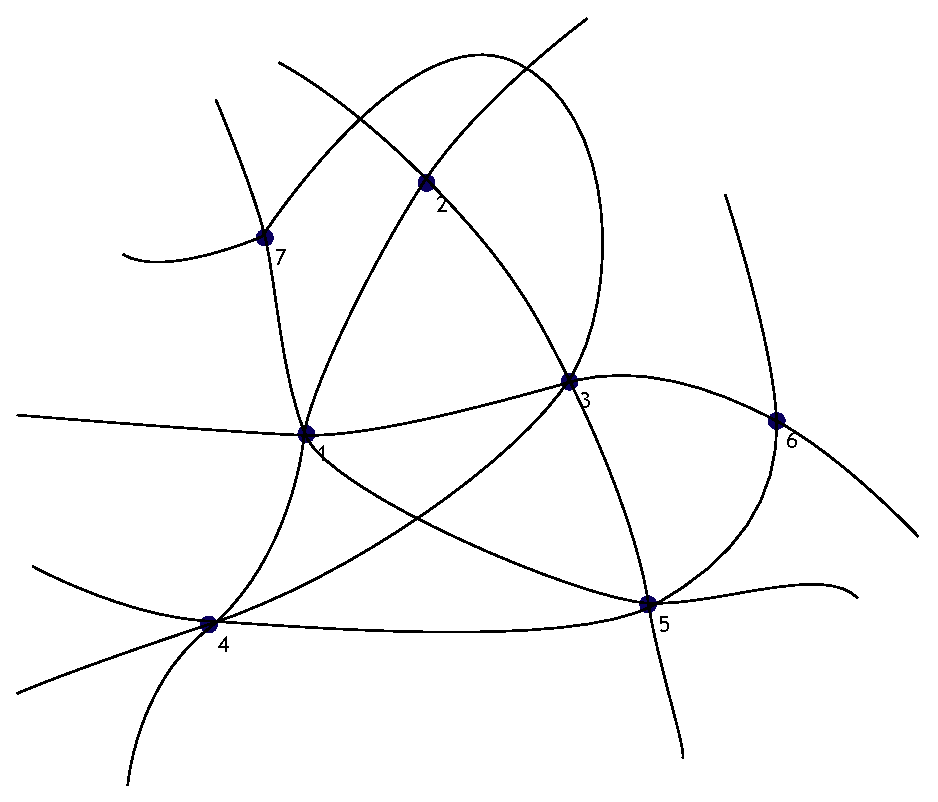
\includegraphics[width=10cm]{finite}\\[20mm]
%	��?.. ���!
\end{center}}


\markboth{Для заметок}{Для заметок}
\newpage\strut
\newpage\strut

\end{document}
